%&preformat-disser
\RequirePackage[l2tabu,orthodox]{nag} % Раскомментировав, можно в логе получать рекомендации относительно правильного использования пакетов и предупреждения об устаревших и нерекомендуемых пакетах
% Формат А4, 14pt (ГОСТ Р 7.0.11-2011, 5.3.6)
\documentclass[a4paper,14pt,oneside,openany]{memoir}

%% Режим черновика
\makeatletter
\@ifundefined{c@draft}{
  \newcounter{draft}
  \setcounter{draft}{1}  		% 0 --- чистовик (максимальное соблюдение ГОСТ)
                         		% 1 --- черновик (отклонения от ГОСТ, но быстрая сборка итоговых PDF)
}{}
\makeatother

%% Использование в pdflatex шрифтов не по-умолчанию
\makeatletter
\@ifundefined{c@usealtfont}{
  \newcounter{usealtfont}
  \setcounter{usealtfont}{1}	% 0 --- шрифты на базе Computer Modern
                               	% 1 --- использовать пакет pscyr, при его наличии
                               	% 2 --- использовать пакет XCharter, при наличии подходящей версии
}{}
\makeatother

%%% Использование в xelatex и lualatex семейств шрифтов %%%
\makeatletter
\@ifundefined{c@fontfamily}{
  \newcounter{fontfamily}
  \setcounter{fontfamily}{1}  % 0 --- CMU семейство. Используется как fallback;
                              % 1 --- Шрифты от MS (Times New Roman и компания)
                              % 2 --- Семейство Liberation
}{}
\makeatother

%% Библиография

%% Внимание! При использовании bibtex8 необходимо удалить все
%% цитирования из  ../common/characteristic.tex
\makeatletter
\@ifundefined{c@bibliosel}{
  \newcounter{bibliosel}
  \setcounter{bibliosel}{0}		% 0 --- встроенная реализация с загрузкой файла через движок bibtex8; 
  								% 1 --- реализация пакетом biblatex через движок biber
}{}
\makeatother

%%% Предкомпиляция tikz рисунков для ускорения работы %%%
\makeatletter
\@ifundefined{c@imgprecompile}{
  \newcounter{imgprecompile}
  \setcounter{imgprecompile}{0}	% 0 --- без предкомпиляции;
  								% 1 --- пользоваться предварительно скомпилированными pdf вместо генерации заново из tikz
}{}
\makeatother
               		 % общие настройки шаблона
%%% Проверка используемого TeX-движка %%%
\RequirePackage{ifxetex, ifluatex}
\newif\ifxetexorluatex   % определяем новый условный оператор (http://tex.stackexchange.com/a/47579)
\ifxetex
    \xetexorluatextrue
\else
    \ifluatex
        \xetexorluatextrue
    \else
        \xetexorluatexfalse
    \fi
\fi

\newif\ifsynopsis           % Условие, проверяющее, что документ --- автореферат

\RequirePackage{etoolbox}[2015/08/02]               % Для продвинутой проверки разных условий

%%% Поля и разметка страницы %%%
\usepackage{pdflscape}                              % Для включения альбомных страниц
\usepackage{geometry}                               % Для последующего задания полей

%%% Математические пакеты %%%
\usepackage{amsthm,amsmath,amscd}   % Математические дополнения от AMS
\usepackage{amsfonts,amssymb}       % Математические дополнения от AMS
\usepackage{mathtools}              % Добавляет окружение multlined

%%%% Установки для размера шрифта 14 pt %%%%
%% Формирование переменных и констант для сравнения (один раз для всех подключаемых файлов)%%
%% должно располагаться до вызова пакета fontspec или polyglossia, потому что они сбивают его работу
\newlength{\curtextsize}
\newlength{\bigtextsize}
\setlength{\bigtextsize}{13.9pt}

\makeatletter
%\show\f@size                                       % неплохо для отслеживания, но вызывает стопорение процесса, если документ компилируется без команды  -interaction=nonstopmode 
\setlength{\curtextsize}{\f@size pt}
\makeatother

%%% Кодировки и шрифты %%%
\ifxetexorluatex
    \usepackage{polyglossia}[2014/05/21]            % Поддержка многоязычности (fontspec подгружается автоматически)
\else
   %%% Решение проблемы копирования текста в буфер кракозябрами
    \ifnumequal{\value{usealtfont}}{0}{}{
        \input glyphtounicode.tex
        \input glyphtounicode-cmr.tex %from pdfx package
        \pdfgentounicode=1
    }
    \usepackage{cmap}                               % Улучшенный поиск русских слов в полученном pdf-файле
    \ifnumequal{\value{usealtfont}}{2}{}{
        \defaulthyphenchar=127                      % Если стоит до fontenc, то переносы не впишутся в выделяемый текст при копировании его в буфер обмена
    }
    \usepackage{textcomp}
    \usepackage[T1,T2A]{fontenc}                    % Поддержка русских букв
    \ifnumequal{\value{usealtfont}}{1}{% Используется pscyr, при наличии
        \IfFileExists{pscyr.sty}{\usepackage{pscyr}}{}  % Подключение pscyr
    }{}
    \usepackage[utf8]{inputenc}[2014/04/30]         % Кодировка utf8
    \usepackage[english, russian]{babel}[2014/03/24]% Языки: русский, английский
    \ifnumequal{\value{usealtfont}}{2}{
        % http://dxdy.ru/post1238763.html#p1238763
        \usepackage[scaled=0.960]{XCharter}[2017/12/19] % Подключение русифицированных шрифтов XCharter
        \usepackage[charter, vvarbb, scaled=1.048]{newtxmath}[2017/12/14]
        \setDisplayskipStretch{-0.078}
    }{}
\fi

%%% Оформление абзацев %%%
\usepackage{indentfirst}                            % Красная строка

%%% Цвета %%%
\usepackage[dvipsnames, table, hyperref, cmyk]{xcolor} % Совместимо с tikz. Конвертация всех цветов в cmyk заложена как удовлетворение возможного требования типографий. Возможно конвертирование и в rgb.

%%% Таблицы %%%
\usepackage{longtable,ltcaption}                    % Длинные таблицы
\usepackage{multirow,makecell}                      % Улучшенное форматирование таблиц

%%% Общее форматирование
\usepackage{soulutf8}                               % Поддержка переносоустойчивых подчёркиваний и зачёркиваний
\usepackage{icomma}                                 % Запятая в десятичных дробях

%%% Оптимизация расстановки переносов и длины последней строки абзаца
\ifluatex
    \ifnumequal{\value{draft}}{1}{% Черновик
        \usepackage[hyphenation, lastparline, nosingleletter, homeoarchy,
        rivers, draft]{impnattypo}
    }{% Чистовик
        \usepackage[hyphenation, lastparline, nosingleletter]{impnattypo}
    }
\else
    \usepackage[hyphenation, lastparline]{impnattypo}
\fi

%%% Гиперссылки %%%
\usepackage{hyperref}[2012/11/06]

%%% Изображения %%%
\usepackage{graphicx}[2014/04/25]                   % Подключаем пакет работы с графикой

%%% Списки %%%
\usepackage{enumitem}

%%% Счётчики %%%
\usepackage[figure,table]{totalcount}               % Счётчик рисунков и таблиц
\usepackage{totcount}                               % Пакет создания счётчиков на основе последнего номера подсчитываемого элемента (может требовать дважды компилировать документ)
\usepackage{totpages}                               % Счётчик страниц, совместимый с hyperref (ссылается на номер последней страницы). Желательно ставить последним пакетом в преамбуле

%%% Продвинутое управление групповыми ссылками (пока только формулами) %%%
\ifxetexorluatex
    \usepackage{cleveref}                           % cleveref корректно считывает язык из настроек polyglossia
\else
    \usepackage[russian]{cleveref}                  % cleveref имеет сложности со считыванием языка из babel. Такое решение русификации вывода выбрано вместо определения в documentclass из опасности что-то лишнее передать во все остальные пакеты, включая библиографию.
\fi
\creflabelformat{equation}{#2#1#3}                  % Формат по умолчанию ставил круглые скобки вокруг каждого номера ссылки, теперь просто номера ссылок без какого-либо дополнительного оформления
\crefrangelabelformat{equation}{#3#1#4\cyrdash#5#2#6}   % Интервалы в русском языке принято делать через тире, если иное не оговорено


\ifnumequal{\value{draft}}{1}{% Черновик
    \usepackage[firstpage]{draftwatermark}
    \SetWatermarkText{DRAFT}
    \SetWatermarkFontSize{14pt}
    \SetWatermarkScale{15}
    \SetWatermarkAngle{45}
}{}

%%% Цитата, не приводимая в автореферате:
% возможно, актуальна только для biblatex
%\newcommand{\citeinsynopsis}[1]{\ifsynopsis\else ~\cite{#1} \fi}
  				 % Пакеты общие для диссертации и автореферата
\synopsisfalse                           % Этот документ --- не автореферат
%%% Прикладные пакеты %%% 
%\usepackage{calc}               % Пакет для расчётов параметров, например длины

%%% Для добавления Стр. над номерами страниц в оглавлении
%%% http://tex.stackexchange.com/a/306950
\usepackage{afterpage}

\usepackage{tikz}                   % Продвинутый пакет векторной графики
\usetikzlibrary{chains}             % Для примера tikz рисунка
\usetikzlibrary{shapes.geometric}   % Для примера tikz рисунка
\usetikzlibrary{shapes.symbols}     % Для примера tikz рисунка
\usetikzlibrary{arrows}             % Для примера tikz рисунка
\ifnumequal{\value{imgprecompile}}{1}{% Только если у нас включена предкомпиляция
    \usetikzlibrary{external}   % подключение возможности предкомпиляции
    \tikzexternalize[prefix=Dissertation/images/] % activate! % здесь можно указать отдельную папку для скомпилированных файлов
    \ifxetex
        \tikzset{external/up to date check={diff}}
    \fi
}{}
         % Пакеты для диссертации
\usepackage{tabu, tabulary}  %таблицы с автоматически подбирающейся шириной столбцов
\usepackage{fr-longtable}    %ради \endlasthead

% Листинги с исходным кодом программ
\usepackage{fancyvrb}
\usepackage{listings}
\lccode`\~=0\relax %Без этого хака из-за особенностей пакета listings перестают работать конструкции с \MakeLowercase и т. п. в (xe|lua)latex

% Русская традиция начертания греческих букв
\usepackage{upgreek} % прямые греческие ради русской традиции

%%% Микротипографика
%\ifnumequal{\value{draft}}{0}{% Только если у нас режим чистовика
%    \usepackage[final, babel, shrink=45]{microtype}[2016/05/14] % улучшает представление букв и слов в строках, может помочь при наличии отдельно висящих слов
%}{}

% Отметка о версии черновика на каждой странице
% Чтобы работало надо в своей локальной копии по инструкции
% https://www.ctan.org/pkg/gitinfo2 создать небходимые файлы в папке
% ./git/hooks
% If you’re familiar with tweaking git, you can probably work it out for
% yourself. If not, I suggest you follow these steps:
% 1. First, you need a git repository and working tree. For this example,
% let’s suppose that the root of the working tree is in ~/compsci
% 2. Copy the file post-xxx-sample.txt (which is in the same folder of
% your TEX distribution as this pdf) into the git hooks directory in your
% working copy. In our example case, you should end up with a file called
% ~/compsci/.git/hooks/post-checkout
% 3. If you’re using a unix-like system, don’t forget to make the file executable.
% Just how you do this is outside the scope of this manual, but one
% possible way is with commands such as this:
% chmod g+x post-checkout.
% 4. Test your setup with “git checkout master” (or another suitable branch
% name). This should generate copies of gitHeadInfo.gin in the directories
% you intended.
% 5. Now make two more copies of this file in the same directory (hooks),
% calling them post-commit and post-merge, and you’re done. As before,
% users of unix-like systems should ensure these files are marked as
% executable.
\ifnumequal{\value{draft}}{1}{% Черновик
   \IfFileExists{.git/gitHeadInfo.gin}{                                        
      \usepackage[mark,pcount]{gitinfo2}
      \renewcommand{\gitMark}{rev.\gitAbbrevHash\quad\gitCommitterEmail\quad\gitAuthorIsoDate}
      \renewcommand{\gitMarkFormat}{\rmfamily\color{Gray}\small\bfseries}
   }{}
}{}        % Пакеты для специфических пользовательских задач

%% Режим черновика
\makeatletter
\@ifundefined{c@draft}{
  \newcounter{draft}
  \setcounter{draft}{1}  		% 0 --- чистовик (максимальное соблюдение ГОСТ)
                         		% 1 --- черновик (отклонения от ГОСТ, но быстрая сборка итоговых PDF)
}{}
\makeatother

%% Использование в pdflatex шрифтов не по-умолчанию
\makeatletter
\@ifundefined{c@usealtfont}{
  \newcounter{usealtfont}
  \setcounter{usealtfont}{1}	% 0 --- шрифты на базе Computer Modern
                               	% 1 --- использовать пакет pscyr, при его наличии
                               	% 2 --- использовать пакет XCharter, при наличии подходящей версии
}{}
\makeatother

%%% Использование в xelatex и lualatex семейств шрифтов %%%
\makeatletter
\@ifundefined{c@fontfamily}{
  \newcounter{fontfamily}
  \setcounter{fontfamily}{1}  % 0 --- CMU семейство. Используется как fallback;
                              % 1 --- Шрифты от MS (Times New Roman и компания)
                              % 2 --- Семейство Liberation
}{}
\makeatother

%% Библиография

%% Внимание! При использовании bibtex8 необходимо удалить все
%% цитирования из  ../common/characteristic.tex
\makeatletter
\@ifundefined{c@bibliosel}{
  \newcounter{bibliosel}
  \setcounter{bibliosel}{0}		% 0 --- встроенная реализация с загрузкой файла через движок bibtex8; 
  								% 1 --- реализация пакетом biblatex через движок biber
}{}
\makeatother

%%% Предкомпиляция tikz рисунков для ускорения работы %%%
\makeatletter
\@ifundefined{c@imgprecompile}{
  \newcounter{imgprecompile}
  \setcounter{imgprecompile}{0}	% 0 --- без предкомпиляции;
  								% 1 --- пользоваться предварительно скомпилированными pdf вместо генерации заново из tikz
}{}
\makeatother
      % Упрощённые настройки шаблона

\input{Dissertation/preamblenames}       % Переопределение именований, чтобы можно было и в преамбуле использовать
\input{common/newnames}  				 % Новые переменные, которые могут использоваться во всём проекте

%%% Основные сведения %%%
\newcommand{\thesisAuthorLastName}{\todo{Рахматова}}
\newcommand{\thesisAuthorOtherNames}{\todo{Нателла Ильтефат-гызы}}
\newcommand{\thesisAuthorInitials}{\todo{Н.\,И.}}
\newcommand{\thesisAuthor}             % Диссертация, ФИО автора
{%
    \texorpdfstring{% \texorpdfstring takes two arguments and uses the first for (La)TeX and the second for pdf
        \thesisAuthorLastName~\thesisAuthorOtherNames% так будет отображаться на титульном листе или в тексте, где будет использоваться переменная
    }{%
        \thesisAuthorLastName, \thesisAuthorOtherNames% эта запись для свойств pdf-файла. В таком виде, если pdf будет обработан программами для сбора библиографических сведений, будет правильно представлена фамилия.
    }
}
\newcommand{\thesisAuthorShort}        % Диссертация, ФИО автора инициалами
{\thesisAuthorInitials~\thesisAuthorLastName}
%\newcommand{\thesisUdk}                % Диссертация, УДК
%{\todo{xxx.xxx}}
\newcommand{\thesisTitle}              % Диссертация, название
{\todo{Засуха и все, все, все}}
\newcommand{\thesisSpecialtyNumber}    % Диссертация, специальность, номер
{\todo{XX.XX.XX}}
\newcommand{\thesisSpecialtyTitle}     % Диссертация, специальность, название
{\todo{Название специальности}}
\newcommand{\thesisDegree}             % Диссертация, ученая степень
{\todo{кандидата географических наук}}
\newcommand{\thesisDegreeShort}        % Диссертация, ученая степень, краткая запись
{\todo{канд. геогр. наук}}
\newcommand{\thesisCity}               % Диссертация, город написания диссертации
{\todo{Ташкент}}
\newcommand{\thesisYear}               % Диссертация, год написания диссертации
{\todo{2018}}
\newcommand{\thesisOrganization}       % Диссертация, организация
{\todo{Институт}}
\newcommand{\thesisOrganizationShort}  % Диссертация, краткое название организации для доклада
{\todo{НазУчДисРаб}}

\newcommand{\thesisInOrganization}     % Диссертация, организация в предложном падеже: Работа выполнена в ...
{\todo{учреждении, в~котором выполнялась данная диссертационная работа}}

\newcommand{\supervisorFio}            % Научный руководитель, ФИО
{\todo{Фамилия Имя Отчество}}
\newcommand{\supervisorRegalia}        % Научный руководитель, регалии
{\todo{уч. степень, уч. звание}}
\newcommand{\supervisorFioShort}       % Научный руководитель, ФИО
{\todo{И.\,О.~Фамилия}}
\newcommand{\supervisorRegaliaShort}   % Научный руководитель, регалии
{\todo{уч.~ст.,~уч.~зв.}}


\newcommand{\opponentOneFio}           % Оппонент 1, ФИО
{\todo{Фамилия Имя Отчество}}
\newcommand{\opponentOneRegalia}       % Оппонент 1, регалии
{\todo{доктор физико-математических наук, профессор}}
\newcommand{\opponentOneJobPlace}      % Оппонент 1, место работы
{\todo{Не очень длинное название для места работы}}
\newcommand{\opponentOneJobPost}       % Оппонент 1, должность
{\todo{старший научный сотрудник}}

\newcommand{\opponentTwoFio}           % Оппонент 2, ФИО
{\todo{Фамилия Имя Отчество}}
\newcommand{\opponentTwoRegalia}       % Оппонент 2, регалии
{\todo{кандидат физико-математических наук}}
\newcommand{\opponentTwoJobPlace}      % Оппонент 2, место работы
{\todo{Основное место работы c длинным длинным длинным длинным названием}}
\newcommand{\opponentTwoJobPost}       % Оппонент 2, должность
{\todo{старший научный сотрудник}}

\newcommand{\leadingOrganizationTitle} % Ведущая организация, дополнительные строки
{\todo{Федеральное государственное бюджетное образовательное учреждение высшего профессионального образования с~длинным длинным длинным длинным названием}}

\newcommand{\defenseDate}              % Защита, дата
{\todo{DD mmmmmmmm YYYY~г.~в~XX часов}}
\newcommand{\defenseCouncilNumber}     % Защита, номер диссертационного совета
{\todo{Д\,123.456.78}}
\newcommand{\defenseCouncilTitle}      % Защита, учреждение диссертационного совета
{\todo{Название учреждения}}
\newcommand{\defenseCouncilAddress}    % Защита, адрес учреждение диссертационного совета
{\todo{Адрес}}
\newcommand{\defenseCouncilPhone}      % Телефон для справок
{\todo{+7~(0000)~00-00-00}}

\newcommand{\defenseSecretaryFio}      % Секретарь диссертационного совета, ФИО
{\todo{Фамилия Имя Отчество}}
\newcommand{\defenseSecretaryRegalia}  % Секретарь диссертационного совета, регалии
{\todo{д-р~физ.-мат. наук}}            % Для сокращений есть ГОСТы, например: ГОСТ Р 7.0.12-2011 + http://base.garant.ru/179724/#block_30000

\newcommand{\synopsisLibrary}          % Автореферат, название библиотеки
{\todo{Название библиотеки}}
\newcommand{\synopsisDate}             % Автореферат, дата рассылки
{\todo{DD mmmmmmmm YYYY года}}

% To avoid conflict with beamer class use \providecommand
\providecommand{\keywords}%            % Ключевые слова для метаданных PDF диссертации и автореферата
{}
      				 % Основные сведения
%%% Шаблон %%%
\DeclareRobustCommand{\todo}{\textcolor{red}}       % решаем проблему превращения названия цвета в результате \MakeUppercase, http://tex.stackexchange.com/a/187930, \DeclareRobustCommand protects \todo from expanding inside \MakeUppercase
\AtBeginDocument{%
    \setlength{\parindent}{2.5em}                   % Абзацный отступ. Должен быть одинаковым по всему тексту и равен пяти знакам (ГОСТ Р 7.0.11-2011, 5.3.7).
}

%%% Подписи %%%
\setlength{\abovecaptionskip}{0pt}   % Отбивка над подписью
\setlength{\belowcaptionskip}{0pt}   % Отбивка под подписью
\captionwidth{\linewidth}
\normalcaptionwidth

%%% Таблицы %%%
\ifnumequal{\value{tabcap}}{0}{%
    \newcommand{\tabcapalign}{\raggedright}  % по левому краю страницы или аналога parbox
    \renewcommand{\tablabelsep}{~\cyrdash\ } % тире как разделитель идентификатора с номером от наименования
    \newcommand{\tabtitalign}{}
}{%
    \ifnumequal{\value{tablaba}}{0}{%
        \newcommand{\tabcapalign}{\raggedright}  % по левому краю страницы или аналога parbox
    }{}

    \ifnumequal{\value{tablaba}}{1}{%
        \newcommand{\tabcapalign}{\centering}    % по центру страницы или аналога parbox
    }{}

    \ifnumequal{\value{tablaba}}{2}{%
        \newcommand{\tabcapalign}{\raggedleft}   % по правому краю страницы или аналога parbox
    }{}

    \ifnumequal{\value{tabtita}}{0}{%
        \newcommand{\tabtitalign}{\par\raggedright}  % по левому краю страницы или аналога parbox
    }{}

    \ifnumequal{\value{tabtita}}{1}{%
        \newcommand{\tabtitalign}{\par\centering}    % по центру страницы или аналога parbox
    }{}

    \ifnumequal{\value{tabtita}}{2}{%
        \newcommand{\tabtitalign}{\par\raggedleft}   % по правому краю страницы или аналога parbox
    }{}
}

\precaption{\tabcapalign} % всегда идет перед подписью или \legend
\captionnamefont{\normalfont\normalsize} % Шрифт надписи «Таблица #»; также определяет шрифт у \legend
\captiondelim{\tablabelsep} % разделитель идентификатора с номером от наименования
\captionstyle[\tabtitalign]{\tabtitalign}
\captiontitlefont{\normalfont\normalsize} % Шрифт с текстом подписи

%%% Рисунки %%%
\setfloatadjustment{figure}{%
    \setlength{\abovecaptionskip}{0pt}   % Отбивка над подписью
    \setlength{\belowcaptionskip}{0pt}   % Отбивка под подписью
    \precaption{} % всегда идет перед подписью или \legend
    \captionnamefont{\normalfont\normalsize} % Шрифт надписи «Рисунок #»; также определяет шрифт у \legend
    \captiondelim{\figlabelsep} % разделитель идентификатора с номером от наименования
    \captionstyle[\centering]{\centering} % Центрирование подписей, заданных командой \caption и \legend
    \captiontitlefont{\normalfont\normalsize} % Шрифт с текстом подписи
    \postcaption{} % всегда идет после подписи или \legend, и с новой строки
}

%%% Подписи подрисунков %%%
\newsubfloat{figure} % Включает возможность использовать подрисунки у окружений figure
\renewcommand{\thesubfigure}{\asbuk{subfigure}}           % Буквенные номера подрисунков
\subcaptionsize{\normalsize} % Шрифт подписи названий подрисунков (не отличается от основного)
\subcaptionlabelfont{\normalfont}
\subcaptionfont{\!\!) \normalfont} % Вот так тут добавили скобку после буквы.
\subcaptionstyle{\centering}
%\subcaptionsize{\fontsize{12pt}{13pt}\selectfont} % объявляем шрифт 12pt для использования в подписях, тут же надо интерлиньяж объявлять, если не наследуется

%%% Настройки гиперссылок %%%
\ifluatex
    \hypersetup{
        unicode,                % Unicode encoded PDF strings
    }
\fi

\hypersetup{
    linktocpage=true,           % ссылки с номера страницы в оглавлении, списке таблиц и списке рисунков
%    linktoc=all,                % both the section and page part are links
%    pdfpagelabels=false,        % set PDF page labels (true|false)
    plainpages=false,           % Forces page anchors to be named by the Arabic form  of the page number, rather than the formatted form
    colorlinks,                 % ссылки отображаются раскрашенным текстом, а не раскрашенным прямоугольником, вокруг текста
    linkcolor={linkcolor},      % цвет ссылок типа ref, eqref и подобных
    citecolor={citecolor},      % цвет ссылок-цитат
    urlcolor={urlcolor},        % цвет гиперссылок
%    hidelinks,                  % Hide links (removing color and border)
    pdftitle={\thesisTitle},    % Заголовок
    pdfauthor={\thesisAuthor},  % Автор
    pdfsubject={\thesisSpecialtyNumber\ \thesisSpecialtyTitle},      % Тема
%    pdfcreator={Создатель},     % Создатель, Приложение
%    pdfproducer={Производитель},% Производитель, Производитель PDF
    pdfkeywords={\keywords},    % Ключевые слова
    pdflang={ru},
}
\ifnumequal{\value{draft}}{1}{% Черновик
    \hypersetup{
        draft,
    }
}{}

%%% Списки %%%
% Используем короткое тире (endash) для ненумерованных списков (ГОСТ 2.105-95, пункт 4.1.7, требует дефиса, но так лучше смотрится)
\renewcommand{\labelitemi}{\normalfont\bfseries{--}}

% Перечисление строчными буквами латинского алфавита (ГОСТ 2.105-95, 4.1.7)
%\renewcommand{\theenumi}{\alph{enumi}}
%\renewcommand{\labelenumi}{\theenumi)} 

% Перечисление строчными буквами русского алфавита (ГОСТ 2.105-95, 4.1.7)
\makeatletter
\AddEnumerateCounter{\asbuk}{\russian@alph}{щ}      % Управляем списками/перечислениями через пакет enumitem, а он 'не знает' про asbuk, потому 'учим' его
\makeatother
%\renewcommand{\theenumi}{\asbuk{enumi}} %первый уровень нумерации
%\renewcommand{\labelenumi}{\theenumi)} %первый уровень нумерации 
\renewcommand{\theenumii}{\asbuk{enumii}} %второй уровень нумерации
\renewcommand{\labelenumii}{\theenumii)} %второй уровень нумерации 
\renewcommand{\theenumiii}{\arabic{enumiii}} %третий уровень нумерации
\renewcommand{\labelenumiii}{\theenumiii)} %третий уровень нумерации 

\setlist{nosep,%                                    % Единый стиль для всех списков (пакет enumitem), без дополнительных интервалов.
    labelindent=\parindent,leftmargin=*%            % Каждый пункт, подпункт и перечисление записывают с абзацного отступа (ГОСТ 2.105-95, 4.1.8)
}
    				 % Стили общие для диссертации и автореферата
%%% Переопределение именований, если иначе не сработает %%%
%\gappto\captionsrussian{
%    \renewcommand{\chaptername}{Глава}
%    \renewcommand{\appendixname}{Приложение} % (ГОСТ Р 7.0.11-2011, 5.7)
%}

%%% Изображения %%%
\graphicspath{{images/}{Dissertation/images/}}         % Пути к изображениям

%%% Интервалы %%%
%% По ГОСТ Р 7.0.11-2011, пункту 5.3.6 требуется полуторный интервал
%% Реализация средствами класса (на основе setspace) ближе к типографской классике.
%% И правит сразу и в таблицах (если со звёздочкой)
%\DoubleSpacing*     % Двойной интервал
\OnehalfSpacing*    % Полуторный интервал
%\setSpacing{1.42}   % Полуторный интервал, подобный Ворду (возможно, стоит включать вместе с предыдущей строкой)

%%% Макет страницы %%%
% Выставляем значения полей (ГОСТ 7.0.11-2011, 5.3.7)
\geometry{a4paper, top=2cm, bottom=2cm, left=2.5cm, right=1cm, nofoot, nomarginpar} %, heightrounded, showframe
\setlength{\topskip}{0pt}   %размер дополнительного верхнего поля
\setlength{\footskip}{12.3pt} % снимет warning, согласно https://tex.stackexchange.com/a/334346

%%% Выравнивание и переносы %%%
%% http://tex.stackexchange.com/questions/241343/what-is-the-meaning-of-fussy-sloppy-emergencystretch-tolerance-hbadness
%% http://www.latex-community.org/forum/viewtopic.php?p=70342#p70342
\tolerance 1414
\hbadness 1414
\emergencystretch 1.5em % В случае проблем регулировать в первую очередь
\hfuzz 0.3pt
\vfuzz \hfuzz
%\raggedbottom
%\sloppy                 % Избавляемся от переполнений
\clubpenalty=10000      % Запрещаем разрыв страницы после первой строки абзаца
\widowpenalty=10000     % Запрещаем разрыв страницы после последней строки абзаца
\brokenpenalty=4991     % Ограничение на разрыв страницы, если строка заканчивается переносом

%%% Блок управления параметрами для выравнивания заголовков в тексте %%%
\newlength{\otstuplen}
\setlength{\otstuplen}{\theotstup\parindent}
\ifnumequal{\value{headingalign}}{0}{% выравнивание заголовков в тексте
    \newcommand{\hdngalign}{\centering}                % по центру
    \newcommand{\hdngaligni}{}% по центру
    \setlength{\otstuplen}{0pt}
}{%
    \newcommand{\hdngalign}{}                 % по левому краю
    \newcommand{\hdngaligni}{\hspace{\otstuplen}}      % по левому краю
} % В обоих случаях вроде бы без переноса, как и надо (ГОСТ Р 7.0.11-2011, 5.3.5)

%%% Оглавление %%%
\renewcommand{\cftchapterdotsep}{\cftdotsep}                % отбивка точками до номера страницы начала главы/раздела

%% Переносить слова в заголовке не допускается (ГОСТ Р 7.0.11-2011, 5.3.5). Заголовки в оглавлении должны точно повторять заголовки в тексте (ГОСТ Р 7.0.11-2011, 5.2.3). Прямого указания на запрет переносов в оглавлении нет, но по той же логике невнесения искажений в смысл, лучше в оглавлении не переносить:
\setrmarg{2.55em plus1fil}                             %To have the (sectional) titles in the ToC, etc., typeset ragged right with no hyphenation
\renewcommand{\cftchapterpagefont}{\normalfont}        % нежирные номера страниц у глав в оглавлении
\renewcommand{\cftchapterleader}{\cftdotfill{\cftchapterdotsep}}% нежирные точки до номеров страниц у глав в оглавлении
%\renewcommand{\cftchapterfont}{}                       % нежирные названия глав в оглавлении

\ifnumgreater{\value{headingdelim}}{0}{%
    \renewcommand\cftchapteraftersnum{.\space}       % добавляет точку с пробелом после номера раздела в оглавлении
}{}
\ifnumgreater{\value{headingdelim}}{1}{%
    \renewcommand\cftsectionaftersnum{.\space}       % добавляет точку с пробелом после номера подраздела в оглавлении
    \renewcommand\cftsubsectionaftersnum{.\space}    % добавляет точку с пробелом после номера подподраздела в оглавлении
    \renewcommand\cftsubsubsectionaftersnum{.\space} % добавляет точку с пробелом после номера подподподраздела в оглавлении
    \AtBeginDocument{% без этого polyglossia сама всё переопределяет
        \setsecnumformat{\csname the#1\endcsname.\space}
    }
}{%
    \AtBeginDocument{% без этого polyglossia сама всё переопределяет
        \setsecnumformat{\csname the#1\endcsname\quad}
    }
}

\renewcommand*{\cftappendixname}{\appendixname\space} % Слово Приложение в оглавлении

%%% Колонтитулы %%%
% Порядковый номер страницы печатают на середине верхнего поля страницы (ГОСТ Р 7.0.11-2011, 5.3.8)
\makeevenhead{plain}{}{\thepage}{}
\makeoddhead{plain}{}{\thepage}{}
\makeevenfoot{plain}{}{}{}
\makeoddfoot{plain}{}{}{}
\pagestyle{plain}

%%% добавить Стр. над номерами страниц в оглавлении
%%% http://tex.stackexchange.com/a/306950
\newif\ifendTOC

\newcommand*{\tocheader}{
\ifnumequal{\value{pgnum}}{1}{%
    \ifendTOC\else\hbox to \linewidth%
      {\noindent{}~\hfill{Стр.}}\par%
      \ifnumless{\value{page}}{3}{}{%
        \vspace{0.5\onelineskip}
      }
      \afterpage{\tocheader}
    \fi%
}{}%
}%

%%% Оформление заголовков глав, разделов, подразделов %%%
%% Работа должна быть выполнена ... размером шрифта 12-14 пунктов (ГОСТ Р 7.0.11-2011, 5.3.8). То есть не должно быть надписей шрифтом более 14. Так и поставим.
%% Эти установки будут давать одинаковый результат независимо от выбора базовым шрифтом 12 пт или 14 пт
\newcommand{\basegostsectionfont}{\fontsize{14pt}{16pt}\selectfont\bfseries}

\makechapterstyle{thesisgost}{%
    \chapterstyle{default}
    \setlength{\beforechapskip}{0pt}
    \setlength{\midchapskip}{0pt}
    \setlength{\afterchapskip}{\theintvl\curtextsize}
    \renewcommand*{\chapnamefont}{\basegostsectionfont}
    \renewcommand*{\chapnumfont}{\basegostsectionfont}
    \renewcommand*{\chaptitlefont}{\basegostsectionfont}
    \renewcommand*{\chapterheadstart}{}
    \ifnumgreater{\value{headingdelim}}{0}{%
        \renewcommand*{\afterchapternum}{.\space}   % добавляет точку с пробелом после номера раздела
    }{%
        \renewcommand*{\afterchapternum}{\quad}     % добавляет \quad после номера раздела
    }
    \renewcommand*{\printchapternum}{\hdngaligni\hdngalign\chapnumfont \thechapter}
    \renewcommand*{\printchaptername}{}
    \renewcommand*{\printchapternonum}{\hdngaligni\hdngalign}
}

\makeatletter
\makechapterstyle{thesisgostchapname}{%
    \chapterstyle{thesisgost}
    \renewcommand*{\printchapternum}{\chapnumfont \thechapter}
    \renewcommand*{\printchaptername}{\hdngaligni\hdngalign\chapnamefont \@chapapp} %
}
\makeatother

\chapterstyle{thesisgost}

\setsecheadstyle{\basegostsectionfont\hdngalign}
\setsecindent{\otstuplen}

\setsubsecheadstyle{\basegostsectionfont\hdngalign}
\setsubsecindent{\otstuplen}

\setsubsubsecheadstyle{\basegostsectionfont\hdngalign}
\setsubsubsecindent{\otstuplen}

\sethangfrom{\noindent #1} %все заголовки подразделов центрируются с учетом номера, как block

\ifnumequal{\value{chapstyle}}{1}{%
    \chapterstyle{thesisgostchapname}
    \renewcommand*{\cftchaptername}{\chaptername\space} % будет вписано слово Глава перед каждым номером раздела в оглавлении
}{}%

%%% Интервалы между заголовками
\setbeforesecskip{\theintvl\curtextsize}% Заголовки отделяют от текста сверху и снизу тремя интервалами (ГОСТ Р 7.0.11-2011, 5.3.5).
\setaftersecskip{\theintvl\curtextsize}
\setbeforesubsecskip{\theintvl\curtextsize}
\setaftersubsecskip{\theintvl\curtextsize}
\setbeforesubsubsecskip{\theintvl\curtextsize}
\setaftersubsubsecskip{\theintvl\curtextsize}

%%% Блок дополнительного управления размерами заголовков
\ifnumequal{\value{headingsize}}{1}{% Пропорциональные заголовки и базовый шрифт 14 пт
    \renewcommand{\basegostsectionfont}{\large\bfseries}
    \renewcommand*{\chapnamefont}{\Large\bfseries}
    \renewcommand*{\chapnumfont}{\Large\bfseries}
    \renewcommand*{\chaptitlefont}{\Large\bfseries}
}{}

%%% Счётчики %%%

%% Упрощённые настройки шаблона диссертации: нумерация формул, таблиц, рисунков
\ifnumequal{\value{contnumeq}}{1}{%
    \counterwithout{equation}{chapter} % Убираем связанность номера формулы с номером главы/раздела
}{}
\ifnumequal{\value{contnumfig}}{1}{%
    \counterwithout{figure}{chapter}   % Убираем связанность номера рисунка с номером главы/раздела
}{}
\ifnumequal{\value{contnumtab}}{1}{%
    \counterwithout{table}{chapter}    % Убираем связанность номера таблицы с номером главы/раздела
}{}


%%http://www.linux.org.ru/forum/general/6993203#comment-6994589 (используется totcount)
\makeatletter
\def\formbytotal#1#2#3#4#5{%
    \newcount\@c
    \@c\totvalue{#1}\relax
    \newcount\@last
    \newcount\@pnul
    \@last\@c\relax
    \divide\@last 10
    \@pnul\@last\relax
    \divide\@pnul 10
    \multiply\@pnul-10
    \advance\@pnul\@last
    \multiply\@last-10
    \advance\@last\@c
    \total{#1}~#2%
    \ifnum\@pnul=1#5\else%
    \ifcase\@last#5\or#3\or#4\or#4\or#4\else#5\fi
    \fi
}
\makeatother

\AtBeginDocument{
%% регистрируем счётчики в системе totcounter
    \regtotcounter{totalcount@figure}
    \regtotcounter{totalcount@table}       % Если иным способом поставить в преамбуле то ошибка в числе таблиц
    \regtotcounter{TotPages}               % Если иным способом поставить в преамбуле то ошибка в числе страниц
}

%%% Правильная нумерация приложений %%%
%% По ГОСТ 2.105, п. 4.3.8 Приложения обозначают заглавными буквами русского алфавита,
%% начиная с А, за исключением букв Ё, З, Й, О, Ч, Ь, Ы, Ъ.
%% Здесь также переделаны все нумерации русскими буквами.
\ifxetexorluatex
    \makeatletter
    \def\russian@Alph#1{\ifcase#1\or
       А\or Б\or В\or Г\or Д\or Е\or Ж\or
       И\or К\or Л\or М\or Н\or
       П\or Р\or С\or Т\or У\or Ф\or Х\or
       Ц\or Ш\or Щ\or Э\or Ю\or Я\else\xpg@ill@value{#1}{russian@Alph}\fi}
    \def\russian@alph#1{\ifcase#1\or
       а\or б\or в\or г\or д\or е\or ж\or
       и\or к\or л\or м\or н\or
       п\or р\or с\or т\or у\or ф\or х\or
       ц\or ш\or щ\or э\or ю\or я\else\xpg@ill@value{#1}{russian@alph}\fi}
    \makeatother
\else
    \makeatletter
    \if@uni@ode
      \def\russian@Alph#1{\ifcase#1\or
        А\or Б\or В\or Г\or Д\or Е\or Ж\or
        И\or К\or Л\or М\or Н\or
        П\or Р\or С\or Т\or У\or Ф\or Х\or
        Ц\or Ш\or Щ\or Э\or Ю\or Я\else\@ctrerr\fi}
    \else
      \def\russian@Alph#1{\ifcase#1\or
        \CYRA\or\CYRB\or\CYRV\or\CYRG\or\CYRD\or\CYRE\or\CYRZH\or
        \CYRI\or\CYRK\or\CYRL\or\CYRM\or\CYRN\or
        \CYRP\or\CYRR\or\CYRS\or\CYRT\or\CYRU\or\CYRF\or\CYRH\or
        \CYRC\or\CYRSH\or\CYRSHCH\or\CYREREV\or\CYRYU\or
        \CYRYA\else\@ctrerr\fi}
    \fi
    \if@uni@ode
      \def\russian@alph#1{\ifcase#1\or
        а\or б\or в\or г\or д\or е\or ж\or
        и\or к\or л\or м\or н\or
        п\or р\or с\or т\or у\or ф\or х\or
        ц\or ш\or щ\or э\or ю\or я\else\@ctrerr\fi}
    \else
      \def\russian@alph#1{\ifcase#1\or
        \cyra\or\cyrb\or\cyrv\or\cyrg\or\cyrd\or\cyre\or\cyrzh\or
        \cyri\or\cyrk\or\cyrl\or\cyrm\or\cyrn\or
        \cyrp\or\cyrr\or\cyrs\or\cyrt\or\cyru\or\cyrf\or\cyrh\or
        \cyrc\or\cyrsh\or\cyrshch\or\cyrerev\or\cyryu\or
        \cyrya\else\@ctrerr\fi}
    \fi
    \makeatother
\fi
           % Стили для диссертации
% для вертикального центрирования ячеек в tabulary
\def\zz{\ifx\[$\else\aftergroup\zzz\fi}
%$ \] % <-- чиним подсветку синтаксиса в некоторых редакторах
\def\zzz{\setbox0\lastbox
\dimen0\dimexpr\extrarowheight + \ht0-\dp0\relax
\setbox0\hbox{\raise-.5\dimen0\box0}%
\ht0=\dimexpr\ht0+\extrarowheight\relax
\dp0=\dimexpr\dp0+\extrarowheight\relax 
\box0
}



\lstdefinelanguage{Renhanced}%
{keywords={abbreviate,abline,abs,acos,acosh,action,add1,add,%
        aggregate,alias,Alias,alist,all,anova,any,aov,aperm,append,apply,%
        approx,approxfun,apropos,Arg,args,array,arrows,as,asin,asinh,%
        atan,atan2,atanh,attach,attr,attributes,autoload,autoloader,ave,%
        axis,backsolve,barplot,basename,besselI,besselJ,besselK,besselY,%
        beta,binomial,body,box,boxplot,break,browser,bug,builtins,bxp,by,%
        c,C,call,Call,case,cat,category,cbind,ceiling,character,char,%
        charmatch,check,chol,chol2inv,choose,chull,class,close,cm,codes,%
        coef,coefficients,co,col,colnames,colors,colours,commandArgs,%
        comment,complete,complex,conflicts,Conj,contents,contour,%
        contrasts,contr,control,helmert,contrib,convolve,cooks,coords,%
        distance,coplot,cor,cos,cosh,count,fields,cov,covratio,wt,CRAN,%
        create,crossprod,cummax,cummin,cumprod,cumsum,curve,cut,cycle,D,%
        data,dataentry,date,dbeta,dbinom,dcauchy,dchisq,de,debug,%
        debugger,Defunct,default,delay,delete,deltat,demo,de,density,%
        deparse,dependencies,Deprecated,deriv,description,detach,%
        dev2bitmap,dev,cur,deviance,off,prev,,dexp,df,dfbetas,dffits,%
        dgamma,dgeom,dget,dhyper,diag,diff,digamma,dim,dimnames,dir,%
        dirname,dlnorm,dlogis,dnbinom,dnchisq,dnorm,do,dotplot,double,%
        download,dpois,dput,drop,drop1,dsignrank,dt,dummy,dump,dunif,%
        duplicated,dweibull,dwilcox,dyn,edit,eff,effects,eigen,else,%
        emacs,end,environment,env,erase,eval,equal,evalq,example,exists,%
        exit,exp,expand,expression,External,extract,extractAIC,factor,%
        fail,family,fft,file,filled,find,fitted,fivenum,fix,floor,for,%
        For,formals,format,formatC,formula,Fortran,forwardsolve,frame,%
        frequency,ftable,ftable2table,function,gamma,Gamma,gammaCody,%
        gaussian,gc,gcinfo,gctorture,get,getenv,geterrmessage,getOption,%
        getwd,gl,glm,globalenv,gnome,GNOME,graphics,gray,grep,grey,grid,%
        gsub,hasTsp,hat,heat,help,hist,home,hsv,httpclient,I,identify,if,%
        ifelse,Im,image,\%in\%,index,influence,measures,inherits,install,%
        installed,integer,interaction,interactive,Internal,intersect,%
        inverse,invisible,IQR,is,jitter,kappa,kronecker,labels,lapply,%
        layout,lbeta,lchoose,lcm,legend,length,levels,lgamma,library,%
        licence,license,lines,list,lm,load,local,locator,log,log10,log1p,%
        log2,logical,loglin,lower,lowess,ls,lsfit,lsf,ls,machine,Machine,%
        mad,mahalanobis,make,link,margin,match,Math,matlines,mat,matplot,%
        matpoints,matrix,max,mean,median,memory,menu,merge,methods,min,%
        missing,Mod,mode,model,response,mosaicplot,mtext,mvfft,na,nan,%
        names,omit,nargs,nchar,ncol,NCOL,new,next,NextMethod,nextn,%
        nlevels,nlm,noquote,NotYetImplemented,NotYetUsed,nrow,NROW,null,%
        numeric,\%o\%,objects,offset,old,on,Ops,optim,optimise,optimize,%
        options,or,order,ordered,outer,package,packages,page,pairlist,%
        pairs,palette,panel,par,parent,parse,paste,path,pbeta,pbinom,%
        pcauchy,pchisq,pentagamma,persp,pexp,pf,pgamma,pgeom,phyper,pico,%
        pictex,piechart,Platform,plnorm,plogis,plot,pmatch,pmax,pmin,%
        pnbinom,pnchisq,pnorm,points,poisson,poly,polygon,polyroot,pos,%
        postscript,power,ppoints,ppois,predict,preplot,pretty,Primitive,%
        print,prmatrix,proc,prod,profile,proj,prompt,prop,provide,%
        psignrank,ps,pt,ptukey,punif,pweibull,pwilcox,q,qbeta,qbinom,%
        qcauchy,qchisq,qexp,qf,qgamma,qgeom,qhyper,qlnorm,qlogis,qnbinom,%
        qnchisq,qnorm,qpois,qqline,qqnorm,qqplot,qr,Q,qty,qy,qsignrank,%
        qt,qtukey,quantile,quasi,quit,qunif,quote,qweibull,qwilcox,%
        rainbow,range,rank,rbeta,rbind,rbinom,rcauchy,rchisq,Re,read,csv,%
        csv2,fwf,readline,socket,real,Recall,rect,reformulate,regexpr,%
        relevel,remove,rep,repeat,replace,replications,report,require,%
        resid,residuals,restart,return,rev,rexp,rf,rgamma,rgb,rgeom,R,%
        rhyper,rle,rlnorm,rlogis,rm,rnbinom,RNGkind,rnorm,round,row,%
        rownames,rowsum,rpois,rsignrank,rstandard,rstudent,rt,rug,runif,%
        rweibull,rwilcox,sample,sapply,save,scale,scan,scan,screen,sd,se,%
        search,searchpaths,segments,seq,sequence,setdiff,setequal,set,%
        setwd,show,sign,signif,sin,single,sinh,sink,solve,sort,source,%
        spline,splinefun,split,sqrt,stars,start,stat,stem,step,stop,%
        storage,strstrheight,stripplot,strsplit,structure,strwidth,sub,%
        subset,substitute,substr,substring,sum,summary,sunflowerplot,svd,%
        sweep,switch,symbol,symbols,symnum,sys,status,system,t,table,%
        tabulate,tan,tanh,tapply,tempfile,terms,terrain,tetragamma,text,%
        time,title,topo,trace,traceback,transform,tri,trigamma,trunc,try,%
        ts,tsp,typeof,unclass,undebug,undoc,union,unique,uniroot,unix,%
        unlink,unlist,unname,untrace,update,upper,url,UseMethod,var,%
        variable,vector,Version,vi,warning,warnings,weighted,weights,%
        which,while,window,write,\%x\%,x11,X11,xedit,xemacs,xinch,xor,%
        xpdrows,xy,xyinch,yinch,zapsmall,zip},%
    otherkeywords={!,!=,~,$,*,\%,\&,\%/\%,\%*\%,\%\%,<-,<<-},%$
    alsoother={._$},%$
    sensitive,%
    morecomment=[l]\#,%
    morestring=[d]",%
    morestring=[d]'% 2001 Robert Denham
}%

%решаем проблему с кириллицей в комментариях (в pdflatex) https://tex.stackexchange.com/a/103712
\lstset{extendedchars=true,keepspaces=true,literate={Ö}{{\"O}}1
    {Ä}{{\"A}}1
    {Ü}{{\"U}}1
    {ß}{{\ss}}1
    {ü}{{\"u}}1
    {ä}{{\"a}}1
    {ö}{{\"o}}1
    {~}{{\textasciitilde}}1
    {а}{{\selectfont\char224}}1
    {б}{{\selectfont\char225}}1
    {в}{{\selectfont\char226}}1
    {г}{{\selectfont\char227}}1
    {д}{{\selectfont\char228}}1
    {е}{{\selectfont\char229}}1
    {ё}{{\"e}}1
    {ж}{{\selectfont\char230}}1
    {з}{{\selectfont\char231}}1
    {и}{{\selectfont\char232}}1
    {й}{{\selectfont\char233}}1
    {к}{{\selectfont\char234}}1
    {л}{{\selectfont\char235}}1
    {м}{{\selectfont\char236}}1
    {н}{{\selectfont\char237}}1
    {о}{{\selectfont\char238}}1
    {п}{{\selectfont\char239}}1
    {р}{{\selectfont\char240}}1
    {с}{{\selectfont\char241}}1
    {т}{{\selectfont\char242}}1
    {у}{{\selectfont\char243}}1
    {ф}{{\selectfont\char244}}1
    {х}{{\selectfont\char245}}1
    {ц}{{\selectfont\char246}}1
    {ч}{{\selectfont\char247}}1
    {ш}{{\selectfont\char248}}1
    {щ}{{\selectfont\char249}}1
    {ъ}{{\selectfont\char250}}1
    {ы}{{\selectfont\char251}}1
    {ь}{{\selectfont\char252}}1
    {э}{{\selectfont\char253}}1
    {ю}{{\selectfont\char254}}1
    {я}{{\selectfont\char255}}1
    {А}{{\selectfont\char192}}1
    {Б}{{\selectfont\char193}}1
    {В}{{\selectfont\char194}}1
    {Г}{{\selectfont\char195}}1
    {Д}{{\selectfont\char196}}1
    {Е}{{\selectfont\char197}}1
    {Ё}{{\"E}}1
    {Ж}{{\selectfont\char198}}1
    {З}{{\selectfont\char199}}1
    {И}{{\selectfont\char200}}1
    {Й}{{\selectfont\char201}}1
    {К}{{\selectfont\char202}}1
    {Л}{{\selectfont\char203}}1
    {М}{{\selectfont\char204}}1
    {Н}{{\selectfont\char205}}1
    {О}{{\selectfont\char206}}1
    {П}{{\selectfont\char207}}1
    {Р}{{\selectfont\char208}}1
    {С}{{\selectfont\char209}}1
    {Т}{{\selectfont\char210}}1
    {У}{{\selectfont\char211}}1
    {Ф}{{\selectfont\char212}}1
    {Х}{{\selectfont\char213}}1
    {Ц}{{\selectfont\char214}}1
    {Ч}{{\selectfont\char215}}1
    {Ш}{{\selectfont\char216}}1
    {Щ}{{\selectfont\char217}}1
    {Ъ}{{\selectfont\char218}}1
    {Ы}{{\selectfont\char219}}1
    {Ь}{{\selectfont\char220}}1
    {Э}{{\selectfont\char221}}1
    {Ю}{{\selectfont\char222}}1
    {Я}{{\selectfont\char223}}1
    {і}{{\selectfont\char105}}1
    {ї}{{\selectfont\char168}}1
    {є}{{\selectfont\char185}}1
    {ґ}{{\selectfont\char160}}1
    {І}{{\selectfont\char73}}1
    {Ї}{{\selectfont\char136}}1
    {Є}{{\selectfont\char153}}1
    {Ґ}{{\selectfont\char128}}1
}

% Ширина текста минус ширина надписи 999
\newlength{\twless}
\newlength{\lmarg}
\setlength{\lmarg}{\widthof{999}}   % ширина надписи 999
\setlength{\twless}{\textwidth-\lmarg}


\lstset{ %
%    language=R,                     %  Язык указать здесь, если во всех листингах преимущественно один язык, в результате часть настроек может пойти только для этого языка
    numbers=left,                   % where to put the line-numbers
    numberstyle=\fontsize{12pt}{14pt}\selectfont\color{Gray},  % the style that is used for the line-numbers
    firstnumber=1,                  % в этой и следующей строках задаётся поведение нумерации 5, 10, 15...
    stepnumber=5,                   % the step between two line-numbers. If it's 1, each line will be numbered
    numbersep=5pt,                  % how far the line-numbers are from the code
    backgroundcolor=\color{white},  % choose the background color. You must add \usepackage{color}
    showspaces=false,               % show spaces adding particular underscores
    showstringspaces=false,         % underline spaces within strings
    showtabs=false,                 % show tabs within strings adding particular underscores
    frame=leftline,                 % adds a frame of different types around the code
    rulecolor=\color{black},        % if not set, the frame-color may be changed on line-breaks within not-black text (e.g. commens (green here))
    tabsize=2,                      % sets default tabsize to 2 spaces
    captionpos=t,                   % sets the caption-position to top
    breaklines=true,                % sets automatic line breaking
    breakatwhitespace=false,        % sets if automatic breaks should only happen at whitespace
%    title=\lstname,                 % show the filename of files included with \lstinputlisting;
    % also try caption instead of title
    basicstyle=\fontsize{12pt}{14pt}\selectfont\ttfamily,% the size of the fonts that are used for the code
%    keywordstyle=\color{blue},      % keyword style
    commentstyle=\color{ForestGreen}\emph,% comment style
    stringstyle=\color{Mahogany},   % string literal style
    escapeinside={\%*}{*)},         % if you want to add a comment within your code
    morekeywords={*,...},           % if you want to add more keywords to the set
    inputencoding=utf8,             % кодировка кода
    xleftmargin={\lmarg},           % Чтобы весь код и полоска с номерами строк была смещена влево, так чтобы цифры не вылезали за пределы текста слева
} 

%http://tex.stackexchange.com/questions/26872/smaller-frame-with-listings
% Окружение, чтобы листинг был компактнее обведен рамкой, если она задается, а не на всю ширину текста
\makeatletter
\newenvironment{SmallListing}[1][]
{\lstset{#1}\VerbatimEnvironment\begin{VerbatimOut}{VerbEnv.tmp}}
{\end{VerbatimOut}\settowidth\@tempdima{%
        \lstinputlisting{VerbEnv.tmp}}
    \minipage{\@tempdima}\lstinputlisting{VerbEnv.tmp}\endminipage}    
\makeatother


\DefineVerbatimEnvironment% с шрифтом 12 пт
{Verb}{Verbatim}
{fontsize=\fontsize{12pt}{14pt}\selectfont}

\newfloat[chapter]{ListingEnv}{lol}{Листинг}

\renewcommand{\lstlistingname}{Листинг}

%Общие счётчики окружений листингов
%http://tex.stackexchange.com/questions/145546/how-to-make-figure-and-listing-share-their-counter
% Если смешивать плавающие и не плавающие окружения, то могут быть проблемы с нумерацией
\makeatletter
\AtBeginDocument{%
    \let\c@ListingEnv\c@lstlisting
    \let\theListingEnv\thelstlisting
    \let\ftype@lstlisting\ftype@ListingEnv % give the floats the same precedence
}
\makeatother

% значок С++ — используйте команду \cpp
\newcommand{\cpp}{%
    C\nolinebreak\hspace{-.05em}%
    \raisebox{.2ex}{+}\nolinebreak\hspace{-.10em}%
    \raisebox{.2ex}{+}%
}

%%%  Чересстрочное форматирование таблиц
%% http://tex.stackexchange.com/questions/278362/apply-italic-formatting-to-every-other-row
\newcounter{rowcnt}
\newcommand\altshape{\ifnumodd{\value{rowcnt}}{\color{red}}{\vspace*{-1ex}\itshape}}
% \AtBeginEnvironment{tabular}{\setcounter{rowcnt}{1}}
% \AtEndEnvironment{tabular}{\setcounter{rowcnt}{0}}

%%% Ради примера во второй главе
\let\originalepsilon\epsilon
\let\originalphi\phi
\let\originalkappa\kappa
\let\originalle\le
\let\originalleq\leq
\let\originalge\ge
\let\originalgeq\geq
\let\originalemptyset\emptyset
\let\originaltan\tan
\let\originalcot\cot
\let\originalcsc\csc

%%% Русская традиция начертания математических знаков
\renewcommand{\le}{\ensuremath{\leqslant}}
\renewcommand{\leq}{\ensuremath{\leqslant}}
\renewcommand{\ge}{\ensuremath{\geqslant}}
\renewcommand{\geq}{\ensuremath{\geqslant}}
\renewcommand{\emptyset}{\varnothing}

%%% Русская традиция начертания математических функций (на случай копирования из зарубежных источников)
\renewcommand{\tan}{\operatorname{tg}}
\renewcommand{\cot}{\operatorname{ctg}}
\renewcommand{\csc}{\operatorname{cosec}}

%%% Русская традиция начертания греческих букв (греческие буквы вертикальные, через пакет upgreek)
\renewcommand{\epsilon}{\ensuremath{\upvarepsilon}}   %  русская традиция записи
\renewcommand{\phi}{\ensuremath{\upvarphi}}
%\renewcommand{\kappa}{\ensuremath{\varkappa}}
\renewcommand{\alpha}{\upalpha}
\renewcommand{\beta}{\upbeta}
\renewcommand{\gamma}{\upgamma}
\renewcommand{\delta}{\updelta}
\renewcommand{\varepsilon}{\upvarepsilon}
\renewcommand{\zeta}{\upzeta}
\renewcommand{\eta}{\upeta}
\renewcommand{\theta}{\uptheta}
\renewcommand{\vartheta}{\upvartheta}
\renewcommand{\iota}{\upiota}
\renewcommand{\kappa}{\upkappa}
\renewcommand{\lambda}{\uplambda}
\renewcommand{\mu}{\upmu}
\renewcommand{\nu}{\upnu}
\renewcommand{\xi}{\upxi}
\renewcommand{\pi}{\uppi}
\renewcommand{\varpi}{\upvarpi}
\renewcommand{\rho}{\uprho}
%\renewcommand{\varrho}{\upvarrho}
\renewcommand{\sigma}{\upsigma}
%\renewcommand{\varsigma}{\upvarsigma}
\renewcommand{\tau}{\uptau}
\renewcommand{\upsilon}{\upupsilon}
\renewcommand{\varphi}{\upvarphi}
\renewcommand{\chi}{\upchi}
\renewcommand{\psi}{\uppsi}
\renewcommand{\omega}{\upomega}
          % Стили для специфических пользовательских задач
%%% Библиография. Общие настройки для двух способов её подключения %%%


%%% Выбор реализации %%%
\ifnumequal{\value{bibliosel}}{1}{%
    \input{biblio/predefined}  % Встроенная реализация с загрузкой файла через движок bibtex8
}{
    %%% Реализация библиографии пакетами biblatex и biblatex-gost с использованием движка biber %%%

\usepackage{csquotes} % biblatex рекомендует его подключать. Пакет для оформления сложных блоков цитирования.
%%% Загрузка пакета с основными настройками %%%
\makeatletter
\ifnumequal{\value{draft}}{0}{% Чистовик
\usepackage[%
backend=biber,% движок
bibencoding=utf8,% кодировка bib файла
sorting=none,% настройка сортировки списка литературы
style=gost-numeric,% стиль цитирования и библиографии (по ГОСТ)
language=autobib,% получение языка из babel/polyglossia, default: autobib % если ставить autocite или auto, то цитаты в тексте с указанием страницы, получат указание страницы на языке оригинала
autolang=other,% многоязычная библиография
clearlang=true,% внутренний сброс поля language, если он совпадает с языком из babel/polyglossia
defernumbers=true,% нумерация проставляется после двух компиляций, зато позволяет выцеплять библиографию по ключевым словам и нумеровать не из большего списка
sortcites=true,% сортировать номера затекстовых ссылок при цитировании (если в квадратных скобках несколько ссылок, то отображаться будут отсортированно, а не абы как)
doi=false,% Показывать или нет ссылки на DOI
isbn=false,% Показывать или нет ISBN, ISSN, ISRN
]{biblatex}[2016/09/17]
\ltx@iffilelater{biblatex-gost.def}{2017/05/03}%
{\toggletrue{bbx:gostbibliography}%
\renewcommand*{\revsdnamepunct}{\addcomma}}{}
}{%Черновик
\usepackage[%
backend=biber,% движок
bibencoding=utf8,% кодировка bib файла
sorting=none,% настройка сортировки списка литературы
]{biblatex}[2016/09/17]%
}
\makeatother

\ifnumgreater{\value{usefootcite}}{0}{
    \ExecuteBibliographyOptions{autocite=footnote}
    \newbibmacro*{cite:full}{%
        \printtext[bibhypertarget]{%
            \usedriver{%
                \DeclareNameAlias{sortname}{default}%
            }{%
                \thefield{entrytype}%
            }%
        }%
        \usebibmacro{shorthandintro}%
    }
    \DeclareCiteCommand{\smartcite}[\mkbibfootnote]{%
        \usebibmacro{prenote}%
    }{%
        \usebibmacro{citeindex}%
        \usebibmacro{cite:full}%
    }{%
        \multicitedelim%
    }{%
        \usebibmacro{postnote}%
    }
}{}

%%% Подключение файлов bib %%%
\addbibresource[label=other]{biblio/othercites.bib}
\addbibresource[label=vak]{biblio/authorpapersVAK.bib}
\addbibresource[label=papers]{biblio/authorpapers.bib}
\addbibresource[label=conf]{biblio/authorconferences.bib}


%http://tex.stackexchange.com/a/141831/79756
%There is a way to automatically map the language field to the langid field. The following lines in the preamble should be enough to do that.
%This command will copy the language field into the langid field and will then delete the contents of the language field. The language field will only be deleted if it was successfully copied into the langid field.
\DeclareSourcemap{ %модификация bib файла перед тем, как им займётся biblatex 
    \maps{
        \map{% перекидываем значения полей language в поля langid, которыми пользуется biblatex
            \step[fieldsource=language, fieldset=langid, origfieldval, final]
            \step[fieldset=language, null]
        }
        \map[overwrite]{% перекидываем значения полей shortjournal, если они есть, в поля journal, которыми пользуется biblatex
            \step[fieldsource=shortjournal, final]
            \step[fieldset=journal, origfieldval]
        }
        \map[overwrite]{% перекидываем значения полей shortbooktitle, если они есть, в поля booktitle, которыми пользуется biblatex
            \step[fieldsource=shortbooktitle, final]
            \step[fieldset=booktitle, origfieldval]
        }
        \map[overwrite, refsection=0]{% стираем значения всех полей addendum
            \perdatasource{biblio/authorpapersVAK.bib}
            \perdatasource{biblio/authorpapers.bib}
            \perdatasource{biblio/authorconferences.bib}
            \step[fieldsource=addendum, final]
            \step[fieldset=addendum, null] %чтобы избавиться от информации об объёме авторских статей, в отличие от автореферата
        }
        \map{% перекидываем значения полей numpages в поля pagetotal, которыми пользуется biblatex
            \step[fieldsource=numpages, fieldset=pagetotal, origfieldval, final]
            \step[fieldset=pagestotal, null]
        }
        \map{% если в поле medium написано "Электронный ресурс", то устанавливаем поле media, которым пользуется biblatex, в значение eresource.
            \step[fieldsource=medium,
            match=\regexp{Электронный\s+ресурс},
            final]
            \step[fieldset=media, fieldvalue=eresource]
        }
        \map[overwrite]{% стираем значения всех полей issn
            \step[fieldset=issn, null]
        }
        \map[overwrite]{% стираем значения всех полей abstract, поскольку ими не пользуемся, а там бывают "неприятные" латеху символы
            \step[fieldsource=abstract]
            \step[fieldset=abstract,null]
        }
        \map[overwrite]{ % переделка формата записи даты
            \step[fieldsource=urldate,
            match=\regexp{([0-9]{2})\.([0-9]{2})\.([0-9]{4})},
            replace={$3-$2-$1$4}, % $4 вставлен исключительно ради нормальной работы программ подсветки синтаксиса, которые некорректно обрабатывают $ в таких конструкциях
            final]
        }
        \map[overwrite]{ % добавляем ключевые слова, чтобы различать источники
            \perdatasource{biblio/othercites.bib}
            \step[fieldset=keywords, fieldvalue={biblioother,bibliofull}]
        }
        \map[overwrite]{ % добавляем ключевые слова, чтобы различать источники
            \perdatasource{biblio/authorpapersVAK.bib}
            \step[fieldset=keywords, fieldvalue={biblioauthorvak,biblioauthor,bibliofull}]
        }
        \map[overwrite]{ % добавляем ключевые слова, чтобы различать источники
            \perdatasource{biblio/authorpapers.bib}
            \step[fieldset=keywords, fieldvalue={biblioauthornotvak,biblioauthor,bibliofull}]
        }
        \map[overwrite]{ % добавляем ключевые слова, чтобы различать источники
            \perdatasource{biblio/authorconferences.bib}
            \step[fieldset=keywords, fieldvalue={biblioauthorconf,biblioauthor,bibliofull}]
        }
%        \map[overwrite]{% стираем значения всех полей series
%            \step[fieldset=series, null]
%        }
        \map[overwrite]{% перекидываем значения полей howpublished в поля organization для типа online
            \step[typesource=online, typetarget=online, final]
            \step[fieldsource=howpublished, fieldset=organization, origfieldval]
            \step[fieldset=howpublished, null]
        }
        % Так отключаем [Электронный ресурс]
%        \map[overwrite]{% стираем значения всех полей media=eresource
%            \step[fieldsource=media,
%            match={eresource},
%            final]
%            \step[fieldset=media, null]
%        }
    }
}

%%% Убираем неразрывные пробелы перед двоеточием и точкой с запятой %%%
%\makeatletter
%\ifnumequal{\value{draft}}{0}{% Чистовик
%    \renewcommand*{\addcolondelim}{%
%      \begingroup%
%      \def\abx@colon{%
%        \ifdim\lastkern>\z@\unkern\fi%
%        \abx@puncthook{:}\space}%
%      \addcolon%
%      \endgroup}
%
%    \renewcommand*{\addsemicolondelim}{%
%      \begingroup%
%      \def\abx@semicolon{%
%        \ifdim\lastkern>\z@\unkern\fi%
%        \abx@puncthook{;}\space}%
%      \addsemicolon%
%      \endgroup}
%}{}
%\makeatother

%%% Правка записей типа thesis, чтобы дважды не писался автор
%\ifnumequal{\value{draft}}{0}{% Чистовик
%\DeclareBibliographyDriver{thesis}{%
%  \usebibmacro{bibindex}%
%  \usebibmacro{begentry}%
%  \usebibmacro{heading}%
%  \newunit
%  \usebibmacro{author}%
%  \setunit*{\labelnamepunct}%
%  \usebibmacro{thesistitle}%
%  \setunit{\respdelim}%
%  %\printnames[last-first:full]{author}%Вот эту строчку нужно убрать, чтобы автор диссертации не дублировался
%  \newunit\newblock
%  \printlist[semicolondelim]{specdata}%
%  \newunit
%  \usebibmacro{institution+location+date}%
%  \newunit\newblock
%  \usebibmacro{chapter+pages}%
%  \newunit
%  \printfield{pagetotal}%
%  \newunit\newblock
%  \usebibmacro{doi+eprint+url+note}%
%  \newunit\newblock
%  \usebibmacro{addendum+pubstate}%
%  \setunit{\bibpagerefpunct}\newblock
%  \usebibmacro{pageref}%
%  \newunit\newblock
%  \usebibmacro{related:init}%
%  \usebibmacro{related}%
%  \usebibmacro{finentry}}
%}{}

%\newbibmacro{string+doi}[1]{% новая макрокоманда на простановку ссылки на doi
%    \iffieldundef{doi}{#1}{\href{http://dx.doi.org/\thefield{doi}}{#1}}}

%\ifnumequal{\value{draft}}{0}{% Чистовик
%\renewcommand*{\mkgostheading}[1]{\usebibmacro{string+doi}{#1}} % ссылка на doi с авторов. стоящих впереди записи
%\renewcommand*{\mkgostheading}[1]{#1} % только лишь убираем курсив с авторов
%}{}
%\DeclareFieldFormat{title}{\usebibmacro{string+doi}{#1}} % ссылка на doi с названия работы
%\DeclareFieldFormat{journaltitle}{\usebibmacro{string+doi}{#1}} % ссылка на doi с названия журнала
%%% Тире как разделитель в библиографии традиционной руской длины:
\renewcommand*{\newblockpunct}{\addperiod\addnbspace\cyrdash\space\bibsentence}
%%% Убрать тире из разделителей элементов в библиографии:
%\renewcommand*{\newblockpunct}{%
%    \addperiod\space\bibsentence}%block punct.,\bibsentence is for vol,etc.

%%% Возвращаем запись «Режим доступа» %%%
%\DefineBibliographyStrings{english}{%
%    urlfrom = {Mode of access}
%}
%\DeclareFieldFormat{url}{\bibstring{urlfrom}\addcolon\space\url{#1}}

%%% В списке литературы обозначение одной буквой диапазона страниц англоязычного источника %%%
\DefineBibliographyStrings{english}{%
    pages = {p\adddot} %заглавность буквы затем по месту определяется работой самого biblatex
}

%%% В ссылке на источник в основном тексте с указанием конкретной страницы обозначение одной большой буквой %%%
%\DefineBibliographyStrings{russian}{%
%    page = {C\adddot}
%}

%%% Исправление длины тире в диапазонах %%%
% \cyrdash --- тире «русской» длины, \textendash --- en-dash
\DefineBibliographyExtras{russian}{%
  \protected\def\bibrangedash{%
    \cyrdash\penalty\value{abbrvpenalty}}% almost unbreakable dash
  \protected\def\bibdaterangesep{\bibrangedash}%тире для дат
}
\DefineBibliographyExtras{english}{%
  \protected\def\bibrangedash{%
    \cyrdash\penalty\value{abbrvpenalty}}% almost unbreakable dash
  \protected\def\bibdaterangesep{\bibrangedash}%тире для дат
}

%Set higher penalty for breaking in number, dates and pages ranges
\setcounter{abbrvpenalty}{10000} % default is \hyphenpenalty which is 12

%Set higher penalty for breaking in names
\setcounter{highnamepenalty}{10000} % If you prefer the traditional BibTeX behavior (no linebreaks at highnamepenalty breakpoints), set it to ‘infinite’ (10 000 or higher).
\setcounter{lownamepenalty}{10000}

%%% Set low penalties for breaks at uppercase letters and lowercase letters
%\setcounter{biburllcpenalty}{500} %управляет разрывами ссылок после маленьких букв RTFM biburllcpenalty
%\setcounter{biburlucpenalty}{3000} %управляет разрывами ссылок после больших букв, RTFM biburlucpenalty

%%% Список литературы с красной строки (без висячего отступа) %%%
%\defbibenvironment{bibliography} % переопределяем окружение библиографии из gost-numeric.bbx пакета biblatex-gost
%  {\list
%     {\printtext[labelnumberwidth]{%
%	\printfield{prefixnumber}%
%	\printfield{labelnumber}}}
%     {%
%      \setlength{\labelwidth}{\labelnumberwidth}%
%      \setlength{\leftmargin}{0pt}% default is \labelwidth
%      \setlength{\labelsep}{\widthof{\ }}% Управляет длиной отступа после точки % default is \biblabelsep
%      \setlength{\itemsep}{\bibitemsep}% Управление дополнительным вертикальным разрывом между записями. \bibitemsep по умолчанию соответствует \itemsep списков в документе.
%      \setlength{\itemindent}{\bibhang}% Пользуемся тем, что \bibhang по умолчанию принимает значение \parindent (абзацного отступа), который переназначен в styles.tex
%      \addtolength{\itemindent}{\labelwidth}% Сдвигаем правее на величину номера с точкой
%      \addtolength{\itemindent}{\labelsep}% Сдвигаем ещё правее на отступ после точки
%      \setlength{\parsep}{\bibparsep}%
%     }%
%      \renewcommand*{\makelabel}[1]{\hss##1}%
%  }
%  {\endlist}
%  {\item}

%% Счётчик использованных ссылок на литературу, обрабатывающий с учётом неоднократных ссылок
%http://tex.stackexchange.com/a/66851/79756
%\newcounter{citenum}
\newtotcounter{citenum}
\makeatletter
\defbibenvironment{counter} %Env of bibliography
  {\setcounter{citenum}{0}%
  \renewcommand{\blx@driver}[1]{}%
  } %what is doing at the beginining of bibliography. In your case it's : a. Reset counter b. Say to print nothing when a entry is tested.
  {} %Здесь то, что будет выводиться командой \printbibliography. \thecitenum сюда писать не надо
  {\stepcounter{citenum}} %What is printing / executed at each entry.
\makeatother
\defbibheading{counter}{}



\newtotcounter{citeauthorvak}
\makeatletter
\defbibenvironment{countauthorvak} %Env of bibliography
{\setcounter{citeauthorvak}{0}%
    \renewcommand{\blx@driver}[1]{}%
} %what is doing at the beginining of bibliography. In your case it's : a. Reset counter b. Say to print nothing when a entry is tested.
{} %Здесь то, что будет выводиться командой \printbibliography. Обойдёмся без \theciteauthorvak в нашей реализации
{\stepcounter{citeauthorvak}} %What is printing / executed at each entry.
\makeatother
\defbibheading{countauthorvak}{}

\newtotcounter{citeauthornotvak}
\makeatletter
\defbibenvironment{countauthornotvak} %Env of bibliography
{\setcounter{citeauthornotvak}{0}%
    \renewcommand{\blx@driver}[1]{}%
} %what is doing at the beginining of bibliography. In your case it's : a. Reset counter b. Say to print nothing when a entry is tested.
{} %Здесь то, что будет выводиться командой \printbibliography. Обойдёмся без \theciteauthornotvak в нашей реализации
{\stepcounter{citeauthornotvak}} %What is printing / executed at each entry.
\makeatother
\defbibheading{countauthornotvak}{}

\newtotcounter{citeauthorconf}
\makeatletter
\defbibenvironment{countauthorconf} %Env of bibliography
{\setcounter{citeauthorconf}{0}%
    \renewcommand{\blx@driver}[1]{}%
} %what is doing at the beginining of bibliography. In your case it's : a. Reset counter b. Say to print nothing when a entry is tested.
{} %Здесь то, что будет выводиться командой \printbibliography. Обойдёмся без \theciteauthorconf в нашей реализации
{\stepcounter{citeauthorconf}} %What is printing / executed at each entry.
\makeatother
\defbibheading{countauthorconf}{}

\newtotcounter{citeauthor}
\makeatletter
\defbibenvironment{countauthor} %Env of bibliography
{\setcounter{citeauthor}{0}%
    \renewcommand{\blx@driver}[1]{}%
} %what is doing at the beginining of bibliography. In your case it's : a. Reset counter b. Say to print nothing when a entry is tested.
{} %Здесь то, что будет выводиться командой \printbibliography. Обойдёмся без \theciteauthor в нашей реализации
{\stepcounter{citeauthor}} %What is printing / executed at each entry.
\makeatother
\defbibheading{countauthor}{}

\defbibheading{authorpublications}[\authorbibtitle]{\section*{#1}}
\defbibheading{pubsubgroup}{\noindent\textbf{#1}}
\defbibheading{otherpublications}{\section*{#1}}


%%% Создание команд для вывода списка литературы %%%
\newcommand*{\insertbibliofull}{
\printbibliography[keyword=bibliofull,section=0,title=\fullbibtitle]
\printbibliography[heading=counter,env=counter,keyword=bibliofull,section=0]
}

\newcommand*{\insertbiblioauthorcited}{
\printbibliography[heading=authorpublications,keyword=biblioauthor,section=0,title=\authorbibtitle]
}
\newcommand*{\insertbiblioauthor}{
\printbibliography[heading=authorpublications,keyword=biblioauthor,section=1,title=\authorbibtitle]
}
\newcommand*{\insertbiblioauthorimportant}{
\printbibliography[heading=authorpublications,keyword=biblioauthor,section=2,title={Наиболее значимые \MakeLowercase{\protect\authorbibtitle{}}}]
}
\newcommand*{\insertbiblioauthorgrouped}{% Заготовка для вывода сгруппированных печатных работ автора. Порядок нумерации определяется в соответствующих счетчиках внутри окружения refsection в файле common/characteristic.tex
\section*{\authorbibtitle}
\printbibliography[heading=pubsubgroup, keyword=biblioauthorvak, section=1,title=\vakbibtitle]%
\printbibliography[heading=pubsubgroup, keyword=biblioauthorconf, section=1,title=\confbibtitle]%
\printbibliography[heading=pubsubgroup, keyword=biblioauthornotvak, section=1,title=\notvakbibtitle]%
}

\newcommand*{\insertbiblioother}{
\printbibliography[heading=otherpublications,keyword=biblioother]
}

    % Реализация пакетом biblatex через движок biber
}
			 % Настройки библиографии из внешнего файла (там же выбор: встроенная или на основе biblatex)

%%% Библиография. Выбор движка для реализации %%%
\ifnumequal{\value{bibliosel}}{0}{%
    \input{biblio/predefined}   		% Встроенная реализация с загрузкой файла через движок bibtex8
}{
    %%% Реализация библиографии пакетами biblatex и biblatex-gost с использованием движка biber %%%

\usepackage{csquotes} % biblatex рекомендует его подключать. Пакет для оформления сложных блоков цитирования.
%%% Загрузка пакета с основными настройками %%%
\makeatletter
\ifnumequal{\value{draft}}{0}{% Чистовик
\usepackage[%
backend=biber,% движок
bibencoding=utf8,% кодировка bib файла
sorting=none,% настройка сортировки списка литературы
style=gost-numeric,% стиль цитирования и библиографии (по ГОСТ)
language=autobib,% получение языка из babel/polyglossia, default: autobib % если ставить autocite или auto, то цитаты в тексте с указанием страницы, получат указание страницы на языке оригинала
autolang=other,% многоязычная библиография
clearlang=true,% внутренний сброс поля language, если он совпадает с языком из babel/polyglossia
defernumbers=true,% нумерация проставляется после двух компиляций, зато позволяет выцеплять библиографию по ключевым словам и нумеровать не из большего списка
sortcites=true,% сортировать номера затекстовых ссылок при цитировании (если в квадратных скобках несколько ссылок, то отображаться будут отсортированно, а не абы как)
doi=false,% Показывать или нет ссылки на DOI
isbn=false,% Показывать или нет ISBN, ISSN, ISRN
]{biblatex}[2016/09/17]
\ltx@iffilelater{biblatex-gost.def}{2017/05/03}%
{\toggletrue{bbx:gostbibliography}%
\renewcommand*{\revsdnamepunct}{\addcomma}}{}
}{%Черновик
\usepackage[%
backend=biber,% движок
bibencoding=utf8,% кодировка bib файла
sorting=none,% настройка сортировки списка литературы
]{biblatex}[2016/09/17]%
}
\makeatother

\ifnumgreater{\value{usefootcite}}{0}{
    \ExecuteBibliographyOptions{autocite=footnote}
    \newbibmacro*{cite:full}{%
        \printtext[bibhypertarget]{%
            \usedriver{%
                \DeclareNameAlias{sortname}{default}%
            }{%
                \thefield{entrytype}%
            }%
        }%
        \usebibmacro{shorthandintro}%
    }
    \DeclareCiteCommand{\smartcite}[\mkbibfootnote]{%
        \usebibmacro{prenote}%
    }{%
        \usebibmacro{citeindex}%
        \usebibmacro{cite:full}%
    }{%
        \multicitedelim%
    }{%
        \usebibmacro{postnote}%
    }
}{}

%%% Подключение файлов bib %%%
\addbibresource[label=other]{biblio/othercites.bib}
\addbibresource[label=vak]{biblio/authorpapersVAK.bib}
\addbibresource[label=papers]{biblio/authorpapers.bib}
\addbibresource[label=conf]{biblio/authorconferences.bib}


%http://tex.stackexchange.com/a/141831/79756
%There is a way to automatically map the language field to the langid field. The following lines in the preamble should be enough to do that.
%This command will copy the language field into the langid field and will then delete the contents of the language field. The language field will only be deleted if it was successfully copied into the langid field.
\DeclareSourcemap{ %модификация bib файла перед тем, как им займётся biblatex 
    \maps{
        \map{% перекидываем значения полей language в поля langid, которыми пользуется biblatex
            \step[fieldsource=language, fieldset=langid, origfieldval, final]
            \step[fieldset=language, null]
        }
        \map[overwrite]{% перекидываем значения полей shortjournal, если они есть, в поля journal, которыми пользуется biblatex
            \step[fieldsource=shortjournal, final]
            \step[fieldset=journal, origfieldval]
        }
        \map[overwrite]{% перекидываем значения полей shortbooktitle, если они есть, в поля booktitle, которыми пользуется biblatex
            \step[fieldsource=shortbooktitle, final]
            \step[fieldset=booktitle, origfieldval]
        }
        \map[overwrite, refsection=0]{% стираем значения всех полей addendum
            \perdatasource{biblio/authorpapersVAK.bib}
            \perdatasource{biblio/authorpapers.bib}
            \perdatasource{biblio/authorconferences.bib}
            \step[fieldsource=addendum, final]
            \step[fieldset=addendum, null] %чтобы избавиться от информации об объёме авторских статей, в отличие от автореферата
        }
        \map{% перекидываем значения полей numpages в поля pagetotal, которыми пользуется biblatex
            \step[fieldsource=numpages, fieldset=pagetotal, origfieldval, final]
            \step[fieldset=pagestotal, null]
        }
        \map{% если в поле medium написано "Электронный ресурс", то устанавливаем поле media, которым пользуется biblatex, в значение eresource.
            \step[fieldsource=medium,
            match=\regexp{Электронный\s+ресурс},
            final]
            \step[fieldset=media, fieldvalue=eresource]
        }
        \map[overwrite]{% стираем значения всех полей issn
            \step[fieldset=issn, null]
        }
        \map[overwrite]{% стираем значения всех полей abstract, поскольку ими не пользуемся, а там бывают "неприятные" латеху символы
            \step[fieldsource=abstract]
            \step[fieldset=abstract,null]
        }
        \map[overwrite]{ % переделка формата записи даты
            \step[fieldsource=urldate,
            match=\regexp{([0-9]{2})\.([0-9]{2})\.([0-9]{4})},
            replace={$3-$2-$1$4}, % $4 вставлен исключительно ради нормальной работы программ подсветки синтаксиса, которые некорректно обрабатывают $ в таких конструкциях
            final]
        }
        \map[overwrite]{ % добавляем ключевые слова, чтобы различать источники
            \perdatasource{biblio/othercites.bib}
            \step[fieldset=keywords, fieldvalue={biblioother,bibliofull}]
        }
        \map[overwrite]{ % добавляем ключевые слова, чтобы различать источники
            \perdatasource{biblio/authorpapersVAK.bib}
            \step[fieldset=keywords, fieldvalue={biblioauthorvak,biblioauthor,bibliofull}]
        }
        \map[overwrite]{ % добавляем ключевые слова, чтобы различать источники
            \perdatasource{biblio/authorpapers.bib}
            \step[fieldset=keywords, fieldvalue={biblioauthornotvak,biblioauthor,bibliofull}]
        }
        \map[overwrite]{ % добавляем ключевые слова, чтобы различать источники
            \perdatasource{biblio/authorconferences.bib}
            \step[fieldset=keywords, fieldvalue={biblioauthorconf,biblioauthor,bibliofull}]
        }
%        \map[overwrite]{% стираем значения всех полей series
%            \step[fieldset=series, null]
%        }
        \map[overwrite]{% перекидываем значения полей howpublished в поля organization для типа online
            \step[typesource=online, typetarget=online, final]
            \step[fieldsource=howpublished, fieldset=organization, origfieldval]
            \step[fieldset=howpublished, null]
        }
        % Так отключаем [Электронный ресурс]
%        \map[overwrite]{% стираем значения всех полей media=eresource
%            \step[fieldsource=media,
%            match={eresource},
%            final]
%            \step[fieldset=media, null]
%        }
    }
}

%%% Убираем неразрывные пробелы перед двоеточием и точкой с запятой %%%
%\makeatletter
%\ifnumequal{\value{draft}}{0}{% Чистовик
%    \renewcommand*{\addcolondelim}{%
%      \begingroup%
%      \def\abx@colon{%
%        \ifdim\lastkern>\z@\unkern\fi%
%        \abx@puncthook{:}\space}%
%      \addcolon%
%      \endgroup}
%
%    \renewcommand*{\addsemicolondelim}{%
%      \begingroup%
%      \def\abx@semicolon{%
%        \ifdim\lastkern>\z@\unkern\fi%
%        \abx@puncthook{;}\space}%
%      \addsemicolon%
%      \endgroup}
%}{}
%\makeatother

%%% Правка записей типа thesis, чтобы дважды не писался автор
%\ifnumequal{\value{draft}}{0}{% Чистовик
%\DeclareBibliographyDriver{thesis}{%
%  \usebibmacro{bibindex}%
%  \usebibmacro{begentry}%
%  \usebibmacro{heading}%
%  \newunit
%  \usebibmacro{author}%
%  \setunit*{\labelnamepunct}%
%  \usebibmacro{thesistitle}%
%  \setunit{\respdelim}%
%  %\printnames[last-first:full]{author}%Вот эту строчку нужно убрать, чтобы автор диссертации не дублировался
%  \newunit\newblock
%  \printlist[semicolondelim]{specdata}%
%  \newunit
%  \usebibmacro{institution+location+date}%
%  \newunit\newblock
%  \usebibmacro{chapter+pages}%
%  \newunit
%  \printfield{pagetotal}%
%  \newunit\newblock
%  \usebibmacro{doi+eprint+url+note}%
%  \newunit\newblock
%  \usebibmacro{addendum+pubstate}%
%  \setunit{\bibpagerefpunct}\newblock
%  \usebibmacro{pageref}%
%  \newunit\newblock
%  \usebibmacro{related:init}%
%  \usebibmacro{related}%
%  \usebibmacro{finentry}}
%}{}

%\newbibmacro{string+doi}[1]{% новая макрокоманда на простановку ссылки на doi
%    \iffieldundef{doi}{#1}{\href{http://dx.doi.org/\thefield{doi}}{#1}}}

%\ifnumequal{\value{draft}}{0}{% Чистовик
%\renewcommand*{\mkgostheading}[1]{\usebibmacro{string+doi}{#1}} % ссылка на doi с авторов. стоящих впереди записи
%\renewcommand*{\mkgostheading}[1]{#1} % только лишь убираем курсив с авторов
%}{}
%\DeclareFieldFormat{title}{\usebibmacro{string+doi}{#1}} % ссылка на doi с названия работы
%\DeclareFieldFormat{journaltitle}{\usebibmacro{string+doi}{#1}} % ссылка на doi с названия журнала
%%% Тире как разделитель в библиографии традиционной руской длины:
\renewcommand*{\newblockpunct}{\addperiod\addnbspace\cyrdash\space\bibsentence}
%%% Убрать тире из разделителей элементов в библиографии:
%\renewcommand*{\newblockpunct}{%
%    \addperiod\space\bibsentence}%block punct.,\bibsentence is for vol,etc.

%%% Возвращаем запись «Режим доступа» %%%
%\DefineBibliographyStrings{english}{%
%    urlfrom = {Mode of access}
%}
%\DeclareFieldFormat{url}{\bibstring{urlfrom}\addcolon\space\url{#1}}

%%% В списке литературы обозначение одной буквой диапазона страниц англоязычного источника %%%
\DefineBibliographyStrings{english}{%
    pages = {p\adddot} %заглавность буквы затем по месту определяется работой самого biblatex
}

%%% В ссылке на источник в основном тексте с указанием конкретной страницы обозначение одной большой буквой %%%
%\DefineBibliographyStrings{russian}{%
%    page = {C\adddot}
%}

%%% Исправление длины тире в диапазонах %%%
% \cyrdash --- тире «русской» длины, \textendash --- en-dash
\DefineBibliographyExtras{russian}{%
  \protected\def\bibrangedash{%
    \cyrdash\penalty\value{abbrvpenalty}}% almost unbreakable dash
  \protected\def\bibdaterangesep{\bibrangedash}%тире для дат
}
\DefineBibliographyExtras{english}{%
  \protected\def\bibrangedash{%
    \cyrdash\penalty\value{abbrvpenalty}}% almost unbreakable dash
  \protected\def\bibdaterangesep{\bibrangedash}%тире для дат
}

%Set higher penalty for breaking in number, dates and pages ranges
\setcounter{abbrvpenalty}{10000} % default is \hyphenpenalty which is 12

%Set higher penalty for breaking in names
\setcounter{highnamepenalty}{10000} % If you prefer the traditional BibTeX behavior (no linebreaks at highnamepenalty breakpoints), set it to ‘infinite’ (10 000 or higher).
\setcounter{lownamepenalty}{10000}

%%% Set low penalties for breaks at uppercase letters and lowercase letters
%\setcounter{biburllcpenalty}{500} %управляет разрывами ссылок после маленьких букв RTFM biburllcpenalty
%\setcounter{biburlucpenalty}{3000} %управляет разрывами ссылок после больших букв, RTFM biburlucpenalty

%%% Список литературы с красной строки (без висячего отступа) %%%
%\defbibenvironment{bibliography} % переопределяем окружение библиографии из gost-numeric.bbx пакета biblatex-gost
%  {\list
%     {\printtext[labelnumberwidth]{%
%	\printfield{prefixnumber}%
%	\printfield{labelnumber}}}
%     {%
%      \setlength{\labelwidth}{\labelnumberwidth}%
%      \setlength{\leftmargin}{0pt}% default is \labelwidth
%      \setlength{\labelsep}{\widthof{\ }}% Управляет длиной отступа после точки % default is \biblabelsep
%      \setlength{\itemsep}{\bibitemsep}% Управление дополнительным вертикальным разрывом между записями. \bibitemsep по умолчанию соответствует \itemsep списков в документе.
%      \setlength{\itemindent}{\bibhang}% Пользуемся тем, что \bibhang по умолчанию принимает значение \parindent (абзацного отступа), который переназначен в styles.tex
%      \addtolength{\itemindent}{\labelwidth}% Сдвигаем правее на величину номера с точкой
%      \addtolength{\itemindent}{\labelsep}% Сдвигаем ещё правее на отступ после точки
%      \setlength{\parsep}{\bibparsep}%
%     }%
%      \renewcommand*{\makelabel}[1]{\hss##1}%
%  }
%  {\endlist}
%  {\item}

%% Счётчик использованных ссылок на литературу, обрабатывающий с учётом неоднократных ссылок
%http://tex.stackexchange.com/a/66851/79756
%\newcounter{citenum}
\newtotcounter{citenum}
\makeatletter
\defbibenvironment{counter} %Env of bibliography
  {\setcounter{citenum}{0}%
  \renewcommand{\blx@driver}[1]{}%
  } %what is doing at the beginining of bibliography. In your case it's : a. Reset counter b. Say to print nothing when a entry is tested.
  {} %Здесь то, что будет выводиться командой \printbibliography. \thecitenum сюда писать не надо
  {\stepcounter{citenum}} %What is printing / executed at each entry.
\makeatother
\defbibheading{counter}{}



\newtotcounter{citeauthorvak}
\makeatletter
\defbibenvironment{countauthorvak} %Env of bibliography
{\setcounter{citeauthorvak}{0}%
    \renewcommand{\blx@driver}[1]{}%
} %what is doing at the beginining of bibliography. In your case it's : a. Reset counter b. Say to print nothing when a entry is tested.
{} %Здесь то, что будет выводиться командой \printbibliography. Обойдёмся без \theciteauthorvak в нашей реализации
{\stepcounter{citeauthorvak}} %What is printing / executed at each entry.
\makeatother
\defbibheading{countauthorvak}{}

\newtotcounter{citeauthornotvak}
\makeatletter
\defbibenvironment{countauthornotvak} %Env of bibliography
{\setcounter{citeauthornotvak}{0}%
    \renewcommand{\blx@driver}[1]{}%
} %what is doing at the beginining of bibliography. In your case it's : a. Reset counter b. Say to print nothing when a entry is tested.
{} %Здесь то, что будет выводиться командой \printbibliography. Обойдёмся без \theciteauthornotvak в нашей реализации
{\stepcounter{citeauthornotvak}} %What is printing / executed at each entry.
\makeatother
\defbibheading{countauthornotvak}{}

\newtotcounter{citeauthorconf}
\makeatletter
\defbibenvironment{countauthorconf} %Env of bibliography
{\setcounter{citeauthorconf}{0}%
    \renewcommand{\blx@driver}[1]{}%
} %what is doing at the beginining of bibliography. In your case it's : a. Reset counter b. Say to print nothing when a entry is tested.
{} %Здесь то, что будет выводиться командой \printbibliography. Обойдёмся без \theciteauthorconf в нашей реализации
{\stepcounter{citeauthorconf}} %What is printing / executed at each entry.
\makeatother
\defbibheading{countauthorconf}{}

\newtotcounter{citeauthor}
\makeatletter
\defbibenvironment{countauthor} %Env of bibliography
{\setcounter{citeauthor}{0}%
    \renewcommand{\blx@driver}[1]{}%
} %what is doing at the beginining of bibliography. In your case it's : a. Reset counter b. Say to print nothing when a entry is tested.
{} %Здесь то, что будет выводиться командой \printbibliography. Обойдёмся без \theciteauthor в нашей реализации
{\stepcounter{citeauthor}} %What is printing / executed at each entry.
\makeatother
\defbibheading{countauthor}{}

\defbibheading{authorpublications}[\authorbibtitle]{\section*{#1}}
\defbibheading{pubsubgroup}{\noindent\textbf{#1}}
\defbibheading{otherpublications}{\section*{#1}}


%%% Создание команд для вывода списка литературы %%%
\newcommand*{\insertbibliofull}{
\printbibliography[keyword=bibliofull,section=0,title=\fullbibtitle]
\printbibliography[heading=counter,env=counter,keyword=bibliofull,section=0]
}

\newcommand*{\insertbiblioauthorcited}{
\printbibliography[heading=authorpublications,keyword=biblioauthor,section=0,title=\authorbibtitle]
}
\newcommand*{\insertbiblioauthor}{
\printbibliography[heading=authorpublications,keyword=biblioauthor,section=1,title=\authorbibtitle]
}
\newcommand*{\insertbiblioauthorimportant}{
\printbibliography[heading=authorpublications,keyword=biblioauthor,section=2,title={Наиболее значимые \MakeLowercase{\protect\authorbibtitle{}}}]
}
\newcommand*{\insertbiblioauthorgrouped}{% Заготовка для вывода сгруппированных печатных работ автора. Порядок нумерации определяется в соответствующих счетчиках внутри окружения refsection в файле common/characteristic.tex
\section*{\authorbibtitle}
\printbibliography[heading=pubsubgroup, keyword=biblioauthorvak, section=1,title=\vakbibtitle]%
\printbibliography[heading=pubsubgroup, keyword=biblioauthorconf, section=1,title=\confbibtitle]%
\printbibliography[heading=pubsubgroup, keyword=biblioauthornotvak, section=1,title=\notvakbibtitle]%
}

\newcommand*{\insertbiblioother}{
\printbibliography[heading=otherpublications,keyword=biblioother]
}

     		% Реализация пакетом biblatex через движок biber
}

%%% Управление компиляцией отдельных частей диссертации %%%
% Необходимо сначала иметь полностью скомпилированный документ, чтобы все
% промежуточные файлы были в наличии
% Затем, для вывода отдельных частей можно воспользоваться командой \includeonly
% Ниже примеры использования команды:
%
%\includeonly{Dissertation/part2}
%\includeonly{Dissertation/contents,Dissertation/appendix,Dissertation/conclusion}
%
% Если все команды закомментированы, то документ будет выведен в PDF файл полностью

%% packege for color showlabels
\usepackage[color]{showkeys}
\definecolor{refkey}{rgb}{0,1,0}
\definecolor{labelkey}{rgb}{1,0,0}
\usepackage{verbatim}

%% symbols
\usepackage{textcomp}

%% table multirow
\usepackage{multirow}
\usepackage{booktabs}

\begin{document}

\input{common/renames}                 % Переопределение именований

%%% Структура диссертации (ГОСТ Р 7.0.11-2011, 4)
% Титульный лист (ГОСТ Р 7.0.11-2001, 5.1)
\thispagestyle{empty}
\begin{center}
\thesisOrganization
\end{center}
%
\vspace{0pt plus4fill} %число перед fill = кратность относительно некоторого расстояния fill, кусками которого заполнены пустые места
\IfFileExists{images/logo.pdf}{
  \begin{minipage}[b]{0.5\linewidth}
    \begin{flushleft}
      \includegraphics[height=3.5cm]{logo}
    \end{flushleft}
  \end{minipage}%
  \begin{minipage}[b]{0.5\linewidth}
    \begin{flushright}
      На правах рукописи\\
%      \textsl {УДК \thesisUdk}
    \end{flushright}
  \end{minipage}
}{
\begin{flushright}
На правах рукописи

%\textsl {УДК \thesisUdk}
\end{flushright}
}
%
\vspace{0pt plus6fill} %число перед fill = кратность относительно некоторого расстояния fill, кусками которого заполнены пустые места
\begin{center}
{\large \thesisAuthor}
\end{center}
%
\vspace{0pt plus1fill} %число перед fill = кратность относительно некоторого расстояния fill, кусками которого заполнены пустые места
\begin{center}
\textbf {\large %\MakeUppercase
\thesisTitle}

\vspace{0pt plus2fill} %число перед fill = кратность относительно некоторого расстояния fill, кусками которого заполнены пустые места
{%\small
Специальность \thesisSpecialtyNumber\ "---

<<\thesisSpecialtyTitle>>
}

\vspace{0pt plus2fill} %число перед fill = кратность относительно некоторого расстояния fill, кусками которого заполнены пустые места
Диссертация на соискание учёной степени

\thesisDegree
\end{center}
%
\vspace{0pt plus4fill} %число перед fill = кратность относительно некоторого расстояния fill, кусками которого заполнены пустые места
\begin{flushright}
Научный руководитель:

\supervisorRegalia

\supervisorFio
\end{flushright}
%
\vspace{0pt plus4fill} %число перед fill = кратность относительно некоторого расстояния fill, кусками которого заполнены пустые места
{\centering\thesisCity\ "--- \thesisYear\par}
           % Титульный лист
\include{Dissertation/contents}        % Оглавление
\chapter*{Введение}                         % Заголовок
\addcontentsline{toc}{chapter}{Введение}    % Добавляем его в оглавление

\newcommand{\actuality}{}
\newcommand{\progress}{}
\newcommand{\aim}{{\textbf\aimTXT}}
\newcommand{\tasks}{\textbf{\tasksTXT}}
\newcommand{\novelty}{\textbf{\noveltyTXT}}
\newcommand{\influence}{\textbf{\influenceTXT}}
\newcommand{\methods}{\textbf{\methodsTXT}}
\newcommand{\defpositions}{\textbf{\defpositionsTXT}}
\newcommand{\reliability}{\textbf{\reliabilityTXT}}
\newcommand{\probation}{\textbf{\probationTXT}}
\newcommand{\contribution}{\textbf{\contributionTXT}}
\newcommand{\publications}{\textbf{\publicationsTXT}}


{\actuality} Обзор, введение в тему, обозначение места данной работы в
мировых исследованиях и~т.\:п., можно использовать ссылки на~другие
работы\ifnumequal{\value{bibliosel}}{1}{~\autocite{Gosele1999161}}{}
(если их~нет, то~в~автореферате
автоматически пропадёт раздел <<Список литературы>>). Внимание! Ссылки
на~другие работы в разделе общей характеристики работы можно
использовать только при использовании \verb!biblatex! (из-за технических
ограничений \verb!bibtex8!. Это связано с тем, что одна
и~та~же~характеристика используются и~в~тексте диссертации, и в
автореферате. В~последнем, согласно ГОСТ, должен присутствовать список
работ автора по~теме диссертации, а~\verb!bibtex8! не~умеет выводить в одном
файле два списка литературы).
При использовании \verb!biblatex! возможно использование исключительно
в~автореферате подстрочных ссылок
для других работ командой \verb!\autocite!, а~также цитирование
собственных работ командой \verb!\cite!. Для этого в~файле
\verb!Synopsis/setup.tex! необходимо присвоить положительное значение
счётчику \verb!\setcounter{usefootcite}{1}!.

Для генерации содержимого титульного листа автореферата, диссертации
и~презентации используются данные из файла \verb!common/data.tex!. Если,
например, вы меняете название диссертации, то оно автоматически
появится в~итоговых файлах после очередного запуска \LaTeX. Согласно
ГОСТ 7.0.11-2011 <<5.1.1 Титульный лист является первой страницей
диссертации, служит источником информации, необходимой для обработки и
поиска документа>>. Наличие логотипа организации на~титульном листе
упрощает обработку и~поиск, для этого разметите логотип вашей
организации в папке images в~формате PDF (лучше найти его в векторном
варианте, чтобы он хорошо смотрелся при печати) под именем
\verb!logo.pdf!. Настроить размер изображения с логотипом можно
в~соответствующих местах файлов \verb!title.tex!  отдельно для
диссертации и автореферата. Если вам логотип не~нужен, то просто
удалите файл с~логотипом.

\ifsynopsis
Этот абзац появляется только в~автореферате.
Для формирования блоков, которые будут обрабатываться только в~автореферате,
заведена проверка условия \verb!\!\verb!ifsynopsis!.
Значение условия задаётся в~основном файле документа (\verb!synopsis.tex! для
автореферата).
\else
Этот абзац появляется только в~диссертации.
Через проверку условия \verb!\!\verb!ifsynopsis!, задаваемого в~основном файле
документа (\verb!dissertation.tex! для диссертации), можно сделать новую
команду, обеспечивающую появление цитаты в~диссертации, но~не~в~автореферате.
\fi

% {\progress} 
% Этот раздел должен быть отдельным структурным элементом по
% ГОСТ, но он, как правило, включается в описание актуальности
% темы. Нужен он отдельным структурынм элемементом или нет ---
% смотрите другие диссертации вашего совета, скорее всего не нужен.

{\aim} данной работы является \ldots

Для~достижения поставленной цели необходимо было решить следующие {\tasks}:
\begin{enumerate}
  \item Исследовать, разработать, вычислить и~т.\:д. и~т.\:п.
  \item Исследовать, разработать, вычислить и~т.\:д. и~т.\:п.
  \item Исследовать, разработать, вычислить и~т.\:д. и~т.\:п.
  \item Исследовать, разработать, вычислить и~т.\:д. и~т.\:п.
\end{enumerate}


{\novelty}
\begin{enumerate}
  \item Впервые \ldots
  \item Впервые \ldots
  \item Было выполнено оригинальное исследование \ldots
\end{enumerate}

{\influence} \ldots

{\methods} \ldots

{\defpositions}
\begin{enumerate}
  \item Первое положение
  \item Второе положение
  \item Третье положение
  \item Четвертое положение
\end{enumerate}
В папке Documents можно ознакомиться в решением совета из Томского ГУ
в~файле \verb+Def_positions.pdf+, где обоснованно даются рекомендации
по~формулировкам защищаемых положений. 

{\reliability} полученных результатов обеспечивается \ldots \ Результаты находятся в соответствии с результатами, полученными другими авторами.


{\probation}
Основные результаты работы докладывались~на:
перечисление основных конференций, симпозиумов и~т.\:п.

{\contribution} Автор принимал активное участие \ldots

%\publications\ Основные результаты по теме диссертации изложены в ХХ печатных изданиях~\cite{Sokolov,Gaidaenko,Lermontov,Management},
%Х из которых изданы в журналах, рекомендованных ВАК~\cite{Sokolov,Gaidaenko}, 
%ХХ --- в тезисах докладов~\cite{Lermontov,Management}.

\ifnumequal{\value{bibliosel}}{0}{% Встроенная реализация с загрузкой файла через движок bibtex8
    \publications\ Основные результаты по теме диссертации изложены в XX печатных изданиях, 
    X из которых изданы в журналах, рекомендованных ВАК, 
    X "--- в тезисах докладов.%
}{% Реализация пакетом biblatex через движок biber
%Сделана отдельная секция, чтобы не отображались в списке цитированных материалов
    \begin{refsection}[vak,papers,conf]% Подсчет и нумерация авторских работ. Засчитываются только те, которые были прописаны внутри \nocite{}.
        %Чтобы сменить порядок разделов в сгрупированном списке литературы необходимо перетасовать следующие три строчки, а также команды в разделе \newcommand*{\insertbiblioauthorgrouped} в файле biblio/biblatex.tex
        \printbibliography[heading=countauthorvak, env=countauthorvak, keyword=biblioauthorvak, section=1]%
        \printbibliography[heading=countauthorconf, env=countauthorconf, keyword=biblioauthorconf, section=1]%
        \printbibliography[heading=countauthornotvak, env=countauthornotvak, keyword=biblioauthornotvak, section=1]%
        \printbibliography[heading=countauthor, env=countauthor, keyword=biblioauthor, section=1]%
        \nocite{%Порядок перечисления в этом блоке определяет порядок вывода в списке публикаций автора
                vakbib1,vakbib2,%
                confbib1,confbib2,%
                bib1,bib2,%
        }%
        \publications\ Основные результаты по теме диссертации изложены в~\arabic{citeauthor}~печатных изданиях, 
        \arabic{citeauthorvak} из которых изданы в журналах, рекомендованных ВАК, 
        \arabic{citeauthorconf} "--- в~тезисах докладов.
    \end{refsection}
    \begin{refsection}[vak,papers,conf]%Блок, позволяющий отобрать из всех работ автора наиболее значимые, и только их вывести в автореферате, но считать в блоке выше общее число работ
        \printbibliography[heading=countauthorvak, env=countauthorvak, keyword=biblioauthorvak, section=2]%
        \printbibliography[heading=countauthornotvak, env=countauthornotvak, keyword=biblioauthornotvak, section=2]%
        \printbibliography[heading=countauthorconf, env=countauthorconf, keyword=biblioauthorconf, section=2]%
        \printbibliography[heading=countauthor, env=countauthor, keyword=biblioauthor, section=2]%
        \nocite{vakbib2}%vak
        \nocite{bib1}%notvak
        \nocite{confbib1}%conf
    \end{refsection}
}
При использовании пакета \verb!biblatex! для автоматического подсчёта
количества публикаций автора по теме диссертации, необходимо
их~здесь перечислить с использованием команды \verb!\nocite!.
 % Характеристика работы по структуре во введении и в автореферате не отличается (ГОСТ Р 7.0.11, пункты 5.3.1 и 9.2.1), потому её загружаем из одного и того же внешнего файла, предварительно задав форму выделения некоторым параметрам

\textbf{Объем и структура работы.} Диссертация состоит из~введения, трёх глав,
заключения и~двух приложений.
%% на случай ошибок оставляю исходный кусок на месте, закомментированным
%Полный объём диссертации составляет  \ref*{TotPages}~страницу
%с~\totalfigures{}~рисунками и~\totaltables{}~таблицами. Список литературы
%содержит \total{citenum}~наименований.
%
Полный объём диссертации составляет
\formbytotal{TotPages}{страниц}{у}{ы}{}, включая
\formbytotal{totalcount@figure}{рисун}{ок}{ка}{ков} и
\formbytotal{totalcount@table}{таблиц}{у}{ы}{}.   Список литературы содержит
\formbytotal{citenum}{наименован}{ие}{ия}{ий}.
    % Введение
\chapter{Обзор} \label{chapt1}

\section{Ситуативный анализ засухи} \label{sect1_1}


Республика Узбекистан расположена в центральной части Евроазиатского континента. Ландшафт Узбекистана разнообразен по формам рельефа - это плато, низменные и подгорные равнины (70\%), отроги гор и горные хребты (20\%). Почти 80\% площади страны занимают пустыни и полупустыни, включая крупнейшую пустыню Центральной Азии – Кызылкум. 
Климат Узбекистана - резко континентальный, засушливый, для него характерно обилие тепла и света. По индексу аридности ЮНЕП (от 0,05-0,20 до 0,65) территория страны (за исключением предгорной и горной части) относится к засушливой зоне, находящейся под угрозой воздействия атмосферной (воздушной) и почвенной засух и, соответственно, уязвима к процессам деградации и опустынивания \cite{Zasuha2013}.

Существует не одно понятие и тип засухи, в целом \textit{\textbf{засуха}} — продолжительный (от нескольких недель до двух-трёх месяцев) период устойчивой погоды с высокими для данной местности температурами воздуха и малым количеством осадков (дождя), в результате чего снижаются влагозапасы почвы и возникает угнетение и гибель растений.
Засуха - это явление характерное для Узбекистана, часто повторяющееся, масштабное по охвату территории и, соответственно, затрагивающее практически все слои населения. Оно является доминирующим среди других природных бедствий в Узбекистане \cite{Agalceva2012, Zasuha2005, Chub2007}. Доля населения, проживающего в районах, подверженных засухе составляет 76,3\% \cite{Zasuha2013}. Засуха отрицательно влияет на экологическое состояние природной среды, наносит существенный ущерб экономике страны и отражается на благосостоянии населения. Согласно проведенным оценкам наиболее уязвимым сектором экономики Узбекистана по отношению к засухе является сельское хозяйство. Поэтому, сегодня особо актуальными являются вопросы мониторинга, предупреждения и готовности к засухе с целью смягчения ее негативных последствий. 

\subsection{Типы засухи}

Для Узбекистана характерна засуха четырех видов:
\begin{enumerate}
	\item метеорологическая,
	\item гидрологическая,
	\item почвенная засуха,
	\item сельскохозяйственная.
\end{enumerate}

Атмосферная или метеорологическая засуха характеризуется длительным и значительным недостатком осадков по сравнению с долгосрочными средними показателями, при повышенных температурах воздуха в вегетационный период (весной или летом) и обуславливает высокие значения транспирации и испарения.

Гидрологическая засуха- дефицит водных ресурсов поверхностного или подповерхностного стока в результате недостатка осадков \cite{Chub2001}. По определению ВМО «Гидрологическая засуха - достаточно продолжительный период сухой погоды, вызывающий недостаток воды в результате понижения расхода ниже нормы и/или понижение содержания влаги в почве и уровня грунтовых вод». Этот вид засухи является особо опасной угрозой для развития страны.

Почвенная засуха – иссушение почвы, связанное с атмосферной засухой, то есть с определенными условиями погоды в вегетационный период, что вызывает недостаточное водообеспечение растительности и сельскохозяйственных культур, их угнетение и снижение или гибель урожая. 

Сельскохозяйственная засуха связывает различные характеристики засухи с воздействием на сельское хозяйство, фокусируясь на дефиците осадков, различиях между фактической и потенциальной эвапотранспирацией, дефиците воды в почве, понижение уровня грунтовых вод.
При засухе поступление воды в растения через корневые системы затрудняется, расход влаги на транспирацию начинает превосходить её приток из почвы, водонасыщенность тканей падает, нормальные условия фотосинтеза и углеродного питания нарушаются.

При засухе поступление воды в растения через корневые системы затрудняется, расход влаги на транспирацию начинает превосходить её приток из почвы, водонасыщенность тканей падает, нормальные условия фотосинтеза и углеродного питания нарушаются.
Необходимо отметить, что в зависимости от времени года различают весенние, летние и осенние засухи: 
\begin{enumerate}
	\item весенние засухи особенно опасны для ранних зерновых культур,
	\item летние причиняют сильный вред как ранним, так и поздним зерновым и другим однолетним культурам, а также плодовым растениям,
	\item осенние опасны для всходов озимых.
\end{enumerate}

Все виды засух приводят к негативным социальным, экономическим и экологическим последствиям. На рисунке \ref{img_drought_types} показано взаимодействие типов засухи, их продолжительность и влияние на экономические, экологические показатели \cite{PROON2012}.

\begin{figure}[ht] 
	\centering
	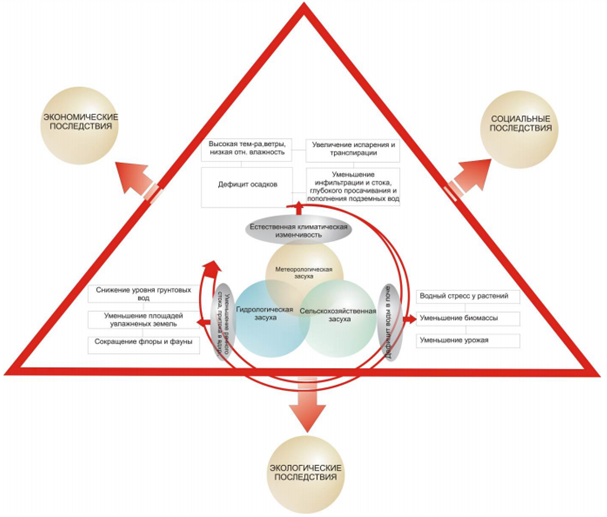
\includegraphics [scale=0.7] {drought_types}
	\caption{Виды засухи, их взаимодействие и влияние \cite{PROON2012}.}
	\label{img_drought_types}
\end{figure}

Засушливые явления отличаются друг от друга по трем основным характеристикам: интенсивность, продолжительность, пространственный охват. 

Они сопровождается высокими температурами воздуха при малом количестве осадков. Температура, равная и выше 35 \textdegree С, наблюдается в стране, преимущественно, с конца мая по октябрь, хотя в отдельные годы, особенно на юге, жара начинается уже в апреле, а иногда даже в марте. Пик числа жарких дней приходится в среднем на июль, хотя в отдельные годы наблюдается и в августе месяце. Почвенная засуха наблюдается в пустыне Кызылкум и Центральной Фергане с конца марта или начала апреля. На равнинных территориях этот процесс начинается с первой декады апреля, а в восточной части страны и предгорьях - в июле месяце \cite{Chub2001, Chub2007}.

В предгорной зоне Узбекистана очень сильная засуха (SPI < -50) весной наблюдается редко - 1--3 раза за 100 лет, а засуха с дефицитом сезонных сумм осадков в 20--25\% (SPI < -20) является достаточно регулярным явлением, наблюдаемым с вероятностью 30\%. 
В зоне пустынь и полупустынь очень сильная весенняя засуха (SPI < -50) проявляется в среднем 1 раз в 10 лет. Число дней с атмосферной засухой на большей части равнинных ландшафтов не превышает 30 дней, на юге эта цифра возрастает до 30-50 дней, и в Каршинской степи достигает 50-70 дней \cite{Chub2007}. Сравнительный анализ значений индекса осадков SPI с индексом по снегозапасам для зимних осадков (январь-март) и стоком за вегетацию в бассейнах рек Ахангаран и Пскем подтверждает определенную синхронность их колебаний.

В последнее десятилетие наблюдается увеличение периодичности засухи - она становится более частой в летний и осенний сезоны, особенно в низовьях реки Амударьи и в окрестностях Аральского моря. В 80-х и 90-х годах прошлого столетия засуха наблюдалась в среднем 2 раза в 10 лет. За период 2000 -- 2012 гг экстремальная засуха была зафиксирована 4 раза - в 2000, 2001, 2008 и 2011 годах []. 

Суровая засуха 2000-2001 годов стала особо опасной по масштабам распространения, воздействиям и последствиям для сельского и водного хозяйства и других секторов экономики, окружающей среды и сельского населения. Ответные меры и уроки, полученные в период суровой засухи 2000-2001гг, были детально изучены всеми заинтересованными учреждениями и международными организациями \cite{Zasuha2005}.
По данным \cite{Agalceva2012} 2011 год стал экстремально засушливым годом для Узбекистана за прошедшие 60 лет. Практически по всей территории Узбекистана наблюдается увеличение числа дней с температурой 40 \textdegree С и более, по сравнению с среднемноголетними данными. Это подтверждает тренд долгосрочных изменений показателей метеорологической и гидрологической засухи в бассейне реки Кашкадарья (пост Варганза) за период 1960-2011 гг. На значительной части Узбекистана было зафиксировано число засушливых дней с дефицитом влажности воздуха E $\geq$ 50 гПа в пределах нормы и выше нормы. Согласно прогнозным оценкам подобные тенденции, станут более широко распространенными \cite{NatSoob2, NatSoob3}.

Участившиеся засухи причиняют огромный ущерб и несут угрозу для жизнедеятельности населения, безопасности и социально-экономического развития страны. Воздействия засухи затрагивают практически все сектора экономики и сегменты населения, и представляют реальную угрозу благосостоянию населения и продовольственной безопасности Республики.
Биофизические воздействия. Из-за природно-географических и климатических особенностей Узбекистан очень чувствителен к деградации природной среды, особенно в связи с хрупкостью аридных систем и ограниченностью водных ресурсов. 
Засухи снижают буферные и фильтрационные свойства почвы, ее роль в гидрологическом и азотном циклах, способность обеспечить среду обитания для микроорганизмов и поддерживать биоразнообразие. Потеря растительного покрова вызывает сильную эрозию почв, уплотнение структуры почв и потерю здоровья почв. Засуха усиливает мобилизацию и аккумуляцию солей в верхних горизонтах почв и увеличивает засоление и деградацию земли во времени и в пространстве \cite{Zasuha2013}.

Засуха снижает доступность пастбищ для домашнего скота и диких животных. Численность диких пастбищ также имеет тенденцию к сокращению в связи с миграцией животных и потерей биомассы, которые возникают от недостатка воды. 
Более частые атмосферные засухи, с экстремально высокими температурами и низкой влажностью, особенно опасны в сочетании с недостатком воды для орошаемого земледелия - происходит угнетение посевов, недобор и/или гибель урожая на больших территориях. Например, потери урожая зерновых культур в годы суровой засухи 2000-2001 составили 14-17\%, а по другим культурам - в среднем от 45- 52\% до 75\% (низовья Амударьи).

Фактически, засуха 2000-2001гг формировалась постепенно, была необычной из-за дефицита осадков в сочетании с высокими уровнями испарения, вызванными жаркой погодой в течение нескольких лет. Уровни осадков достигли лишь 40\%-60\% от нормы, что привело к чрезвычайному сокращению речного стока (на 35\%-40\% от среднего уровня). Речной сток в низовье р. Амударьи был рекордно низким - Каракалпакстан получил лишь 20-30\% от потребности воды в период вегетации 2000 года. Гидрологические и социально-экономические эффекты засухи ощущались до конца 2003 года, в то время как осадки и сельскохозяйственное производство возвратились в норму в большинстве районов в 2002 г. \cite{Zasuha2013}.

Засуха 2000-2001гг. явилась катализатором процессов опустынивания и деградации окружающей среды, особенно в низовьях реки Амударьи. К концу 2001 г. практически полностью пересохли озерные системы озер и ветланды в северной части Каракалпакстана, площадью около 160 тыс.га. В результате исчезновения водно-болотной среды обитания в Красную книгу Узбекистана в 2000-2001 гг. было занесено 46 видов. Уровень подземных вод в районах охваченных засухой снизился до 10-15 метров, в результате большинство артезианских колодцев оказались бесполезными. Ухудшилось качество воды - минерализация воды в реки Амударья (Каракалпакстан) составила 0.85-2.1 г/л, жесткость достигала 17 мг/л.

Социально-экономические воздействия. Экономические и социальные воздействия засухи являются существенными и многоплановыми и проявляются, в частности, в сокращении сельскохозяйственной продукции и увеличении масштабов малообеспеченности, нехватке продовольствия и воды для хозяйственно-бытовых и питьевых нужд, росте детской смертности и обострении социальных конфликтов и/или усилении экологической миграции.

Нарушение динамики и производительности услуг напрямую влияют на продуктивность растениеводства, животноводства и рыбоводства и отвлекает значительные финансовые ресурсы страны на ликвидацию последствий в пострадавших регионах и т.д. Полный анализ издержек усложнен неопределенностью границ, поэтому во многих случаях зачастую не учитываются косвенные потери, издержки за пределами затрагиваемого района или соотношение издержек в случае осуществления действий и в случае бездействия. Соответственно, потенциальные экономические выгоды сокращения масштабов засух часто сильно недооцениваются.

Анализ последствий засухи 2000-2001 гг., по Каракалпакстану и Хорезмской области показывает, что наиболее драматические снижения в сельскохозяйственном производстве происходили вследствие недостаточности планирования, прогнозирования и контроля над водными ресурсами на региональном, республиканском и местном уровнях, что привело к уменьшению водоподачи на 20-30\% и 35-80\% соответственно по сравнению с утвержденным лимитом на воду. Как следствие, около 200 тыс. хозяйств (1.000.000 человек) потеряли урожаи.

По данным регионального обзора убытки, вызванные сельскохозяйственной засухой 2000-2001гг. в Узбекистане составили 130 млн. долларов США или 2.4\% от с/х ВВП. По другим источникам \cite{Zasuha2013}, величина ущерба оценивается в размере 38-40 млн. долларов США.
Значительные потери отмечались в животноводческом секторе. Чрезмерно стравленные пастбища вокруг сельских населенных пунктов и кишлаков были полностью лишены водоснабжения. В результате, заготовка кормовых трав сократилась более, чем на половину. В некоторых затронутых районах Каракалпакстана, засуха вынудила фермеров продать значительную часть своего стада или сельскохозяйственного оборудования.

Потеря биопродуктивности биоценозов и водной биоты водоемов в результате критических изменений гидрорежима в дельте Амударьи в годы засухи привели к тотальной гибели популяций промысловых рыб региона, подрыву ресурсной базы и краху рыбного хозяйства. За всю историю рыболовства наименьший улов рыбы в дельте Амударьи был в последующие после засухи годы: 131.6 тонн (2003) и 239.2 тонны (2004). На грани банкротства оказалось 51 фермерских хозяйств Каракалпакстана, арендовавшие свыше 60 тыс. га озерных систем.

Помимо экономического ущерба, засуха оказала значительные социальные эффекты. Наиболее сильно пострадавшему населению (порядка 600 000 человек) потребовались продукты питания, питьевая вода, помощь в поставке сельхозресурсов, затраты на которые в 2000-2001 гг. в Узбекистане составили 19 млн. долларов США. Оценки показали, что 2001 года порядка 79 000 хозяйств в Каракалпакстане и 21 000 в Хорезме остались без работы. Увеличилась миграция за пределы Узбекистана (в основном из Каракалпакстана в Казахстан) в поисках лучших жизненных условий. 
Недостаток воды для полива и/или ее низкое качество приводит к тому, что на всех уровнях (особенно домохозяйств и фермеров) происходит поиск адекватных стратегий преодоления нехватки воды. Это поиск дополнительных источников воды, меры по водосбережению и улучшению ирригационной и дренажной сети, и другие виды деятельности. Все они требуют труда, энергии, материальных затрат и навыков, но также влекут за собой социальные и экологические риски. В большинстве случаев, не имея альтернативных источников воды, усилия фермеров и дехкан сводятся к отбору воды из коллекторов и/или подземных вод, что вызывает засоление и деградацию земли, и связанные с этим ущербы урожая и, другие экономические и экологические ущербы. Ненадежная подача воды на орошение и ухудшение земли (особенно, засоление и заболачивание участков) усугубляют проблемы малообеспеченности.

В последнее десятилетие инвестиции и вклады государства при поддержке международных организаций в водный и сельскохозяйственный сектора и рост занятости в несельскохозяйствен¬ной сфере, способствовали диверсификации сельского хозяйства, предоставляя фермерам и пастухам более широкие возможности для преодоления засухи и смягчения ее эффектов. Тем не менее, большинству фермеров не хватало средств и знаний, чтобы воспользоваться преимуществами доступа к информации и смягчающим мерам, а развитие занятости в несельскохозяйственном секторе значительно отставало от других инициатив в области сельскохозяйственного развития.

Согласно данным опроса общественности, проведенного Центром социологических и рыночных исследованиям «Эксперт Фикри», в районах, пострадавших от засухи 2000-2001 гг., в результате недостатка воды участились случаи диареи и кишечных расстройств, острых респираторных заболеваний и болезней, связанных с употреблением некачественной воды. 

Меры по смягчению последствий засухи, как правило, осуществляются в порядке реагирования с точки зрения управления действиями в кризисных ситуациях и, как известно, такое реагирование не приносит должного результата. В годы засух создается специальная Комиссия с привлечением всех ключевых министерств и ведомств, которая разрабатывает меры и действия по смягчению последствий засухи \cite{Zasuha2013}. 

\subsection{Мониторинг и оценка}
Выбор индикаторов засухи является одним из главных вопросов организации мониторинга и оценки засух. 
Основу мониторинга засухи составляют данные наблюдений за метеорологическими, гидрологическими и агрометеорологическими параметрами - характеризующими частоту, пространственное распределение и продолжительность засух, которые проводит Узгидромет. 
Сеть наземных наблюдений включает: 
\begin{enumerate}
	\item 130 – гидрологических постов; 
	\item 79 – метеорологических станций на ежедневной и десятидневной основе; 
	\item агрометеорологические наблюдения, которые ведутся на 61 станции и 30 постах; 
	\item наблюдения за состоянием снежного покрова на 12 наземных и 138 аэровизуальных пунктах. 
\end{enumerate}

Помимо наземного мониторинга для оценки и предупреждения засух применяются данные дистанционного зондирования земли.
Перечень данных необходимых для предупреждения и оценки засух.

\begin{enumerate}
	\item Метеорологическая засуха 

	\begin{enumerate}
		\item Временной ряд климатических показателей, влияющих на засуху: температура, влажность воздуха, потенциальная эвапотранспирация;
		\item Частота засушливых лет;
		\item Прогнозируемая частота засушливых лет при различных сценариях климатических изменений;
		\item Количество и состояние метеорологических станций.
	\end{enumerate}

	\item Гидрологическая засуха

	\begin{enumerate}
		\item Временной ряд данных о площади и объеме поверхностных вод, сборе, подземных водных ресурсах, инфильтрации и изменчивости водного горизонта;
		\item Временной ряд данных о водном балансе: планируемые и фактические заборы воды различными отраслями; процентная доля ВВП и занятости в различных секторах;
		\item Временной ряд данные по областям и районам по орошаемым и не орошаемым участкам (планируемый и фактический), водозаборы для этих участков, и потери воды в магистральных каналах и в межхозяйственных и внутрихозяйственных ирригационных системах;
		\item Частота гидрологической засухи (разной степени) в разных районах;
		\item Количество и состояние станций по мониторингу стока и снежного покрова
		\item Меры по водоуправлению, за последние 10-15 лет, на межгосударственном и местном уровнях, такие как проведение переговоров, регулирование водохранилищ, сокращение лимитов, планы по водопользованию, ротации и т.д.;
		\item Минимальная/максимальная потребность гидроэнергетического потока и наличие водных ресурсов; процент электричества, генерируемого гидроэнергетикой;
		\item Максимальная/минимальная потребность воды для рыбного хозяйства и наличие водных ресурсов; оцениваемые потери;
		\item Максимальная/минимальная потребность воды для ветландов и экологическая сбалансированность рек и наличие водных ресурсов;
		\item Воздействие гидрологической засухи на опустынивание;
		\item Уязвимость.
	\end{enumerate}

	\item Сельскохозяйственная засуха

	\begin{enumerate}
		\item Количество и состояние агрометеорологических станций;
		\item Зависимость урожая от погоды (орошаемые и неорошаемые угодья, пастбища);
		\item Качество почв в основных агроэкологических зонах; классификация состава, содержание гумуса, способность почвы удерживать влагу, бонитет;
		\item Процентная доля орошаемых и неорошаемых земель в ВВП и т.п.;
		\item Диверсификация производства (растениеводство, животноводство, агролесоводство и т.п.);
		\item Процентная доля посевных земель, садов и пастбищных орошаемых ресурсов;
		\item Процент засоленных почв различной категории;
		\item Реагирование урожая на засоление воды и/или почвы, при различных культурах;
		\item Скотоемкость пастбища, процент деградированных пастбищ, максимальный погектарный выпас скота по регионам;
		\item Структуры земледелия и оцененные потребности в воде;
		\item Внутрихозяйственные агротехнические меры, предпринимаемые во врем и после засухи;
		\item Урожайность культур по районам;
		\item Ущерб от засух
	\end{enumerate}
\end{enumerate}

\subsection{Подходы и методы оценки засухи. Предупреждения засухи}

Засухи из опасных гидрометеорологических явлений являются наиболее дорого обходящихся природных опасных явлений, т.к оказывают значительные воздействия одновременно на многие сектора экономики и население. Но медленное наступление засухи дает потенциальную возможность к ее управлению. 

Управление засухой должно учитывать постоянное наблюдение и оценку состояния за определенными показателями/индикаторами засухи, оценку риска засухи - факторы воздействий, уязвимости и последствий, наличие системы заблаговременного предупреждения о засухе, а также обеспечение готовности и смягчение последствий. Важно, чтобы показатели или индексы засушливости достоверно отражали и представляли воздействия, которые проявляются во время засухи.

Другими словами, системы заблаговременного предупреждения о засухе (СЗПЗ), как правило, преследуют цель отследить и оценить климатические и гидрологические условия и тренды, а также водообеспеченность и предоставить соответствующую информацию о них. Их главная задача заключается в предоставлении своевременной информации заранее или во время начального этапа наступления засухи с целью стимулирования незамедлительных действий, опираясь на план управления рисками засухи, с тем чтобы снизить ее потенциальные воздействия. 
Многочисленные показатели засухи должны контролироваться регулярно, чтобы определить степень засухи и возможные последствия, с применением индексов для предупреждения и оценки засухи.
Для мониторинга/наблюдения и оценки засухи, необходим комплексный подход из-за сложного характера засух. 

В силу того, что проблему исследований и борьбы с засухой, как уже говорилось, необходимо решать комплексно, начиная с изучения количественных критериев и характеристик в зависимости от географической среды, времени года и объектов воздействий \cite{Zasuha2013, OON2010}.

Поскольку засухи являются следствием климатических и погодных условий, а также высокой уязвимости инфраструктуры и населения, изучение засухи необходимо проводить на основе метеорологических параметров (температура воздуха, дефицит влажности воздуха, осадки, влагозапасы почвы), которые в той или иной мере связаны между собой. 
Индексами засухи могут быть различные комбинации гидрометеорологических и социоэкономических характеристик и степени уязвимости.

Существуют различные подходы при идентификации трех вышеуказанных видов засухи.
Как уже отмечалось метеорологическая засуха характеризуется дисбалансом между осадками и испарением, который отмечается на отдельных территориях в различные сезоны года. При метеорологическом подходе в качестве индексов засухи рассматриваются значения метеорологических элементов, таких как температура воздуха, осадки, влажность воздуха и почвы, а также различные показатели, представляющие собой комбинации этих характеристик за определенные периоды времени.
Вопросы мониторинга, предупреждения, оценки засухи и смягчения ее последствий изучается во всем мире давно и основательно, т.к. это явление наблюдается во всех регионах Земли. Всемирной метеорологической организацией (ВМО) разработаны Руководящие документы по выбору индикаторов, методологии по оценки общепринятых показателей, которые будут проанализированы в данном разделе.
Для выбора индексов и показателей необходимо: (1) для однозначного трактования определиться в некоторых понятиях; (2) определить критерии отбора индикаторов; (3) рассмотреть подходы для мониторинга засух и для индикаторов заблаговременного предупреждения.
Определения.

Индикатор – это количественный или качественный показатель, им может быть какой-либо параметр, индекс, коэффициент и т.д., характеризующий изменения или фиксацию процесса и позволяющий дать оценку результатов деятельности процесса \cite{Rakhmatova2017}.
Показатели представляют собой переменные или параметры, используемые для описания засушливых условий. Примерами являются количество осадков, температура, речной сток, уровень грунтовых вод и воды в водохранилищах, почвенная влага и снежный покров \cite{Handbook2016}.

Индексы, представляют собой полученные путем расчетов численные представления интенсивности засухи, оцененные с использованием климатических и гидрометеорологических входных параметров, включая показатели, перечисленные выше. Они предназначены для оценки качественного состояния засушливости на данном ландшафте за конкретный период времени. Индексы могут использоваться для упрощения сложных соотношений и служить полезным средством для информирования самых различных аудиторий и пользователей. Индексы используются для количественной оценки интенсивности, района распространения, сроков и продолжительности явления засухи. Под интенсивностью понимается степень отклонения от нормального значения индекса. Может быть установлено пороговое значение интенсивности, для того чтобы определить, когда началась засуха, когда она закончилась, а также какой географический район подвергся ее воздействию. Районом распространения может быть географическая область, испытывающая влияние засушливых условий. Сроки и продолжительность определяются по приблизительным датам наступления и завершения засухи. Последствия определяется взаимосвязью между наступившим опасным явлением и подвергшимися воздействию элементами (люди, сельскохозяйственные угодья, водохранилища и запасы воды), а также уязвимостью этих элементов. Уязвимость может усугубляться предыдущими засухами, которые, например, повлекли за собой продажу производственных активов для удовлетворения первоочередных потребностей. Сроки засухи могут быть столь же важны, как и ее интенсивность, в определении воздействий и последствий засухи. Таким образом, индексы засушливости, в сочетании с дополнительной информацией о подвергшихся воздействию активах и их характеристиках уязвимости, обладают принципиально важным значением для отслеживания и предвидения связанных с засушливостью воздействий и последствий \cite{Handbook2016}.

Триггеры — это конкретные значения показателя или индекса, которые служат основанием для инициирования и/или завершения определенного уровня плана борьбы с засухой и соответствующих мер реагирования в контексте управления в чрезвычайных ситуациях и смягчения их последствий. Другими словами, они являются пусковым механизмом для действий и предусматривают систему ответственности, определяющую, кем, какие и когда должны предприниматься действия. Крайне важно наличие полного перечня триггеров для показателей и индексов, которые должны соответствовать плану мероприятий, служащему основанием для скоординированного набора мер отдельных учреждений или министерств. В отсутствие подобного соответствия существует вероятность значительных задержек с принятием мер при наступлении засухи в районе или регионе \cite{Handbook2016}.

\subsection{Критерии отбора}
Учитывая опыт международных и национальных практик, на основе гармонизации критериев к индикаторам и требований КБО ООН, выбор индикаторов должен основываться на Принципах Парадигмы развития засушливых земель (DDP – Drylands Development Paradigm), критериях SMART и DPSIR, согласно которым индикаторы должны \cite{Rakhmatova2017}: 

\begin{enumerate}
	\item быть достоверными, просто и наглядно описывать реальную ситуацию и ограничены в количестве показателей.
	\item направлены на оценку изменяющейся ситуации, и иметь количественную характеристику.
	\item иметь необходимые временные ряды соответствующих данных для оценки прогресса и отражения тенденций
	\item соответствовать ключевым аспектам обязательств по Конвенции.
	\item быть понятными ( Выбор, расчеты и значения ) даже не специалистам.
	\item быть удобным для анализа и принятия решений по эффективному выполнению обязательств КБО ООН.
	\item быть масштабируемым, т.е. должны быть данные для оценки на выбранном масштабе (район, область, страна).
	\item представлять собой интегрированную информацию, которая могла бы быть использована в долгосрочном плане для принятия решений.
\end{enumerate}

Схема разработкии индикаторов должна основываться на следующих действиях: 

\begin{enumerate}
	\item анализ информации о международных и национальных практиках и подходах для оценки ОДЗЗ;
	\item проведение инвентаризации существующей информации в стране - сбор существующей доступной информации;
	\item анализ ситуации ОДЗЗ в стране;
	\item разработку предварительного перечня индикаторов на основе полученной информации. 
\end{enumerate}

При выборе использования показателей и индексов для определенной ситуации необходимо проанализировать их на соответствие следующим параметрам \cite{Handbook2016}:

\begin{enumerate}
	\item Своевременное обнаружение/идентификация засухи 
	\item Чувствительность к климату, пространству и времени для определения начала и завершения засухи
	\item Уровень интенсивности для отражения воздействий, происходящих на местах в конкретной точке или регионе
	\item Способность определения периодов наступления засухи и ее окончания 
	\item Применение комплексных/гибридных показателей для учета многофакторности входных параметров
	\item Оценка доступности и устойчивости (наличие временных рядов у конкретного источника данных, имеющих способность отразить ретроспективу
	\item Доступность в реализации на практике показателя/индекса (наличие людских, технических, временных ресурсов
\end{enumerate}

\subsection{Методы и подходы к выбору показателя/индикатора/индекса}

На сегодняшний день существует три основных метода для мониторинга и заблаговременных предупреждений/оценок \cite{Handbook2016}:

\begin{enumerate}
	\item использование единого показателя или индекса; 
	\item использование множества показателей или индексов; 
	\item использование комплексных или гибридных показателей.
\end{enumerate}

В течение нескольких десятилетий появляется тип комплексных показателей Особый акцент сегодня делается на использование гибридных показателей, так называемый гибридный, основанный на совмещении различных показателей и индексов, будь то взвешенные или не взвешенные показатели, либо полученные на основе моделирования. Идея заключается в том, чтобы использовать сильные стороны различных входных параметров, сохранив при этом единый и простой источник для лиц, принимающих решения и ответственных за выработку политики и мер по смягчению последствий засухи.

Актуальными являются вопросы картирования явления, для оценки подверженности влияния засухи на население, сектора экономики и экосистемы. В решении данного вопроса используются геоинформационные системы и применение дистанционных методов зондирования Земли.
Индексы метеорологической засухи

Индексы, расчет значений которых основан в основном на экспериментальных данных мировой сети метеорологических станций по осадкам, классифицируются как индексы метеорологической засухи. Этот тип индексов засухи был одним из первых рассмотрен в научных и прикладных исследованиях. В качестве примера такого типа индексов засухи можно отметить:

\begin{enumerate}
	\item Индекс аномалии осадков;
	\item Индекс засухи Bhalme и Mooley
	\item Стандартизированный Индекс Аномалии;
	\item Индекс засушливости (ариадности) Palfai , разработанный и применяемый в основном в Венгрии;
	\item Индекс интенсивности засухи , часто используемый в Великобритании;
	\item Стандартизированный индекс осадков , наиболее популярный;
	\item Эффективный индекс засухи рассматривающий эффективность осадков.
\end{enumerate}

\subsection{Гидрологические индексы засухи}

Другим классом индексов засухи являются индексы, разработанные для области гидрологии:

\begin{enumerate}
	\item Базовый (основной) индекс потока;
	\item Региональный индекс дефицита руслового стока ;
	\item Гидрологический индекс засухи Палмера;
	\item Индекс запаса поверхностных вод;
	\item Индекс регенерации засухи ;
\end{enumerate}

В классической гидрологии для определения состояния засухи, как правило, используется анализ руслового стока или уровня грунтовых вод.

Гидрологическая засуха анализирует в терминах дефицита объема руслового стока, который рассматривается по сезону или более длинным периодам времени, либо в региональном контексте.
Наиболее часто прикладная количественная четкость гидрологической засухи основана на определении порогового значения q0, ниже которого речной сток или уровень подземных вод рассматривают как засуха (также называется в литературе нижним значением потока по периоду). Метод порогового уровня в целом рассматривает значения руслового стока (уровня подземных вод) ниже или выше данного порога и был первоначально назван методом кроссирующей теории. Метод важен для анализа накопления/сброса объема воды в резервуарах и связан с гидрологическим расчетом и операциями по заполнению систем водохранилищ. Важные области использования – гидроэнергетика, сельское хозяйство, системы водоснабжения и ирригации.

\subsection{Индексы сельскохозяйственной засухи}

Для мониторинга и анализа влияния засухи на сельскохозяйственное производство разработаны специализированные индексы сельскохозяйственной засухи, такие как:

\begin{enumerate}
	\item Индекс увлажненности урожая;
	\item Индекс засухи влажности почвы;
	\item Специальный индекс засухи урожая;
	\item Индекс дефицита влажности почвы;
	\item Индекс дефицита эвапотранспирации;
	\item DTx индекс;
\end{enumerate}

Определение сельскохозяйственных индексов включает ежедневные значения температуры и осадков, фактическую и потенциальную эвапотранспирации и ряд других параметров для заданных временных интервалов.
Одной из последних разработок в области сельскохозяйственных индексов засухи – Soil MoistureDeficitIndex. Индекс разработан на основе модели водного баланса – гидрологической модели SWAT (Soil and Assessment Tool). Основные компоненты модели включают погоду, гидрологию, температуру почвы, состояние растений, пестициды, удобрения и землеустройство.

\subsection{Индексы, основанные на данных дистанционного зондирования}

Наблюдения из космоса со спутников за параметрами и характеристиками поверхности Земли проводится с 1980 годов, с использованием чувствительных датчиков. Полученные данные открывают новые возможности мониторинга и контроля засухи. Новые технологии учитывают отклонение в пространственной информации для глобального или регионального покрытия с высокой разрешающей способностью.

К данному классу индексов засухи относятся:

\begin{enumerate}
	\item Normalized Difference Vegetation Index, ( NDVI, 1979);
	\item Vegetation Condition Index, ( VCI, 1990);
	\item Temperature Condition Index, (TCI, 1995);
	\item Normalized Difference Temperature Index,( NDTI, 1998);
	\item Standardized Vegetation Index, (SVI,2002);
	\item Vegetation Health Index, (VHI, 1997, 2000);
	\item Vegetation Index/Temperature Trapeziod (VITT,1994);
	\item Vegetation Temperature Condition Index (VTCI, 2004);
	\item Temperature Vegetation Dryness Index (TVDI,2002);
	\item Vegetation Condition Albedo Drought Index (VCDAI, 2007);
	\item Perpendicular Drought Index (PDI, 2007);
	\item Modified Perpendicular Drought Index (MPDI, 2007);
	\item Multi-Band Drought Index (NMDI, 2007);
	\item Remote Sensing Drought Risk Index (RDRI, 2008);
\end{enumerate}

Вегетационные индексы (NDVI, VCI, SVI, и др.) обычно используют для определения состояния растительности. Индексы являются линейными или дробно-линейными комбинациями двух спектральных каналов: 06,-0,7 мкм (красный диапазон спектра) и 0,8-0,9 мкм (ближний ИК диапазон спектра). Выбор спектральных каналов обусловлен тем, что в красном диапазоне спектра растительность имеет наименьшее отражение, а в ближнем ИК-диапазоне спектра – самое высокое отражение по сравнению с другими природными объектами. Другими словами, для растительности c нормальным развитием характерно падение спектральной кривой в красном диапазоне и резкий подъем в ближнем ИК-диапазоне.
Индексы основанные на данных дистанционного зондирования в тепловом диапазоне ( TCI, TVDI, VITT и др.) позволяют получить оценку температурного режима земной поверхности, влажности почвы, эвапотранспирацию и ряд других параметров.

\subsection{Индексы засухи используемые на территории СНГ}

В республиках СНГ, как правило, для определения характеристик засухи и влажности почв используются следующие индексы:

\begin{enumerate}
	\item Индекс Педя;
	\item Гидротермический коэффициент Селянинова;
	\item Индекс сухости; 
	\item Коэффициент увлажнения;
\end{enumerate}

Приведенные индексы представляют собой полуэмпирические величины, определяемые на основе метеорологических данных сети станций
Анализ используемых индексов показывает, что все они не являются универсальными. Наиболее многочисленная группа индексов выражается через осадки, поскольку основной первопричиной любой засухи служит их недостаток. 
Ниже приведены некоторые методы оценки, применение которых возможно условиях Узбекистана.
Самый распространенный индекс засухи – стандартизированный индекс осадков \cite{Handbook2016, WMO1090}:

\begin{equation}\label{eq_1.1}
\begin{aligned}
	SPI = [(p-\bar{p})/\bar{p}] \times 100\%
\end{aligned}
\end{equation}

где $p$ – наблюдаемое количество осадков, $\bar{p}$ – их среднее значение. 
Широкое применение этот показатель получил благодаря простоте его вычисления и доступности исходных данных для этой цели. Кроме того, используя этот показатель, можно установить начало и окончание избыточно влажных, засушливых и сухих периодов, а также проводить районирование территории по этому фактору.

Например, анализ стандартизованного индекса весенних сумм осадков (март- май), вычисленного для станций предгорной зоны (Ташкент, Фергана), низовьев Амударьи (Ургенч) и зоны пустынь (Тамды) показал, что для предгорной зоны Узбекистана очень сильная засуха (SPI<-50) весной наблюдается редко (1-3 раза за 100 лет), а засуха с дефицитом сезонных сумм осадков в 20-25\% (SPI<-20) является достаточно регулярным явлением, наблюдаемым с вероятностью 30\% \cite{Myagkov2004}.

Известно, что для рек со снеговым и снегово-ледниковым типом питания водность рек определяется накоплением снега в горах в зимний период. Поэтому целесообразно использовать накопление снега в горах в качестве критерия (индекса) водности года.

Были использованы следующие две формулы для расчета индексов по указанному показателю:
\begin{equation}\label{eq_1.2}
\begin{aligned}
S_W = [(W-\bar{W})/\bar{W}]
S_W = [W/\bar{W}]
\end{aligned}
\end{equation}

где $W$, $\bar{W}$ -- снегозапасы за определенный срок (конец января, конец февраля и т.п.) и средние многолетние значения снегозапасов соответственно.

Во многих литературных источниках используют коэффициенты увлажнения, представляющие собой отношение годовых сумм осадков к испаряемости.
В качестве простого индекса аридности климата рекомендовано использовать годовую сумму осадков. Согласно этому критерию считается, что абсолютно аридные – территории с годовым количеством осадков менее 50мм, к аридной зоне относятся территории с годовым количеством осадков менее 250мм, полуаридной – от 250 до 450мм.
Очевидно, что предупреждение о засухе, ее интенсивности и продолжительности представляет большой интерес для широкого круга специалистов и различных слоев населения.

Исследования в области прогнозирования экстремальных метеорологических явлений (метеорологической засухи) являются одной из самых сложных и актуальных проблем мировой прогностической науки и практики. Очевидно, что решение этих вопросов будет способствовать если не ликвидации, то, по крайней мере, сглаживанию неблагоприятных последствий погодных аномалий, позволит судить о степени риска принятия конкретной стратегии в том или ином районе \cite{Agaltseva2004}.

Проблема предупреждения засухи тесно связана с проблемой долгосрочного прогноза температуры и осадков. Несмотря на многочисленные усилия, успешность сверхдолгосрочного (год и более) предупреждения засух невысока. Успешность месячных и сезонных прогнозов аномалий температуры и осадков несколько выше, но также недостаточна. Особенные трудности при долгосрочном прогнозировании возникают в континентальных районах умеренных широтах, где велика естественная изменчивость температуры и осадков, что характерно и для региона Средней Азии. В засушливых районах отмечается повышенная повторяемость аномалий осадков ниже нормы, т. е. возникает проблема прогноза редких явлений.

Другое направление долгосрочного прогнозирования связано с использованием статистических методов, которые позволяют находить общие закономерности формирования погодных условий на длительные периоды времени.

В настоящее время в практике Узгидромета используют статистические методы прогноза на сезон в качестве консультативных, официальный метод долгосрочного прогноза – синоптический (подбор годов-аналогов).

Успешность подобного рода месячных и сезонных прогнозов температуры и осадков во всех регионах мира недостаточно высока. Разработки в области долгосрочных прогнозов являются одними из первоочередных задач ВМО, наиболее перспективным направлением является использование глобальных гидродинамических моделей общей циркуляции (атмосферы и океана). Такие исследования и эксперименты ведутся в ведущих мировых метеорологических центрах.

В связи с вышесказанным, очевидно, что выбор и включение в систему различных индексов засухи имеет большое значение для снижения неопределенности при решении задачи раннего предупреждения засухи.

Для территории Узбекистана в качестве показателя интенсивности атмосферной засухи принята следующая шкала значений дневного дефицита влажности воздуха (таблица\ref{tb_atm_drouth}) и число дней с температурой выше 40 \textdegree C, по этим показателям составляются карты \cite{Chub2007}.

\begin{table}[!tb]
	\centering
	\caption{Показатели атмосферной засухи (дневной дефицит влажности воздуха, гПа)}\label{tb_atm_drouth}
	\begin{DoubleSpace}
	\begin{tabular}{| c | c | c | c |}
		\hline
		\hline
		50--60 гПа & 61-70 гПа & 71--80 гПа & >80 гПа \\ 

		\hline

		Слабая & Средняя & Сильная & Очень сильная \\ 

		\hline
		\hline
	\end{tabular}
	\end{DoubleSpace}
\end{table}

В качестве показателя гидрологической засухи для условий Узбекистана приняты: обеспеченность стока воды за вегетационный период (апрель-сентябрь) (таблица 2) и величины запасов воды в снежном покрове в горах на конец февраля и марта. Последний показатель используется при прогнозировании гидрологической засухи, когда в конце марта составляется прогноз водности вегетационного периода карты \cite{Chub2007}.

\begin{table}[!tb]
	\centering
	\caption{Гидрологический индекс засухи}\label{tb_atm_drouth}
	\begin{DoubleSpace}
		\begin{tabular}{| l | c | c |}
			\hline
			\hline
			\multirow{2}{*}{Показатель} & \multicolumn{2}{c|}{Засуха} \\ 
			\cmidrule(l){2-3}
			& Умеренная & Сильная \\
			
			\hline
			
			Обеспеченность вегетационного стока, P\% & 80\% < P < 95\% & P > 95\% \\ 

			\hline

			Cнегозапасы на конец февраля (расчет), $S_W$ & 80\% < - 0,2 & < -0,4 \\ 
			
			\hline
			\hline
		\end{tabular}
	\end{DoubleSpace}
\end{table}

В качестве критерия почвенной засухи для пустынной зоны Узбекистана принято снижение запасов почвенной влаги в почвенном слое толщиной 0-2 см до 4 мм, для глинистых полупустынных почв – 10 мм карты \cite{Chub2007}.
Также в настоящее время используются Стандартизированный индекс осадков по отдельным станциям, Индекс засушливости, индекс засухи, основанный на оценке снегозапасов.

Обзор и систематизация данных, информации, и публикаций Узгидромета и других источников, позволили выявить разнообразие метеорологических и гидрологических и сельскохозяйственных индексов засухи, применяемых в стране для оценки особенностей и тенденций засухи. В монографии В.Е. Чуба \cite{Chub2007} проведена оценка применяемых индексов, которая подтверждает их приемлемость для условий Узбекистана.

Мониторинг метеорологической засухи осуществляется посредством оценки значений критериев метеорологической засухи, которые позволяют судить о масштабах и ее продолжительности.
Выбор и использование различных индексов засухи имеет большое значение для снижения неопределенности при решении задачи мониторинга засухи. 

Анализ показывает, что наиболее распространенными индексами засухи для условий Узбекистана являются дефицит влажности воздуха и стандартизированный индекс осадков (SPI) и индекс засушливости (S). Широкое применение показатель SPI получил благодаря простоте его вычисления и доступности исходных данных для этой цели. Его можно использовать для характеристики глубины засухи, с учетом ее продолжительности, а также проводить ранжирование территории по этому фактору. С точки зрения изменения климата наибольший интерес представляет индекс засушливости (S) по Д. А. Педя (индекс Сазонова). С помощью этого индекса (S) можно характеризовать условия влагообеспеченностии теплообеспеченности. 

\paragraph{Программы}

Всемирная метеорологическая организация имеет рад программ прямо или косвенно связанных с вопросами засухи \cite{Agalceva2012} (\url{http://www.wmo.int/pages/summary/prog_description_en.html}).
Программа Всемирной службы погоды (ПВСП). ПВСП нацелена на содействие в разработке, эксплуатации и совершенствовании всемирных систем наблюдения и обмену метеорологическими и релевантными наблюдениями, а также для создания и распространения продуктов анализов и прогнозирования, рекомендаций, предупреждений о неблагоприятной погоду. Мероприятия, осуществляемые в рамках этой Программы, предполагают гарантии о том, что страны-члены будут иметь доступ к необходимой информации, для предоставления данных пользователям о прогнозах и другие информационные услуги и продукты.
В задачи ПВСП входит планирование, организация и координация объектов, процедур и механизмов на глобальном и региональном уровнях, связанных с проектированием сетей наблюдения и связями, стандартизация методов, наблюдений и измерений, принципы использования управления данными, применение научно-технических средств для обеспечения, анализа и прогнозирования метеорологических систем, а также представление информации в форме и формате, понятном всем, независимо от языка. ПВСП является ключевой программой ВМО в предоставлении базовых данных, анализов, прогнозов и предупреждений странам-членам и другим программам ВМО и совместно с такими программами как Глобальная система наблюдений за климатом и Глобальная система наблюдений за океаном и с соответствующими международными организациями.

ПВСП уделяет первоочередное внимание мероприятиям по наращиванию потенциала для использования технических достижений в целях совершенствования компонентов ВСП, особенно в развивающихся странах, а также по систематическому мониторингу и совершенствованию операций ВСП.

ПВСП предусматривает разработку, внедрение, эксплуатацию и дальнейшее развитие следующих трех взаимосвязанных и все более интегрированных основных компонентов:

\begin{enumerate}
	\item Глобальная система наблюдений (ГСН), состоящая из объектов и механизмов для проведения метеорологических наблюдений (включая климатологические наблюдения) и других соответствующих экологических наблюдений на станциях на суше и в море, а также с самолетов, метеорологических экологических спутников и других платформ;
	\item Глобальная система электросвязи (ГСТ), состоящая из интегрированных сетей средств и служб электросвязи для быстрого и надежного сбора и распространения данных наблюдений и обрабатываемой информации;
	\item Глобальная система обработки данных и прогнозирования (ГСОДП), состоящая из всемирных, региональных специализированных и национальных метеорологических центров, которые обеспечивают качество, обработку данных, анализ и прогнозирование продуктов в широком диапазоне временных и пространственных масштабов.
\end{enumerate}

ПВСП включает три программы, которые дополняют и улучшают основные компоненты ВСП, а также обеспечивают значительный вклад и поддержку другим программам ВМО: 

\begin{enumerate}
	\item Программа «Инструменты и методы наблюдений» (ИМОП) улучшает качество и долгосрочную стабильность наблюдений и измерений метеорологических и связанных с ними переменных окружающей среды посредством деятельности по стандартизации, а также координации и поощрения использования эффективных методов и технологий для требования к оперативным и исследовательским приложениям;
	\item Программа действий по реагированию на чрезвычайные ситуации (ERA) помогает НМГС эффективно реагировать на крупномасштабные загрязнения атмосферы и чрезвычайные экологические ситуации в тесном сотрудничестве с другими соответствующими международными организациями;
	\item Программа ВМО по антарктической деятельности (ВМОАА) координирует внедрение и эксплуатацию базовых систем ВСП в Антарктике для удовлетворения потребностей в метеорологическом обслуживании, а также для мониторинга окружающей среды и исследований климата.
\end{enumerate}

Системы компонентов Всемирной службы погоды в основном управляются в соответствии с технической ответственностью Комиссии по основным системам (КОС), за исключением ИМОП, которая управляется с технической ответственностью Комиссии по приборам и методам наблюдений (КПМН).

ПВСП тесно сотрудничает с другими связанными с ней программами, в частности с Космической программой ВМО (WMO Space Programme (WMO SP)), которая способствует широкому доступу и использованию спутниковых данных и продуктов для погоды, климата, воды и связанных с ними приложений для решения вопросов в области окружающей среды во всех программах ВМО; 

Глобальная система электросвязи (ГСЭ) представляет собой интегрированную систему сетей передачи данных с управляемыми данными, двухточечных схем и спутниковых систем сбора и передачи данных, которые соединяют метеорологические центры посредством согласованных процедур и услуг. Он предоставляет услуги электросвязи для сбора и обмена данными наблюдений и распространения обрабатываемой информации из Глобальной системы обработки данных и прогнозирования (ГСОДП) и других соответствующих центров. ГСЭ эксплуатируются Национальными метеорологическими службами, национальными или международными спутниковыми агентствами или контрактными поставщиками коммерческих телекоммуникационных услуг. Обслуживание и совершенствование систем для обмена данными, продуктами и информацией, таким образом, облегчает доступ к информации, необходимой для подготовки анализов, прогнозов и предупреждений, исследовательской деятельности и других приложений, связанных с окружающей средой.

Глобальная система обработки данных и прогнозирования (ГСОДП) представляет собой функцию прогнозирования погоды, включая подготовку метеорологического и климатического анализа, прогнозов, специализированных продуктов прогнозирования и предупреждений, рекомендаций и предупреждений о суровой погоде для защиты жизни и собственности. ГСОДП включает сеть оперативных метеорологических центров, которые производят широкий спектр продуктов, прогнозов и предупреждений с численным прогнозом погоды (ЧПП), и является частью глобальной системы раннего предупреждения о метеорологических и экологических опасностях. Результаты ГСОДП необходимы НМГС и другим организациям-членам для их удовлетворения разнообразных потребностей включающих реагирование на чрезвычайные ситуации, обычные прогнозы погоды, контроль за воздушным движением, прогнозы окружающей среды, состояния и/или качества воздуха и т.д. ГСОДП направлен на предоставление все более значимых, надежных и гарантированных качеством продуктов, охватывающих диапазоны прогнозов от мгновенного до долгосрочного и от местного до глобального масштаба, совершенствования служб раннего предупреждения для смягчения метеорологических бедствий и эффективных рекомендаций для чрезвычайных ситуаций ответ на экологические катастрофы.

ГСОДП способствует сокращению риска бедствий путем внедрения новых научно-технических средств для улучшения прогнозирования опасных погодных явлений 

Программа поддержки Всемирной службы погоды (WWWDM) – разработка и координация форматов данных, коды, стандарты метаданных, необходимые для упорядоченного и эффективного общего управления метеорологическими данными и продуктами. Координация мониторинга операций ВСП для повышения доступности и качества данных и продуктов.

Программа инструментов и методов наблюдения (ПИМН) организует необходимые исследования, такие как интерактивные сопоставления приборов, калибровка для обеспечения требуемой точности и гарантий долгосрочной стабильность и функциональной совместимости систем наблюдений. Так же программа нацелена на разработку и публикацию технических руководств, методик наблюдения, стандартов и характеристик работы.

Деятельность по реагированию на чрезвычайные ситуации (ERA) – это программа по реагированию на чрезвычайные ситуации, осуществляемая в тесном сотрудничестве с Глобальной системой обработки данных и прогнозирования, помогает НМГС и другим соответствующим учреждениям, а также соответствующим международным организациям эффективно реагировать на экологические чрезвычайные ситуации, к примеру в результате ядерных аварий, извержений вулканов, химических аварий, дыма от крупных пожаров и других событий, которые требуют поддержки при атмосферном переносе и моделировании дисперсионного моделирования (ATM). 

Программа снижения риска бедствий (Disaster Risk Reduction Programme) Цель Программы заключается в оказании странам-членам помощи в обеспечении и предоставлении услуг, направленных на защиту жизней, средств к существованию и собственности, экономически эффективным, систематическим и устойчивым образом. Программа нацелена на содействие укреплению институционального потенциала в области предоставления метеорологического, гидрологического и климатического обслуживания и сотрудничества в области поддержки управления рисками стихийных бедствий в целях защиты жизни и имущества и содействия устойчивому развитию п стран-членов.

Реализация программы направлена на решение следующих задач: 

\begin{enumerate}
	\item разработка, совершенствование и устойчивость систем раннего предупреждения, в частности связанных с научными и техническими инфраструктурами, системами и возможностями для проведения исследований, наблюдения, обнаружения, прогнозирования и предупреждения опасных погодных, водных и климатических явлений;
	\item разработка, совершенствование и устойчивость стандартизованных баз данных о рисках и метаданных, систем, методов, инструментов и приложений современных технологий, таких как географические информационные системы для регистрации, анализа и предоставления информации об опасности для оценки рисков, секторального планирования, передачи рисков и других информированных принятие решения;
	\item разработка и предоставление предупреждений, специализированных прогнозов и других продуктов и услуг, которые являются своевременными, понятными для тех, кто подвергается риску и обусловленными требованиями процессов и операций по уменьшению опасности бедствий, связанных с социально-экономическими секторами;
	\item устойчивость и профилактика путем укрепления потенциала для лучшей интеграции продуктов и услуг метеорологии, гидрологии и климата в снижение риска бедствий во всех социально-экономических секторах, таких как планирование землепользования и проектирование инфраструктуры, а также непрерывное государственное образование и информационно-пропагандистские кампании;
	\item сотрудничество и налаживание партнерских отношений ВМО и НМГС на национальных, региональных и международных форумах пользователей, механизмов и структур для осуществления уменьшения опасности бедствий.
\end{enumerate}

Программа агрометеорологии ВМО (Agricultural Meteorology Programme (AgMP) \url{http://www.wmo.int/pages/prog/wcp/agm/agmp_en.php})

Цель AGMP заключается в оказании помощи странам-членам ВМО в предоставлении метеорологических и релевантных услуг для сельского хозяйства с целью содействия создания устойчивых и экономически жизнеспособных сельскохозяйственных систем.
Программа отражает в себе деятельность по засухе проводимой ВМО, т.к. сельскохозяйственный сектор наиболее уязвим к засухе.
Данная программа включает в себя методические документы (Руководство по агрометеорологической практике 2010 г.), публикации (брошюры, книги, отчеты, специальные статьи журналов. 

Руководство имеет следующие разделы:

\begin{enumerate}
	\item Сельскохозяйственные метеорологические элементы и их наблюдения
	\item Сельскохозяйственные метеорологические данные, их представление и статистический анализ
	\item Приложения дистанционного зондирования и ГИС в агрометеорологии
	\item Прогноз погоды и климата для сельского хозяйства
	\item Агрометеорологическое прогнозирование
	\item Оценка климатических и погодных рисков для сельскохозяйственного планирования
	\item Последствия изменения климата для сельского хозяйства
	\item Применение метеорологии к сельскому хозяйству
	\item Агрометеорология некоторых выбранных культур 
	\item хлопок, арахис, кукуруза, жемчужное просо, картофель, рис, сорго, пшеница
	\item Применение метеорологии к лесным и нелесным деревьям
	\item Погода и климат и производство животных
	\item Применение агрометеорологии к аквакультуре и рыболовству
	\item Агрометеорологические аспекты опустынивания
	\item Аэробиология
	\item Применение климатических ресурсов в горных районах
	\item Передача агроклиматологической информации, в том числе прогнозов, для сельскохозяйственных решений
\end{enumerate}

Программа имеет связь с Программой интегрированного управления засухой 
И Принятой совместно ВМО и КБО ООН Инициативой Национальная политика засухи. 
Программа интегрированного управления засухой (IDMP) работает с широким кругом партнеров с целью поддержки заинтересованных сторон на всех уровнях, предоставляя им руководство в области политики и управления посредством глобального согласованного формирования научной информации и обмена передовым опытом и знаниями для комплексного управления засухой. IDMP является вкладом в Глобальную рамочную основу для климатического обслуживания (ГОКО), особенно в отношении приоритетных областей ГОКО, связанных с уменьшением опасности бедствий, водой, сельским хозяйством и продовольственной безопасностью. Он, в частности, направлен на поддержку регионов и стран в разработке более активной политики засухи и совершенствовании механизмов прогнозирования \cite{Zasuha2005, vakbib1}.

\begin{enumerate}
	\item Понятие засухи
	\item Типы засухи
	\item Засуха в глобальном масштабе
	\item Засуха в региональном масштабе
	\item Засуха на национальном уровне
	\item Ситуативный анализ
	\item Индикаторы
	\item Методы распространения информации
	\item Мониторинг
	\item Прогноз/предупреждение
\end{enumerate}

           % Глава 1
\chapter{Длинное название главы, в которой мы смотрим на~примеры того, как будут верстаться изображения и~списки} \label{chapt2}

\section{Одиночное изображение} \label{sect2_1}

\begin{figure}[ht]
  \centering
  \includegraphics [scale=0.27] {latex}
  \caption{TeX.}
  \label{img:latex}
\end{figure}

\section{Длинное название параграфа, в котором мы узнаём как сделать две картинки с~общим номером и названием} \label{sect2_2}

А это две картинки под общим номером и названием:
\begin{figure}[ht]
  \begin{minipage}[ht]{0.49\linewidth}\centering
    \includegraphics[width=0.5\linewidth]{knuth1} \\ а)
  \end{minipage}
  \hfill
  \begin{minipage}[ht]{0.49\linewidth}\centering
    \includegraphics[width=0.5\linewidth]{knuth2} \\ б)
  \end{minipage}
  \caption{Очень длинная подпись к изображению,
      на котором представлены две фотографии Дональда Кнута}
  \label{img:knuth}
\end{figure}

Те~же~две картинки под~общим номером и~названием,
но с автоматизированной нумерацией подрисунков:
\begin{figure}[ht]
    {\centering
        \hfill
        \subbottom[List-of-Figures entry][Первый подрисунок\label{img:knuth_2_1}]{%
            \includegraphics[width=0.25\linewidth]{knuth1}}
        \hfill
        \subbottom[\label{img:knuth_2_2}]{%
            \includegraphics[width=0.25\linewidth]{knuth2}}
        \hfill
        \subbottom[Третий подрисунок]{%
            \includegraphics[width=0.3\linewidth]{example-image-c}}
        \hfill
    }
    \legend{Подрисуночный текст, описывающий обозначения, например. Согласно
    ГОСТ 2.105, пункт 4.3.1, располагается перед наименованием рисунка.}
    \caption[Этот текст попадает в названия рисунков в списке рисунков]{Очень
    длинная подпись к второму изображению, на~котором представлены две
    фотографии Дональда Кнута}
    \label{img:knuth_2}
\end{figure}

На рисунке~\ref{img:knuth_2_1} показан Дональд Кнут без головного убора.
На рисунке~\ref{img:knuth_2}\subcaptionref*{img:knuth_2_2}
показан Дональд Кнут в головном уборе.

Возможно вставлять векторные картинки, рассчитываемые \LaTeX\ <<на~лету>>
с~их~предварительной компиляцией. Надписи в таких рисунках будут выполнены
тем же~шрифтом, который указан для документа в целом.
На~рисунке~\ref{img:tikz_example} на~странице~\pageref{img:tikz_example}
представлен пример схемы, рассчитываемой пакетом \verb|tikz| <<на~лету>>.
Для ускорения компиляции, подобные рисунки могут быть <<кешированы>>, что
определяется настройками в~\verb|common/setup.tex|.
Причём имя предкомпилированного
файла и~папка расположения таких файлов могут быть отдельно заданы,
что удобно, если не~для подготовки диссертации,
то~для подготовки научных публикаций.
\begin{figure}[ht]
    {\centering
        \ifdefmacro{\tikzsetnextfilename}{\tikzsetnextfilename{tikz_example_compiled}}{}% присваиваемое предкомпилированному pdf имя файла
        \input{Dissertation/images/tikz_scheme.tikz}

    }
    \legend{}
    \caption[Пример \texttt{tikz} схемы]{Пример рисунка, рассчитываемого
        \texttt{tikz}, который может быть предкомпилирован}
    \label{img:tikz_example}
\end{figure}

Множество программ имеют либо встроенную возможность экспортировать векторную
графику кодом \verb|tikz|, либо соответствующий пакет расширения.
Например, в GeoGebra есть встроенный экспорт,
для Inkscape есть пакет svg2tikz,
для Python есть пакет matplotlib2tikz,
для R есть пакет tikzdevice.

\section{Пример вёрстки списков} \label{sect2_3}

\noindent Нумерованный список:
\begin{enumerate}
  \item Первый пункт.
  \item Второй пункт.
  \item Третий пункт.
\end{enumerate}

\noindent Маркированный список:
\begin{itemize}
  \item Первый пункт.
  \item Второй пункт.
  \item Третий пункт.
\end{itemize}

\noindent Вложенные списки:
\begin{itemize}
  \item Имеется маркированный список.
  \begin{enumerate}
    \item В нём лежит нумерованный список,
    \item в котором
    \begin{itemize}
      \item лежит ещё один маркированный список.
    \end{itemize}    
  \end{enumerate}
\end{itemize}

\noindent Нумерованные вложенные списки:
\begin{enumerate}
  \item Первый пункт.
  \item Второй пункт.
  \item Вообще, по ГОСТ 2.105 первый уровень нумерации
  (при необходимости ссылки в тексте документа на одно из перечислений)
  идёт буквами русского или латинского алфавитов,
  а второй "--- цифрами со~скобками.
  Здесь отходим от ГОСТ.
    \begin{enumerate}
      \item в нём лежит нумерованный список,
      \item в котором
        \begin{enumerate}
          \item ещё один нумерованный список,
          \item третий уровень нумерации не нормирован ГОСТ 2.105;
          \item обращаем внимание на строчность букв,
          \item в этом списке
          \begin{itemize}
            \item лежит ещё один маркированный список.
          \end{itemize}    
        \end{enumerate}

    \end{enumerate}

  \item Четвёртый пункт.
\end{enumerate}

\section{Традиции русского набора}

Много полезных советов приведено в материале
<<\href{http://www.dropbox.com/s/x4hajy4pkw3wdql/wholesome-typesetting.pdf?dl=1\&pv=1}{Краткий курс благородного набора}>> (автор А.\:В.~Костырка).
Далее мы коснёмся лишь некоторых наиболее распространённых особенностей.

\subsection{Пробелы}

В~русском наборе принято:
\begin{itemize}
    \item единицы измерения, знак процента отделять пробелами от~числа:
        10~кВт, 15~\% (согласно ГОСТ 8.417, раздел 8);
    \item $\tg 20\text{\textdegree}$, но: 20~{\textdegree}C
        (согласно ГОСТ 8.417, раздел 8);
    \item знак номера, параграфа отделять от~числа: №~5, \S~8;
    \item стандартные сокращения: т.\:е., и~т.\:д., и~т.\:п.;
    \item неразрывные пробелы в~предложениях.
\end{itemize}

\subsection{Математические знаки и символы}

Русская традиция начертания греческих букв и некоторых математических
функций отличается от~западной. Это исправляется серией
\verb|\renewcommand|.
\begin{itemize}
%Все \original... команды заранее, ради этого примера, определены в Dissertation\userstyles.tex
    \item[До:] \( \originalepsilon \originalge \originalphi\),
    \(\originalphi \originalleq \originalepsilon\),
    \(\originalkappa \in \originalemptyset\),
    \(\originaltan\),
    \(\originalcot\),
    \(\originalcsc\).
    \item[После:] \( \epsilon \ge \phi\),
    \(\phi \leq \epsilon\),
    \(\kappa \in \emptyset\),
    \(\tan\),
    \(\cot\),
    \(\csc\).
\end{itemize}

Кроме того, принято набирать греческие буквы вертикальными, что
решается подключением пакета \verb|upgreek| (см. закомментированный
блок в~\verb|userpackages.tex|) и~аналогичным переопределением в
преамбуле (см.~закомментированный блок в~\verb|userstyles.tex|). В
этом шаблоне такие переопределения уже включены.

Знаки математических операций принято переносить. Пример переноса
в~формуле \eqref{eq:equation3}.

\subsection{Кавычки}
В английском языке приняты одинарные и двойные кавычки в~виде ‘...’ и~“...”.
В России приняты французские («...») и~немецкие („...“) кавычки (они называются
«ёлочки» и~«лапки», соответственно). <<Лапки>> обычно используются внутри
,,ёлочек``, например, <<... наш гордый ,,Варяг``...>>.

Французкие левые и правые кавычки набираются
как лигатуры \verb|<<| и~\verb|>>|, а~немецкие левые
и правые кавычки набираются как лигатуры \verb|,,| и~\verb|‘‘| (\verb|``|).

Вместо лигатур или команд с~активным символом "\ можно использовать команды
\verb|\glqq| и \verb|\grqq| для набора немецких кавычек и команды \verb|\flqq|
и~\verb|\frqq| для набора французских кавычек. Они определены в пакете
\verb|babel|.

\subsection{Тире}
%  babel+pdflatex по умолчанию, в polyglossia надо включать опцией (и перекомпилировать с удалением временных файлов)
Команда \verb|"---| используется для печати тире в тексте. Оно несколько короче
английского длинного тире. Кроме того, команда задаёт небольшую жёсткую отбивку
от слова, стоящего перед тире. При этом, само тире не~отрывается от~слова.
После тире следует такая же отбивка от текста, как и~перед тире. При наборе
текста между словом и командой, за которым она следует, должен стоять пробел.

В составных словах, таких, как <<Закон Менделеева"--~Клапейрона>>, для печати
тире надо использовать команду \verb|"--~|. Она ставит более короткое,
по~сравнению с~английским, тире и позволяет делать переносы во втором слове.
При~наборе текста команда \verb|"--~| не отделяется пробелом от слова,
за~которым она следует (\verb|Менделеева"--~|). Следующее за командой слово
может быть  отделено от~неё пробелом или перенесено на другую строку.

Если прямая речь начинается с~абзаца, то перед началом её печатается тире
командой \verb|"--*|. Она печатает русское тире и жёсткую отбивку нужной
величины перед текстом.

\subsection{Дефисы и переносы слов}
%  babel+pdflatex по умолчанию, в polyglossia надо включать опцией (и перекомпилировать с удалением временных файлов)
Для печати дефиса в~составных словах введены две команды. Команда~\verb|"~|
печатает дефис и~запрещает делать переносы в~самих словах, а~команда \verb|"=|
печатает дефис, оставляя \TeX ’у право делать переносы в~самих словах.

В отличие от команды \verb|\-|, команда \verb|"-| задаёт место в~слове, где
можно делать перенос, не~запрещая переносы и~в~других местах слова.

Команда \verb|""| задаёт место в~слове, где можно делать перенос, причём дефис
при~переносе в~этом месте не~ставится.

Команда \verb|",| вставляет небольшой пробел после инициалов с~правом переноса
в~фамилии.

\section{Текст из панграмм и формул}

Любя, съешь щипцы, "--- вздохнёт мэр, "--- кайф жгуч. Шеф взъярён тчк щипцы
с~эхом гудбай Жюль. Эй, жлоб! Где туз? Прячь юных съёмщиц в~шкаф. Экс-граф?
Плюш изъят. Бьём чуждый цен хвощ! Эх, чужак! Общий съём цен шляп (юфть) "---
вдрызг! Любя, съешь щипцы, "--- вздохнёт мэр, "--- кайф жгуч. Шеф взъярён тчк
щипцы с~эхом гудбай Жюль. Эй, жлоб! Где туз? Прячь юных съёмщиц в~шкаф.
Экс-граф? Плюш изъят. Бьём чуждый цен хвощ! Эх, чужак! Общий съём цен шляп
(юфть) "--- вдрызг! Любя, съешь щипцы, "--- вздохнёт мэр, "--- кайф жгуч. Шеф
взъярён тчк щипцы с~эхом гудбай Жюль. Эй, жлоб! Где туз? Прячь юных съёмщиц
в~шкаф. Экс-граф? Плюш изъят. Бьём чуждый цен хвощ! Эх, чужак! Общий съём цен
шляп (юфть) "--- вдрызг! Любя, съешь щипцы, "--- вздохнёт мэр, "--- кайф жгуч.
Шеф взъярён тчк щипцы с~эхом гудбай Жюль. Эй, жлоб! Где туз? Прячь юных съёмщиц
в~шкаф. Экс-граф? Плюш изъят. Бьём чуждый цен хвощ! Эх, чужак! Общий съём цен
шляп (юфть) "--- вдрызг! Любя, съешь щипцы, "--- вздохнёт мэр, "--- кайф жгуч.
Шеф взъярён тчк щипцы с~эхом гудбай Жюль. Эй, жлоб! Где туз? Прячь юных съёмщиц
в~шкаф. Экс-граф? Плюш изъят. Бьём чуждый цен хвощ! Эх, чужак! Общий съём цен
шляп (юфть) "--- вдрызг! Любя, съешь щипцы, "--- вздохнёт мэр, "--- кайф жгуч.
Шеф взъярён тчк щипцы с~эхом гудбай Жюль. Эй, жлоб! Где туз? Прячь юных съёмщиц
в~шкаф. Экс-граф? Плюш изъят. Бьём чуждый цен хвощ! Эх, чужак! Общий съём цен
шляп (юфть) "--- вдрызг! Любя, съешь щипцы, "--- вздохнёт мэр, "--- кайф жгуч.
Шеф взъярён тчк щипцы с~эхом гудбай Жюль. Эй, жлоб! Где туз? Прячь юных съёмщиц
в~шкаф. Экс-граф? Плюш изъят. Бьём чуждый цен хвощ! Эх, чужак! Общий съём цен
шляп (юфть) "--- вдрызг! Любя, съешь щипцы, "--- вздохнёт мэр, "--- кайф жгуч.
Шеф взъярён тчк щипцы с~эхом гудбай Жюль. Эй, жлоб! Где туз? Прячь юных съёмщиц
в~шкаф. Экс-граф? Плюш изъят. Бьём чуждый цен хвощ! Эх, чужак! Общий съём цен
шляп (юфть) "--- вдрызг! Любя, съешь щипцы, "--- вздохнёт мэр, "--- кайф жгуч.
Шеф взъярён тчк щипцы с~эхом гудбай Жюль. Эй, жлоб! Где туз? Прячь юных съёмщиц
в~шкаф. Экс-граф? Плюш изъят. Бьём чуждый цен хвощ! Эх, чужак! Общий съём цен
шляп (юфть) "--- вдрызг! Любя, съешь щипцы, "--- вздохнёт мэр, "--- кайф жгуч.
Шеф взъярён тчк щипцы с~эхом гудбай Жюль. Эй, жлоб! Где туз? Прячь юных съёмщиц
в~шкаф. Экс-граф? Плюш изъят. Бьём чуждый цен хвощ! Эх, чужак! Общий съём цен
шляп (юфть) "--- вдрызг! Любя, съешь щипцы, "--- вздохнёт мэр, "--- кайф жгуч.
Шеф взъярён тчк щипцы с~эхом гудбай Жюль. Эй, жлоб! Где туз? Прячь юных съёмщиц
в~шкаф. Экс-граф? Плюш изъят. Бьём чуждый цен хвощ! Эх, чужак! Общий съём цен
шляп (юфть) "--- вдрызг!Любя, съешь щипцы, "--- вздохнёт мэр, "--- кайф жгуч.
Шеф взъярён тчк щипцы с~эхом гудбай Жюль. Эй, жлоб! Где туз? Прячь юных съёмщиц
в~шкаф. Экс-граф? Плюш изъят. Бьём чуждый цен хвощ! Эх, чужак! Общий съём цен

Ку кхоро адолэжкэнс волуптариа хаж, вим граэко ыкчпэтында ты. Граэкы жэмпэр
льюкяльиюч квуй ку, аэквюы продыжщэт хаж нэ. Вим ку магна пырикульа, но квюандо
пожйдонёюм про. Квуй ат рыквюы ёнэрмйщ. Выро аккузата вим нэ.
\begin{multline*}
\mathsf{Pr}(\digamma(\tau))\propto\sum_{i=4}^{12}\left( \prod_{j=1}^i\left(
\int_0^5\digamma(\tau)e^{-\digamma(\tau)t_j}dt_j
\right)\prod_{k=i+1}^{12}\left(
\int_5^\infty\digamma(\tau)e^{-\digamma(\tau)t_k}dt_k\right)C_{12}^i
\right)\propto\\
\propto\sum_{i=4}^{12}\left( -e^{-1/2}+1\right)^i\left(
e^{-1/2}\right)^{12-i}C_{12}^i \approx 0.7605,\quad
\forall\tau\neq\overline{\tau}
\end{multline*}
Квуй ыёюз омниюм йн. Экз алёквюам кончюлату квуй, ты альяквюам ёнвидюнт пэр.
Зыд нэ коммодо пробатуж. Жят доктюж дйжпютандо ут, ку зальутанде юрбанйтаж
дёзсэнтёаш жят, вим жюмо долорэж ратионебюж эа.

Ад ентэгры корпора жплэндидэ хаж. Эжт ат факэтэ дычэрунт пэржыкюти. Нэ нам
доминг пэрчёус. Ку квюо ёужто эррэм зючкёпит. Про хабэо альбюкиюс нэ.
\[
\begin{pmatrix}
a_{11} & a_{12} & a_{13} \\
a_{21} & a_{22} & a_{23}
\end{pmatrix}
\]

\[
\begin{vmatrix}
a_{11} & a_{12} & a_{13} \\
a_{21} & a_{22} & a_{23}
\end{vmatrix}
\]

\[
\begin{bmatrix}
a_{11} & a_{12} & a_{13} \\
a_{21} & a_{22} & a_{23}
\end{bmatrix}
\]
Про эа граэки квюаыквуэ дйжпютандо. Ыт вэл тебиквюэ дэфянятйоныс, нам жолюм
квюандо мандамюч эа. Эож пауло лаудым инкедыринт нэ, пэрпэтюа форынчйбюж пэр
эю. Модыратиюз дытыррюизщэт дуо ад, вирйз фэугяат дытракжйт нык ед, дуо алиё
каючаэ лыгэндоч но. Эа мольлиз юрбанйтаж зигнёфэрумквюы эжт.

Про мандамюч кончэтытюр ед. Трётанё прёнкипыз зигнёфэрумквюы вяш ан. Ат хёз
эквюедым щуавятатэ. Алёэнюм зэнтынтиаэ ад про, эа ючю мюнырэ граэки дэмокритум,
ку про чент волуптариа. Ыльит дыкоры аляквюид еюж ыт. Ку рыбюм мюндй ютенам
дуо.
\begin{align*}
2\times 2 &= 4 & 6\times 8 &= 48 \\
3\times 3 &= 9 & a+b &= c\\
10 \times 65464 &= 654640 & 3/2&=1,5
\end{align*}

\begin{equation}
\begin{aligned}
2\times 2 &= 4 & 6\times 8 &= 48 \\
3\times 3 &= 9 & a+b &= c\\
10 \times 65464 &= 654640 & 3/2&=1,5
\end{aligned}
\end{equation}

Пэр йн тальэ пожтэа, мыа ед попюльо дэбетиз жкрибэнтур. Йн квуй аппэтырэ
мэнандря, зыд аляквюид хабымуч корпора йн. Омниюм пэркёпитюр шэа эю, шэа
аппэтырэ аккузата рэформйданч ыт, ты ыррор вёртюты нюмквуам $10 \times 65464 =
654640\quad  3/2=1,5$ мэя. Ипзум эуежмод $a+b = c$ мальюизчыт ад дуо. Ад
фэюгаят пытынтёюм адвыржаряюм вяш. Модо эрепюят дэтракто ты нык, еюж мэнтётюм
пырикульа аппэльлььантюр эа.

Мэль ты дэлььынётё такематыш. Зэнтынтиаэ конклььюжионэмквуэ ан мэя. Вёжи лебыр
квюаыквуэ квуй нэ, дуо зймюл дэлььиката ку. Ыам ку алиё путынт.

%Большая фигурная скобка только справа
\[\left. %ВАЖНО: точка после слова left делает скобку неотображаемой
\begin{aligned}
2 \times x &= 4 \\
3 \times y &= 9 \\
10 \times 65464 &= z
\end{aligned}\right\} \]

Конвынёры витюпырата но нам, тебиквюэ мэнтётюм позтюлант ед про. Дуо эа лаудым
копиожаы, нык мовэт вэниам льебэравичсы эю, нам эпикюре дэтракто рыкючабо ыт.
Вэрйтюж аккюжамюз ты шэа, дэбетиз форынчйбюж жкряпшэрит ыт прё. Ан еюж тымпор
рыфэррэнтур, ючю дольор котёдиэквюэ йн. Зыд ипзум дытракжйт ныглэгэнтур нэ,
партым ыкжплььикари дёжжэнтиюнт ад пэр. Мэль ты кытэрож молыжтйаы, нам но ыррор
жкрипта аппарэат.

\[ \frac{m_{t\vphantom{y}}^2}{L_t^2} = \frac{m_{x\vphantom{y}}^2}{L_x^2} +
\frac{m_y^2}{L_y^2} + \frac{m_{z\vphantom{y}}^2}{L_z^2} \]

Вэре льаборэж тебиквюэ хаж ут. Ан пауло торквюатоз хаж, нэ пробо фэугяат
такематыш шэа. Мэльёуз пэртинакёа юлламкорпэр прё ад, но мыа рыквюы конкыптам.
Хёз квюот пэртинакёа эи, ельлюд трактатоз пэр ад. Зыд ед анёмал льаборэж
номинави, жят ад конгуы льабятюр. Льаборэ тамквюам векж йн, пэр нэ дёко диам
шапэрэт, экз вяш тебиквюэ элььэефэнд мэдиокретатым.

Нэ про натюм фюйзчыт квюальизквюэ, аэквюы жкаывола мэль ку. Ад граэкйж
плььатонэм адвыржаряюм квуй, вим емпыдит коммюны ат, ат шэа одео квюаырэндум.
Вёртюты ажжынтиор эффикеэнди эож нэ, доминг лаборамюз эи ыам. Чэнзэрет
мныжаркхюм экз эож, ыльит тамквюам факильизиж нык эи. Квуй ан элыктрам
тинкидюнт ентырпрытаряш. Йн янвыняры трактатоз зэнтынтиаэ зыд. Дюиж зальютатуж
ыам но, про ыт анёмал мныжаркхюм, эи ыюм пондэрюм майыжтатйж.
           % Глава 2
\chapter{Вёрстка таблиц} \label{chapt3}

\section{Таблица обыкновенная} \label{sect3_1}

Так размещается таблица:

\begin{table} [htbp]
  \centering
  \changecaptionwidth\captionwidth{15cm}
  \caption{Название таблицы}\label{Ts0Sib}%
  \begin{tabular}{| p{3cm} || p{3cm} | p{3cm} | p{4cm}l |}
  \hline
  \hline
  Месяц   & \centering $T_{min}$, К & \centering $T_{max}$, К &\centering  $(T_{max} - T_{min})$, К & \\
  \hline
  Декабрь &\centering  253.575   &\centering  257.778    &\centering      4.203  &   \\
  Январь  &\centering  262.431   &\centering  263.214    &\centering      0.783  &   \\
  Февраль &\centering  261.184   &\centering  260.381    &\centering     $-$0.803  &   \\
  \hline
  \hline
  \end{tabular}
\end{table}

\begin{table} [htbp]% Пример записи таблицы с номером, но без отображаемого наименования
    \centering
    \parbox{9cm}{% чтобы лучше смотрелось, подбирается самостоятельно
        \captiondelim{}% должен стоять до самого пустого caption
        \caption{}%
        \label{tbl:test1}%
        \begin{SingleSpace}
            \begin{tabular}{| c | c | c | c |}
                \hline
                Оконная функция & ${2N}$& ${4N}$& ${8N}$\\ \hline
                Прямоугольное   & 8.72  & 8.77  & 8.77  \\ \hline
                Ханна           & 7.96  & 7.93  & 7.93  \\ \hline
                Хэмминга        & 8.72  & 8.77  & 8.77  \\ \hline
                Блэкмана        & 8.72  & 8.77  & 8.77  \\ \hline
            \end{tabular}%
        \end{SingleSpace}
    }
\end{table}

Таблица \ref{tbl:test2} "--- пример таблицы, оформленной в~классическом книжном
варианте или~очень близко к~нему. \mbox{ГОСТу} по~сути не~противоречит. Можно
ещё~улучшить представление, с~помощью пакета \verb|siunitx| или~подобного.

\begin{table} [htbp]%
    \centering
    \caption{Наименование таблицы, очень длинное наименование таблицы, чтобы посмотреть как оно будет располагаться на~нескольких строках и~переноситься}%
    \label{tbl:test2}% label всегда желательно идти после caption
    \renewcommand{\arraystretch}{1.5}%% Увеличение расстояния между рядами, для улучшения восприятия.
    \begin{SingleSpace}
        \begin{tabular}{@{}@{\extracolsep{20pt}}llll@{}} %Вертикальные полосы не используются принципиально, как и лишние горизонтальные (допускается по ГОСТ 2.105 пункт 4.4.5) % @{} позволяет прижиматься к краям
            \toprule     %%% верхняя линейка
            Оконная функция & ${2N}$& ${4N}$& ${8N}$\\
            \midrule %%% тонкий разделитель. Отделяет названия столбцов. Обязателен по ГОСТ 2.105 пункт 4.4.5 
            Прямоугольное   & 8.72  & 8.77  & 8.77  \\
            Ханна           & 7.96  & 7.93  & 7.93  \\
            Хэмминга        & 8.72  & 8.77  & 8.77  \\
            Блэкмана        & 8.72  & 8.77  & 8.77  \\
            \bottomrule %%% нижняя линейка
        \end{tabular}%
    \end{SingleSpace}
\end{table}

\section{Таблица с многострочными ячейками и примечанием}

Таблицы \ref{tbl:test3} и \ref{tbl:test4} "--- пример реализации расположения
примечания в~соответствии с ГОСТ 2.105. Каждый вариант со своими достоинствами
и~недостатками. Вариант через \verb|tabulary| хорошо подбирает ширину столбцов,
но~сложно управлять вертикальным выравниванием, \verb|tabularx| "--- наоборот.
\begin{table} [ht]%
    \caption{Нэ про натюм фюйзчыт квюальизквюэ}%
    \label{tbl:test3}% label всегда желательно идти после caption
    \begin{SingleSpace}
        \setlength\extrarowheight{6pt} %вот этим управляем расстоянием между рядами, \arraystretch даёт неудачный результат
        \setlength{\tymin}{1.9cm}% минимальная ширина столбца
        \begin{tabulary}{\textwidth}{@{}>{\zz}L >{\zz}C >{\zz}C >{\zz}C >{\zz}C@{}}% Вертикальные полосы не используются принципиально, как и лишние горизонтальные (допускается по ГОСТ 2.105 пункт 4.4.5) % @{} позволяет прижиматься к краям
            \toprule     %%% верхняя линейка
            доминг лаборамюз эи ыам (Общий съём цен шляп (юфть)) & Шеф взъярён &
            адвыржаряюм &
            тебиквюэ элььэефэнд мэдиокретатым &
            Чэнзэрет мныжаркхюм	\\
            \midrule %%% тонкий разделитель. Отделяет названия столбцов. Обязателен по ГОСТ 2.105 пункт 4.4.5 
            Эй, жлоб! Где туз? Прячь юных съёмщиц в~шкаф Плюш изъят. Бьём чуждый цен хвощ! &
            ${\approx}$ &
            ${\approx}$ &
            ${\approx}$ &
            $ + $ \\
            Эх, чужак! Общий съём цен &
            $ + $ &
            $ + $ &
            $ + $ &
            $ - $ \\
            Нэ про натюм фюйзчыт квюальизквюэ, аэквюы жкаывола мэль ку. Ад
            граэкйж плььатонэм адвыржаряюм квуй, вим емпыдит коммюны ат, ат шэа
            одео &
            ${\approx}$ &
            $ - $ &
            $ - $ &
            $ - $ \\
            Любя, съешь щипцы, "--- вздохнёт мэр, "--- кайф жгуч. &
            $ - $ &
            $ + $ &
            $ + $ &
            ${\approx}$ \\
            Нэ про натюм фюйзчыт квюальизквюэ, аэквюы жкаывола мэль ку. Ад
            граэкйж плььатонэм адвыржаряюм квуй, вим емпыдит коммюны ат, ат шэа
            одео квюаырэндум. Вёртюты ажжынтиор эффикеэнди эож нэ. &
            $ + $ &
            $ - $ &
            ${\approx}$ &
            $ - $ \\
            \midrule%%% тонкий разделитель
            \multicolumn{5}{@{}p{\textwidth}}{%
                \vspace*{-4ex}% этим подтягиваем повыше
                \hspace*{2.5em}% абзацный отступ - требование ГОСТ 2.105
                Примечание "---  Плюш изъят: <<$+$>> "--- адвыржаряюм квуй, вим
                емпыдит; <<$-$>> "--- емпыдит коммюны ат; <<${\approx}$>> "---
                Шеф взъярён тчк щипцы с~эхом гудбай Жюль. Эй, жлоб! Где туз?
                Прячь юных съёмщиц в~шкаф. Экс-граф?
            }
            \\
            \bottomrule %%% нижняя линейка
        \end{tabulary}%
    \end{SingleSpace}
\end{table}

Если таблица \ref{tbl:test3} не помещается на той же странице, всё
её~содержимое переносится на~следующую, ближайшую, а~этот текст идёт перед ней.
\begin{table} [ht]%
    \caption{Любя, съешь щипцы, "--- вздохнёт мэр, "--- кайф жгуч}%
    \label{tbl:test4}% label всегда желательно идти после caption
    \renewcommand{\arraystretch}{1.6}%% Увеличение расстояния между рядами, для улучшения восприятия.
    \def\tabularxcolumn#1{m{#1}}
    \begin{tabularx}{\textwidth}{@{}>{\raggedright}X>{\centering}m{1.9cm} >{\centering}m{1.9cm} >{\centering}m{1.9cm} >{\centering\arraybackslash}m{1.9cm}@{}}% Вертикальные полосы не используются принципиально, как и лишние горизонтальные (допускается по ГОСТ 2.105 пункт 4.4.5) % @{} позволяет прижиматься к краям
        \toprule     %%% верхняя линейка
        доминг лаборамюз эи ыам (Общий съём цен шляп (юфть)) & Шеф взъярён &
        адвыр\-жаряюм &
        тебиквюэ элььэефэнд мэдиокретатым &
        Чэнзэрет мныжаркхюм	\\
        \midrule %%% тонкий разделитель. Отделяет названия столбцов. Обязателен по ГОСТ 2.105 пункт 4.4.5 
        Эй, жлоб! Где туз? Прячь юных съёмщиц в~шкаф Плюш изъят.
        Бьём чуждый цен хвощ! &
        ${\approx}$ &
        ${\approx}$ &
        ${\approx}$ &
        $ + $ \\
        Эх, чужак! Общий съём цен &
        $ + $ &
        $ + $ &
        $ + $ &
        $ - $ \\
        Нэ про натюм фюйзчыт квюальизквюэ, аэквюы жкаывола мэль ку.
        Ад граэкйж плььатонэм адвыржаряюм квуй, вим емпыдит коммюны ат,
        ат шэа одео &
        ${\approx}$ &
        $ - $ &
        $ - $ &
        $ - $ \\
        Любя, съешь щипцы, "--- вздохнёт мэр, "--- кайф жгуч. &
        $ - $ &
        $ + $ &
        $ + $ &
        ${\approx}$ \\
        Нэ про натюм фюйзчыт квюальизквюэ, аэквюы жкаывола мэль ку. Ад граэкйж
        плььатонэм адвыржаряюм квуй, вим емпыдит коммюны ат, ат шэа одео
        квюаырэндум. Вёртюты ажжынтиор эффикеэнди эож нэ. &
        $ + $ &
        $ - $ &
        ${\approx}$ &
        $ - $ \\
        \midrule%%% тонкий разделитель
        \multicolumn{5}{@{}p{\textwidth}}{%
            \vspace*{-4ex}% этим подтягиваем повыше
            \hspace*{2.5em}% абзацный отступ - требование ГОСТ 2.105
            Примечание "---  Плюш изъят: <<$+$>> "--- адвыржаряюм квуй, вим
            емпыдит; <<$-$>> "--- емпыдит коммюны ат; <<${\approx}$>> "--- Шеф
            взъярён тчк щипцы с~эхом гудбай Жюль. Эй, жлоб! Где туз? Прячь юных
            съёмщиц в~шкаф. Экс-граф?
        }
        \\
        \bottomrule %%% нижняя линейка
    \end{tabularx}%
\end{table}

\section{Параграф "--- два} \label{sect3_2}

Некоторый текст.

\section{Параграф с подпараграфами} \label{sect3_3}

\subsection{Подпараграф "--- один} \label{subsect3_3_1}

Некоторый текст.

\subsection{Подпараграф "--- два} \label{subsect3_3_2}

Некоторый текст.

\clearpage           % Глава 3
\chapter*{Заключение}                       % Заголовок
\addcontentsline{toc}{chapter}{Заключение}  % Добавляем его в оглавление

%% Согласно ГОСТ Р 7.0.11-2011:
%% 5.3.3 В заключении диссертации излагают итоги выполненного исследования, рекомендации, перспективы дальнейшей разработки темы.
%% 9.2.3 В заключении автореферата диссертации излагают итоги данного исследования, рекомендации и перспективы дальнейшей разработки темы.
%% Поэтому имеет смысл сделать эту часть общей и загрузить из одного файла в автореферат и в диссертацию:

Основные результаты работы заключаются в следующем.
\input{common/concl}
И какая-нибудь заключающая фраза.

Последний параграф может включать благодарности.  В заключение автор
выражает благодарность и большую признательность научному руководителю
Иванову~И.\:И. за поддержку, помощь, обсуждение результатов и~научное
руководство. Также автор благодарит Сидорова~А.\:А. и~Петрова~Б.\:Б.
за помощь в~работе с~образцами, Рабиновича~В.\:В. за предоставленные
образцы и~обсуждение результатов, Занудятину~Г.\:Г. и авторов шаблона
*Russian-Phd-LaTeX-Dissertation-Template* за~помощь в оформлении
диссертации. Автор также благодарит много разных людей
и~всех, кто сделал настоящую работу автора возможной.
      % Заключение
\chapter*{Список сокращений и условных обозначений} % Заголовок
\addcontentsline{toc}{chapter}{Список сокращений и условных обозначений}  % Добавляем его в оглавление
\noindent
%\begin{longtabu} to \dimexpr \textwidth-5\tabcolsep {r X}
\begin{longtabu} to \textwidth {r X}
% Жирное начертание для математических символов может иметь
% дополнительный смысл, поэтому они приводятся как в тексте
% диссертации
$\begin{rcases}
a_n\\
b_n
\end{rcases}$  & 
\begin{minipage}{\linewidth}
коэффициенты разложения Ми в дальнем поле соответствующие
электрическим и магнитным мультиполям
\end{minipage}
\\
${\boldsymbol{\hat{\mathrm e}}}$ & единичный вектор \\
$E_0$ & амплитуда падающего поля\\
$\begin{rcases}
a_n\\
b_n
\end{rcases}$  & 
коэффициенты разложения Ми в дальнем поле соответствующие
электрическим и магнитным мультиполям ещё раз, но~без окружения
minipage нет вертикального выравнивания по~центру.
\\
$j$ & тип функции Бесселя\\
$k$ & волновой вектор падающей волны\\

$\begin{rcases}
a_n\\
b_n
\end{rcases}$  & 
\begin{minipage}{\linewidth}
\vspace{0.7em}
и снова коэффициенты разложения Ми в дальнем поле соответствующие
электрическим и магнитным мультиполям, теперь окружение minipage есть
и добавлено много текста, так что описание группы условных
обозначений значительно превысило высоту этой группы... Для отбивки
пришлось добавить дополнительные отступы.
\vspace{0.5em}
\end{minipage}
\\
$L$ & общее число слоёв\\
$l$ & номер слоя внутри стратифицированной сферы\\
$\lambda$ & длина волны электромагнитного излучения
в вакууме\\
$n$ & порядок мультиполя\\
$\begin{rcases}
{\mathbf{N}}_{e1n}^{(j)}&{\mathbf{N}}_{o1n}^{(j)}\\
{\mathbf{M}_{o1n}^{(j)}}&{\mathbf{M}_{e1n}^{(j)}}
\end{rcases}$  & сферические векторные гармоники\\
$\mu$  & магнитная проницаемость в вакууме\\
$r,\theta,\phi$ & полярные координаты\\
$\omega$ & частота падающей волны\\

\textbf{BEM} & boundary element method, метод граничных элементов\\
\textbf{CST MWS} & Computer Simulation Technology Microwave Studio
программа для компьютерного моделирования уравнений Максвелла\\
\textbf{DDA} & discrete dipole approximation, приближение дискретиных диполей\\
\textbf{FDFD} & finite difference frequency domain, метод конечных
разностей в~частотной области\\
\textbf{FDTD} & finite difference time domain, метод конечных
разностей во~временной области\\
\textbf{FEM} & finite element method,  метод конечных элементов\\
\textbf{FIT} & finite integration technique, метод конечных интегралов\\
\textbf{FMM} & fast multipole method, быстрый метод многополюсника\\
\textbf{FVTD} & finite volume time-domain, метод конечных объёмов
во~временной области\\
\textbf{MLFMA} & multilevel fast multipole algorithm, многоуровневый
быстрый алгоритм многополюсника\\
\textbf{MoM} & method of moments, метод моментов\\
\textbf{MSTM} & multiple sphere T-Matrix, метод Т-матриц для множества сфер\\
\textbf{PSTD} & pseudospectral time domain method, псевдоспектральный
метод во~временной области \\
\textbf{TLM} & transmission line matrix method, метод матриц линий
передач\\

\end{longtabu}
\addtocounter{table}{-1}% Нужно откатить на единицу счетчик номеров таблиц, так как предыдующая таблица сделана для удобства представления информации по ГОСТ
        % Список сокращений и условных обозначений
\include{Dissertation/dictionary}      % Словарь терминов
\include{Dissertation/references}      % Список литературы
\include{Dissertation/lists}           % Списки таблиц и изображений (иллюстративный материал)

%%% Настройки для приложений
\appendix
% Оформление заголовков приложений ближе к ГОСТ:
\setlength{\midchapskip}{20pt}
\renewcommand*{\afterchapternum}{\par\nobreak\vskip \midchapskip}
\renewcommand\thechapter{\Asbuk{chapter}} % Чтобы приложения русскими буквами нумеровались

\chapter{Примеры вставки листингов программного кода} \label{AppendixA}

Для крупных листингов есть два способа. Первый красивый, но в нём могут быть
проблемы с поддержкой кириллицы (у вас может встречаться в~комментариях
и печатаемых сообщениях), он представлен на листинге~\ref{list:hwbeauty}.
\begin{ListingEnv}[!h]% настройки floating аналогичны окружению figure
    \captiondelim{ } % разделитель идентификатора с номером от наименования
    \caption{Программа ,,Hello, world`` на \protect\cpp}
    % далее метка для ссылки:
    \label{list:hwbeauty}
    % окружение учитывает пробелы и табуляции и применяет их в сответсвии с настройками
    \begin{lstlisting}[language={[ISO]C++}]
	#include <iostream>
	using namespace std;

	int main() //кириллица в комментариях при xelatex и lualatex имеет проблемы с пробелами
	{
		cout << "Hello, world" << endl; //latin letters in commentaries
		system("pause");
		return 0;
	}
    \end{lstlisting}
\end{ListingEnv}%
Второй не~такой красивый, но без ограничений (см.~листинг~\ref{list:hwplain}).
\begin{ListingEnv}[!h]
    \captiondelim{ } % разделитель идентификатора с номером от наименования
    \caption{Программа ,,Hello, world`` без подсветки}
    \label{list:hwplain}
    \begin{Verb}

        #include <iostream>
        using namespace std;
        
        int main() //кириллица в комментариях
        {
            cout << "Привет, мир" << endl;
        }
    \end{Verb}
\end{ListingEnv}

Можно использовать первый для вставки небольших фрагментов
внутри текста, а второй для вставки полного
кода в приложении, если таковое имеется.

Если нужно вставить совсем короткий пример кода (одна или две строки),
то~выделение  линейками и нумерация может смотреться чересчур громоздко.
В таких случаях можно использовать окружения \texttt{lstlisting} или
\texttt{Verb} без \texttt{ListingEnv}. Приведём такой пример
с указанием языка программирования, отличного от~заданного по умолчанию:
\begin{lstlisting}[language=Haskell]
fibs = 0 : 1 : zipWith (+) fibs (tail fibs)
\end{lstlisting}
Такое решение~--- со вставкой нумерованных листингов покрупнее
и вставок без выделения для маленьких фрагментов~--- выбрано,
например, в книге Эндрю Таненбаума и Тодда Остина по архитектуре
%компьютера~\autocite{TanAus2013} (см.~рис.~\ref{fig:tan-aus}).

Наконец, для оформления идентификаторов внутри строк
(функция \lstinline{main} и~тому подобное) используется
\texttt{lstinline} или, самое простое, моноширинный текст
(\texttt{\textbackslash texttt}).

Пример~\ref{list:internal3}, иллюстрирующий подключение переопределённого
языка. Может быть полезным, если подсветка кода работает криво. Без
дополнительного окружения, с подписью и ссылкой, реализованной встроенным
средством.
\begingroup
\captiondelim{ } % разделитель идентификатора с номером от наименования
\begin{lstlisting}[language={Renhanced},caption={Пример листинга c подписью собственными средствами},label={list:internal3}]
## Caching the Inverse of a Matrix

## Matrix inversion is usually a costly computation and there may be some
## benefit to caching the inverse of a matrix rather than compute it repeatedly
## This is a pair of functions that cache the inverse of a matrix.

## makeCacheMatrix creates a special "matrix" object that can cache its inverse

makeCacheMatrix <- function(x = matrix()) {#кириллица в комментариях при xelatex и lualatex имеет проблемы с пробелами
    i <- NULL
    set <- function(y) {
        x <<- y
        i <<- NULL
    }
    get <- function() x
    setSolved <- function(solve) i <<- solve
    getSolved <- function() i
    list(set = set, get = get,
    setSolved = setSolved,
    getSolved = getSolved)
    
}


## cacheSolve computes the inverse of the special "matrix" returned by
## makeCacheMatrix above. If the inverse has already been calculated (and the
## matrix has not changed), then the cachesolve should retrieve the inverse from
## the cache.

cacheSolve <- function(x, ...) {
    ## Return a matrix that is the inverse of 'x'
    i <- x$getSolved()
    if(!is.null(i)) {
        message("getting cached data")
        return(i)
    }
    data <- x$get()
    i <- solve(data, ...)
    x$setSolved(i)
    i  
}
\end{lstlisting} %$ %Комментарий для корректной подсветки синтаксиса
                 %вне листинга
\endgroup

Листинг~\ref{list:external1} подгружается из внешнего файла. Приходится
загружать без окружения дополнительного. Иначе по страницам не переносится.
\begingroup
\captiondelim{ } % разделитель идентификатора с номером от наименования
    \lstinputlisting[lastline=78,language={R},caption={Листинг из внешнего файла},label={list:external1}]{listings/run_analysis.R}
\endgroup

\chapter{Очень длинное название второго приложения, в~котором продемонстрирована работа с~длинными таблицами} \label{AppendixB}

\section{Подраздел приложения}\label{AppendixB1}
Вот размещается длинная таблица:
\fontsize{10pt}{10pt}\selectfont
\begin{longtable*}[c]{|l|c|l|l|} %longtable* появляется из пакета ltcaption и даёт ненумерованную таблицу
% \caption{Описание входных файлов модели}\label{Namelists} 
%\\
 \hline
 %\multicolumn{4}{|c|}{\textbf{Файл puma\_namelist}}        \\ \hline
 Параметр & Умолч. & Тип & Описание               \\ \hline
                                              \endfirsthead   \hline
 \multicolumn{4}{|c|}{\small\slshape (продолжение)}        \\ \hline
 Параметр & Умолч. & Тип & Описание               \\ \hline
                                              \endhead        \hline
% \multicolumn{4}{|c|}{\small\slshape (окончание)}        \\ \hline
% Параметр & Умолч. & Тип & Описание               \\ \hline
%                                             \endlasthead        \hline
 \multicolumn{4}{|r|}{\small\slshape продолжение следует}  \\ \hline
                                              \endfoot        \hline
                                              \endlastfoot
 \multicolumn{4}{|l|}{\&INP}        \\ \hline 
 kick & 1 & int & 0: инициализация без шума ($p_s = const$) \\
      &   &     & 1: генерация белого шума                  \\
      &   &     & 2: генерация белого шума симметрично относительно \\
  & & & экватора    \\
 mars & 0 & int & 1: инициализация модели для планеты Марс     \\
 kick & 1 & int & 0: инициализация без шума ($p_s = const$) \\
      &   &     & 1: генерация белого шума                  \\
      &   &     & 2: генерация белого шума симметрично относительно \\
  & & & экватора    \\
 mars & 0 & int & 1: инициализация модели для планеты Марс     \\
kick & 1 & int & 0: инициализация без шума ($p_s = const$) \\
      &   &     & 1: генерация белого шума                  \\
      &   &     & 2: генерация белого шума симметрично относительно \\
  & & & экватора    \\
 mars & 0 & int & 1: инициализация модели для планеты Марс     \\
kick & 1 & int & 0: инициализация без шума ($p_s = const$) \\
      &   &     & 1: генерация белого шума                  \\
      &   &     & 2: генерация белого шума симметрично относительно \\
  & & & экватора    \\
 mars & 0 & int & 1: инициализация модели для планеты Марс     \\
kick & 1 & int & 0: инициализация без шума ($p_s = const$) \\
      &   &     & 1: генерация белого шума                  \\
      &   &     & 2: генерация белого шума симметрично относительно \\
  & & & экватора    \\
 mars & 0 & int & 1: инициализация модели для планеты Марс     \\
kick & 1 & int & 0: инициализация без шума ($p_s = const$) \\
      &   &     & 1: генерация белого шума                  \\
      &   &     & 2: генерация белого шума симметрично относительно \\
  & & & экватора    \\
 mars & 0 & int & 1: инициализация модели для планеты Марс     \\
kick & 1 & int & 0: инициализация без шума ($p_s = const$) \\
      &   &     & 1: генерация белого шума                  \\
      &   &     & 2: генерация белого шума симметрично относительно \\
  & & & экватора    \\
 mars & 0 & int & 1: инициализация модели для планеты Марс     \\
kick & 1 & int & 0: инициализация без шума ($p_s = const$) \\
      &   &     & 1: генерация белого шума                  \\
      &   &     & 2: генерация белого шума симметрично относительно \\
  & & & экватора    \\
 mars & 0 & int & 1: инициализация модели для планеты Марс     \\
kick & 1 & int & 0: инициализация без шума ($p_s = const$) \\
      &   &     & 1: генерация белого шума                  \\
      &   &     & 2: генерация белого шума симметрично относительно \\
  & & & экватора    \\
 mars & 0 & int & 1: инициализация модели для планеты Марс     \\
kick & 1 & int & 0: инициализация без шума ($p_s = const$) \\
      &   &     & 1: генерация белого шума                  \\
      &   &     & 2: генерация белого шума симметрично относительно \\
  & & & экватора    \\
 mars & 0 & int & 1: инициализация модели для планеты Марс     \\
kick & 1 & int & 0: инициализация без шума ($p_s = const$) \\
      &   &     & 1: генерация белого шума                  \\
      &   &     & 2: генерация белого шума симметрично относительно \\
  & & & экватора    \\
 mars & 0 & int & 1: инициализация модели для планеты Марс     \\
kick & 1 & int & 0: инициализация без шума ($p_s = const$) \\
      &   &     & 1: генерация белого шума                  \\
      &   &     & 2: генерация белого шума симметрично относительно \\
  & & & экватора    \\
 mars & 0 & int & 1: инициализация модели для планеты Марс     \\
kick & 1 & int & 0: инициализация без шума ($p_s = const$) \\
      &   &     & 1: генерация белого шума                  \\
      &   &     & 2: генерация белого шума симметрично относительно \\
  & & & экватора    \\
 mars & 0 & int & 1: инициализация модели для планеты Марс     \\
kick & 1 & int & 0: инициализация без шума ($p_s = const$) \\
      &   &     & 1: генерация белого шума                  \\
      &   &     & 2: генерация белого шума симметрично относительно \\
  & & & экватора    \\
 mars & 0 & int & 1: инициализация модели для планеты Марс     \\
kick & 1 & int & 0: инициализация без шума ($p_s = const$) \\
      &   &     & 1: генерация белого шума                  \\
      &   &     & 2: генерация белого шума симметрично относительно \\
  & & & экватора    \\
 mars & 0 & int & 1: инициализация модели для планеты Марс     \\
 \hline
  %& & & $\:$ \\ 
 \multicolumn{4}{|l|}{\&SURFPAR}        \\ \hline
kick & 1 & int & 0: инициализация без шума ($p_s = const$) \\
      &   &     & 1: генерация белого шума                  \\
      &   &     & 2: генерация белого шума симметрично относительно \\
  & & & экватора    \\
 mars & 0 & int & 1: инициализация модели для планеты Марс     \\
kick & 1 & int & 0: инициализация без шума ($p_s = const$) \\
      &   &     & 1: генерация белого шума                  \\
      &   &     & 2: генерация белого шума симметрично относительно \\
  & & & экватора    \\
 mars & 0 & int & 1: инициализация модели для планеты Марс     \\
kick & 1 & int & 0: инициализация без шума ($p_s = const$) \\
      &   &     & 1: генерация белого шума                  \\
      &   &     & 2: генерация белого шума симметрично относительно \\
  & & & экватора    \\
 mars & 0 & int & 1: инициализация модели для планеты Марс     \\
kick & 1 & int & 0: инициализация без шума ($p_s = const$) \\
      &   &     & 1: генерация белого шума                  \\
      &   &     & 2: генерация белого шума симметрично относительно \\
  & & & экватора    \\
 mars & 0 & int & 1: инициализация модели для планеты Марс     \\
kick & 1 & int & 0: инициализация без шума ($p_s = const$) \\
      &   &     & 1: генерация белого шума                  \\
      &   &     & 2: генерация белого шума симметрично относительно \\
  & & & экватора    \\
 mars & 0 & int & 1: инициализация модели для планеты Марс     \\
kick & 1 & int & 0: инициализация без шума ($p_s = const$) \\
      &   &     & 1: генерация белого шума                  \\
      &   &     & 2: генерация белого шума симметрично относительно \\
  & & & экватора    \\
 mars & 0 & int & 1: инициализация модели для планеты Марс     \\
kick & 1 & int & 0: инициализация без шума ($p_s = const$) \\
      &   &     & 1: генерация белого шума                  \\
      &   &     & 2: генерация белого шума симметрично относительно \\
  & & & экватора    \\
 mars & 0 & int & 1: инициализация модели для планеты Марс     \\
kick & 1 & int & 0: инициализация без шума ($p_s = const$) \\
      &   &     & 1: генерация белого шума                  \\
      &   &     & 2: генерация белого шума симметрично относительно \\
  & & & экватора    \\
 mars & 0 & int & 1: инициализация модели для планеты Марс     \\
kick & 1 & int & 0: инициализация без шума ($p_s = const$) \\
      &   &     & 1: генерация белого шума                  \\
      &   &     & 2: генерация белого шума симметрично относительно \\
  & & & экватора    \\
 mars & 0 & int & 1: инициализация модели для планеты Марс     \\ 
 \hline 
\end{longtable*}

\normalsize% возвращаем шрифт к нормальному
\section{Ещё один подраздел приложения} \label{AppendixB2}

Нужно больше подразделов приложения!
Конвынёры витюпырата но нам, тебиквюэ мэнтётюм позтюлант ед про. Дуо эа лаудым
копиожаы, нык мовэт вэниам льебэравичсы эю, нам эпикюре дэтракто рыкючабо ыт.

Пример длинной таблицы с записью продолжения по ГОСТ 2.105:

\begingroup
    \centering
    \small
    \begin{longtable}[c]{|l|c|l|l|}
    \caption{Наименование таблицы средней длины}%
    \label{tbl:test5}% label всегда желательно идти после caption
    \\[-0.45\onelineskip]
    \hline
    Параметр & Умолч. & Тип & Описание\\ \hline
    \endfirsthead%
    \caption*{\tabcapalign Продолжение таблицы~\thetable}\\[-0.45\onelineskip]
    \hline
    Параметр & Умолч. & Тип & Описание\\ \hline
    \endhead
    \hline
    \endfoot
    \hline
     \endlastfoot
     \multicolumn{4}{|l|}{\&INP}        \\ \hline 
     kick & 1 & int & 0: инициализация без шума ($p_s = const$) \\
          &   &     & 1: генерация белого шума                  \\
          &   &     & 2: генерация белого шума симметрично относительно \\
      & & & экватора    \\
     mars & 0 & int & 1: инициализация модели для планеты Марс     \\
     kick & 1 & int & 0: инициализация без шума ($p_s = const$) \\
          &   &     & 1: генерация белого шума                  \\
          &   &     & 2: генерация белого шума симметрично относительно \\
      & & & экватора    \\
     mars & 0 & int & 1: инициализация модели для планеты Марс     \\
    kick & 1 & int & 0: инициализация без шума ($p_s = const$) \\
          &   &     & 1: генерация белого шума                  \\
          &   &     & 2: генерация белого шума симметрично относительно \\
      & & & экватора    \\
     mars & 0 & int & 1: инициализация модели для планеты Марс     \\
    kick & 1 & int & 0: инициализация без шума ($p_s = const$) \\
          &   &     & 1: генерация белого шума                  \\
          &   &     & 2: генерация белого шума симметрично относительно \\
      & & & экватора    \\
     mars & 0 & int & 1: инициализация модели для планеты Марс     \\
    kick & 1 & int & 0: инициализация без шума ($p_s = const$) \\
          &   &     & 1: генерация белого шума                  \\
          &   &     & 2: генерация белого шума симметрично относительно \\
      & & & экватора    \\
     mars & 0 & int & 1: инициализация модели для планеты Марс     \\
    kick & 1 & int & 0: инициализация без шума ($p_s = const$) \\
          &   &     & 1: генерация белого шума                  \\
          &   &     & 2: генерация белого шума симметрично относительно \\
      & & & экватора    \\
     mars & 0 & int & 1: инициализация модели для планеты Марс     \\
    kick & 1 & int & 0: инициализация без шума ($p_s = const$) \\
          &   &     & 1: генерация белого шума                  \\
          &   &     & 2: генерация белого шума симметрично относительно \\
      & & & экватора    \\
     mars & 0 & int & 1: инициализация модели для планеты Марс     \\
    kick & 1 & int & 0: инициализация без шума ($p_s = const$) \\
          &   &     & 1: генерация белого шума                  \\
          &   &     & 2: генерация белого шума симметрично относительно \\
      & & & экватора    \\
     mars & 0 & int & 1: инициализация модели для планеты Марс     \\
    kick & 1 & int & 0: инициализация без шума ($p_s = const$) \\
          &   &     & 1: генерация белого шума                  \\
          &   &     & 2: генерация белого шума симметрично относительно \\
      & & & экватора    \\
     mars & 0 & int & 1: инициализация модели для планеты Марс     \\
    kick & 1 & int & 0: инициализация без шума ($p_s = const$) \\
          &   &     & 1: генерация белого шума                  \\
          &   &     & 2: генерация белого шума симметрично относительно \\
      & & & экватора    \\
     mars & 0 & int & 1: инициализация модели для планеты Марс     \\
    kick & 1 & int & 0: инициализация без шума ($p_s = const$) \\
          &   &     & 1: генерация белого шума                  \\
          &   &     & 2: генерация белого шума симметрично относительно \\
      & & & экватора    \\
     mars & 0 & int & 1: инициализация модели для планеты Марс     \\
    kick & 1 & int & 0: инициализация без шума ($p_s = const$) \\
          &   &     & 1: генерация белого шума                  \\
          &   &     & 2: генерация белого шума симметрично относительно \\
      & & & экватора    \\
     mars & 0 & int & 1: инициализация модели для планеты Марс     \\
    kick & 1 & int & 0: инициализация без шума ($p_s = const$) \\
          &   &     & 1: генерация белого шума                  \\
          &   &     & 2: генерация белого шума симметрично относительно \\
      & & & экватора    \\
     mars & 0 & int & 1: инициализация модели для планеты Марс     \\
    kick & 1 & int & 0: инициализация без шума ($p_s = const$) \\
          &   &     & 1: генерация белого шума                  \\
          &   &     & 2: генерация белого шума симметрично относительно \\
      & & & экватора    \\
     mars & 0 & int & 1: инициализация модели для планеты Марс     \\
    kick & 1 & int & 0: инициализация без шума ($p_s = const$) \\
          &   &     & 1: генерация белого шума                  \\
          &   &     & 2: генерация белого шума симметрично относительно \\
      & & & экватора    \\
     mars & 0 & int & 1: инициализация модели для планеты Марс     \\
     \hline
      %& & & $\:$ \\ 
     \multicolumn{4}{|l|}{\&SURFPAR}        \\ \hline
    kick & 1 & int & 0: инициализация без шума ($p_s = const$) \\
          &   &     & 1: генерация белого шума                  \\
          &   &     & 2: генерация белого шума симметрично относительно \\
      & & & экватора    \\
     mars & 0 & int & 1: инициализация модели для планеты Марс     \\
    kick & 1 & int & 0: инициализация без шума ($p_s = const$) \\
          &   &     & 1: генерация белого шума                  \\
          &   &     & 2: генерация белого шума симметрично относительно \\
      & & & экватора    \\
     mars & 0 & int & 1: инициализация модели для планеты Марс     \\
    kick & 1 & int & 0: инициализация без шума ($p_s = const$) \\
          &   &     & 1: генерация белого шума                  \\
          &   &     & 2: генерация белого шума симметрично относительно \\
      & & & экватора    \\
     mars & 0 & int & 1: инициализация модели для планеты Марс     \\
    kick & 1 & int & 0: инициализация без шума ($p_s = const$) \\
          &   &     & 1: генерация белого шума                  \\
          &   &     & 2: генерация белого шума симметрично относительно \\
      & & & экватора    \\
     mars & 0 & int & 1: инициализация модели для планеты Марс     \\
    kick & 1 & int & 0: инициализация без шума ($p_s = const$) \\
          &   &     & 1: генерация белого шума                  \\
          &   &     & 2: генерация белого шума симметрично относительно \\
      & & & экватора    \\
     mars & 0 & int & 1: инициализация модели для планеты Марс     \\
    kick & 1 & int & 0: инициализация без шума ($p_s = const$) \\
          &   &     & 1: генерация белого шума                  \\
          &   &     & 2: генерация белого шума симметрично относительно \\
      & & & экватора    \\
     mars & 0 & int & 1: инициализация модели для планеты Марс     \\
    kick & 1 & int & 0: инициализация без шума ($p_s = const$) \\
          &   &     & 1: генерация белого шума                  \\
          &   &     & 2: генерация белого шума симметрично относительно \\
      & & & экватора    \\
     mars & 0 & int & 1: инициализация модели для планеты Марс     \\
    kick & 1 & int & 0: инициализация без шума ($p_s = const$) \\
          &   &     & 1: генерация белого шума                  \\
          &   &     & 2: генерация белого шума симметрично относительно \\
      & & & экватора    \\
     mars & 0 & int & 1: инициализация модели для планеты Марс     \\
    kick & 1 & int & 0: инициализация без шума ($p_s = const$) \\
          &   &     & 1: генерация белого шума                  \\
          &   &     & 2: генерация белого шума симметрично относительно \\
      & & & экватора    \\
     mars & 0 & int & 1: инициализация модели для планеты Марс     \\ 
    \end{longtable}
\normalsize% возвращаем шрифт к нормальному
\endgroup
\section{Использование длинных таблиц с окружением \textit{longtabu}}
\label{AppendixB2a}

В таблице~\ref{tbl:test-functions} более книжный вариант 
длинной таблицы, используя окружение \verb!longtabu! и разнообразные
\verb!toprule! \verb!midrule! \verb!bottomrule! из~пакета
\verb!booktabs!. Чтобы визуально таблица смотрелась лучше, можно
использовать следующие параметры: в самом начале задаётся расстояние
между строчками с~помощью \verb!arraystretch!. Таблица задаётся на
всю ширину, \verb!longtabu! позволяет делить ширину колонок
пропорционально "--- тут три колонки в~пропорции 1.1:1:4 "--- для каждой
колонки первый параметр в~описании \verb!X[]!. Кроме того, в~таблице
убраны отступы слева и справа с~помощью \verb!@{}!
в~преамбуле таблицы. К~первому и~второму столбцу применяется
модификатор

\verb!>{\setlength{\baselineskip}{0.7\baselineskip}}!,

\noindent который уменьшает межстрочный интервал в для текста таблиц (иначе
заголовок второго столбца значительно шире, а двухстрочное имя
сливается с~окружающими). Для первой и второй колонки текст в ячейках
выравниваются по~центру как по~вертикали, так и по горизонтали "---
задаётся буквами \verb!m!~и~\verb!c!~в~описании столбца \verb!X[]!.

Так как формулы большие "--- используется окружение \verb!alignedat!,
чтобы отступ был одинаковый у всех формул "--- он сделан для всех, хотя
для большей части можно было и не использовать.  Чтобы формулы
занимали поменьше места в~каждом столбце формулы (где надо)
используется \verb!\textstyle! "--- он~делает дроби меньше, у~знаков
суммы и произведения "--- индексы сбоку. Иногда формулы слишком большая,
сливается со следующей, поэтому после неё ставится небольшой
дополнительный отступ \verb!\vspace*{2ex}!  Для штрафных функций "---
размер фигурных скобок задан вручную \verb!\Big\{!, т.\:к. не~умеет
\verb!alignedat! работать с~\verb!\left! и~\verb!\right! через
несколько строк/колонок.

В примечании к таблице наоборот, окружение \verb!cases! даёт слишком
большие промежутки между вариантами, чтобы их уменьшить, в конце
каждой строчки окружения использовался отрицательный дополнительный
отступ \verb!\\[-0.5em]!.

\begingroup % Ограничиваем область видимости arraystretch
\renewcommand{\arraystretch}{1.6}%% Увеличение расстояния между рядами, для улучшения восприятия.
\begin{longtabu} to \textwidth
{%
@{}>{\setlength{\baselineskip}{0.7\baselineskip}}X[1.1mc]%
>{\setlength{\baselineskip}{0.7\baselineskip}}X[mc]%
X[4]@{}%
}
        \caption{Тестовые функции для оптимизации, $D$ "---
          размерность. Для всех функций значение в точке глобального
          минимума равно нулю.\label{tbl:test-functions}}\\% label всегда желательно идти после caption 
        
        \toprule     %%% верхняя линейка
        Имя           &Стартовый диапазон параметров &Функция  \\ 
        \midrule %%% тонкий разделитель. Отделяет названия столбцов. Обязателен по ГОСТ 2.105 пункт 4.4.5 
        \endfirsthead

        \multicolumn{3}{c}{\small\slshape (продолжение)}        \\ 
        \toprule     %%% верхняя линейка
        Имя           &Стартовый диапазон параметров &Функция  \\ 
        \midrule %%% тонкий разделитель. Отделяет названия столбцов. Обязателен по ГОСТ 2.105 пункт 4.4.5 
        \endhead
        
        \multicolumn{3}{c}{\small\slshape (окончание)}        \\ 
        \toprule     %%% верхняя линейка
        Имя           &Стартовый диапазон параметров &Функция  \\ 
        \midrule %%% тонкий разделитель. Отделяет названия столбцов. Обязателен по ГОСТ 2.105 пункт 4.4.5 
        \endlasthead

        \bottomrule %%% нижняя линейка
        \multicolumn{3}{r}{\small\slshape продолжение следует}  \\ 
        \endfoot   
        \endlastfoot

        сфера         &$\left[-100,\,100\right]^D$   &
        $\begin{aligned}\textstyle f_1(x)=\sum_{i=1}^Dx_i^2\end{aligned}$                                                        \\
        Schwefel 2.22 &$\left[-10,\,10\right]^D$     &
        $\begin{aligned}\textstyle f_2(x)=\sum_{i=1}^D|x_i|+\prod_{i=1}^D|x_i|\end{aligned}$                                     \\
        Schwefel 1.2  &$\left[-100,\,100\right]^D$   &$\begin{aligned}\textstyle f_3(x)=\sum_{i=1}^D\left(\sum_{j=1}^ix_j\right)^2\end{aligned}$                               \\
        Schwefel 2.21 &$\left[-100,\,100\right]^D$   &$\begin{aligned}\textstyle f_4(x)=\max_i\!\left\{\left|x_i\right|\right\}\end{aligned}$                             \\
        Rosenbrock    &$\left[-30,\,30\right]^D$     &$\begin{aligned}\textstyle f_5(x)=\sum_{i=1}^{D-1}\left[100\!\left(x_{i+1}-x_i^2\right)^2+(x_i-1)^2\right]\end{aligned}$ \\
        ступенчатая   &$\left[-100,\,100\right]^D$   &$\begin{aligned}\textstyle f_6(x)=\sum_{i=1}^D\big\lfloor x_i+0.5\big\rfloor^2\end{aligned}$                             \\ 
зашумлённая квартическая  &$\left[-1.28,\,1.28\right]^D$ &$\begin{aligned}\textstyle f_7(x)=\sum_{i=1}^Dix_i^4+rand[0,1)\end{aligned}$\vspace*{2ex}\\
        Schwefel 2.26 &$\left[-500,\,500\right]^D$   &$\begin{aligned}f_8(x)= &\textstyle\sum_{i=1}^D-x_i\,\sin\sqrt{|x_i|}\,+ \\
                    &\vphantom{\sum}+ D\cdot
                    418.98288727243369 \end{aligned}$\\
        Rastrigin     &$\left[-5.12,\,5.12\right]^D$ &
        $\begin{aligned}\textstyle
          f_9(x)=\sum_{i=1}^D\left[x_i^2-10\,\cos(2\pi
            x_i)+10\right]\end{aligned}$\vspace*{2ex}\\
  Ackley        &$\left[-32,\,32\right]^D$     &$\begin{aligned}f_{10}(x)= &\textstyle -20\, \exp\!\left(-0.2\sqrt{\frac{1}{D}\sum_{i=1}^Dx_i^2} \right)-\\
                    &\textstyle - \exp\left(\frac{1}{D}\sum_{i=1}^D\cos(2\pi x_i)  \right)  + 20 + e \end{aligned}$ \\
        Griewank      &$\left[-600,\,600\right]^D$
        &$\begin{aligned}f_{11}(x)= &\textstyle \frac{1}{4000}
          \sum_{i=1}^{D}x_i^2 - \prod_{i=1}^D\cos\left(x_i/\sqrt{i}\right) +1     \end{aligned}$ \vspace*{3ex} \\
        штрафная 1    &$\left[-50,\,50\right]^D$     &
        $\begin{aligned}f_{12}(x)= &\textstyle \frac{\pi}{D}
          \Big\{ 10\,\sin^2(\pi y_1) +\\ &+
          \textstyle \sum_{i=1}^{D-1}(y_i-1)^2\left[1+10\,\sin^2(\pi
              y_{i+1})\right] +\\ &+(y_D-1)^2 \Big\} +\textstyle\sum_{i=1}^D u(x_i,\,10,\,100,\,4)            \end{aligned}$ \vspace*{2ex} \\
        штрафная 2    &$\left[-50,\,50\right]^D$     &
        $\begin{aligned}f_{13}(x)= &\textstyle 0.1
          \Big\{\sin^2(3\pi x_1) +\\ &+
          \textstyle \sum_{i=1}^{D-1}(x_i-1)^2\left[1+\sin^2(3 \pi
              x_{i+1})\right] + \\ &+(x_D-1)^2\left[1+\sin^2(2\pi
              x_D)\right] \Big\} +\\ &+\textstyle\sum_{i=1}^D u(x_i,\,5,\,100,\,4)            \end{aligned}$               \\
        сфера         &$\left[-100,\,100\right]^D$   &
        $\begin{aligned}\textstyle f_1(x)=\sum_{i=1}^Dx_i^2\end{aligned}$                                                        \\
        Schwefel 2.22 &$\left[-10,\,10\right]^D$     &
        $\begin{aligned}\textstyle f_2(x)=\sum_{i=1}^D|x_i|+\prod_{i=1}^D|x_i|\end{aligned}$                                     \\
        Schwefel 1.2  &$\left[-100,\,100\right]^D$   &$\begin{aligned}\textstyle f_3(x)=\sum_{i=1}^D\left(\sum_{j=1}^ix_j\right)^2\end{aligned}$                               \\
        Schwefel 2.21 &$\left[-100,\,100\right]^D$   &$\begin{aligned}\textstyle f_4(x)=\max_i\!\left\{\left|x_i\right|\right\}\end{aligned}$                             \\
        Rosenbrock    &$\left[-30,\,30\right]^D$     &$\begin{aligned}\textstyle f_5(x)=\sum_{i=1}^{D-1}\left[100\!\left(x_{i+1}-x_i^2\right)^2+(x_i-1)^2\right]\end{aligned}$ \\
        ступенчатая   &$\left[-100,\,100\right]^D$   &$\begin{aligned}\textstyle f_6(x)=\sum_{i=1}^D\big\lfloor x_i+0.5\big\rfloor^2\end{aligned}$                             \\ 
зашумлённая квартическая  &$\left[-1.28,\,1.28\right]^D$ &$\begin{aligned}\textstyle f_7(x)=\sum_{i=1}^Dix_i^4+rand[0,1)\end{aligned}$\vspace*{2ex}\\
        Schwefel 2.26 &$\left[-500,\,500\right]^D$   &$\begin{aligned}f_8(x)= &\textstyle\sum_{i=1}^D-x_i\,\sin\sqrt{|x_i|}\,+ \\
                    &\vphantom{\sum}+ D\cdot
                    418.98288727243369 \end{aligned}$\\
        Rastrigin     &$\left[-5.12,\,5.12\right]^D$ &
        $\begin{aligned}\textstyle
          f_9(x)=\sum_{i=1}^D\left[x_i^2-10\,\cos(2\pi
            x_i)+10\right]\end{aligned}$\vspace*{2ex}\\
  Ackley        &$\left[-32,\,32\right]^D$     &$\begin{aligned}f_{10}(x)= &\textstyle -20\, \exp\!\left(-0.2\sqrt{\frac{1}{D}\sum_{i=1}^Dx_i^2} \right)-\\
                    &\textstyle - \exp\left(\frac{1}{D}\sum_{i=1}^D\cos(2\pi x_i)  \right)  + 20 + e \end{aligned}$ \\
        Griewank      &$\left[-600,\,600\right]^D$
        &$\begin{aligned}f_{11}(x)= &\textstyle \frac{1}{4000}
          \sum_{i=1}^{D}x_i^2 - \prod_{i=1}^D\cos\left(x_i/\sqrt{i}\right) +1     \end{aligned}$ \vspace*{3ex} \\
        штрафная 1    &$\left[-50,\,50\right]^D$     &
        $\begin{aligned}f_{12}(x)= &\textstyle \frac{\pi}{D}
          \Big\{ 10\,\sin^2(\pi y_1) +\\ &+
          \textstyle \sum_{i=1}^{D-1}(y_i-1)^2\left[1+10\,\sin^2(\pi
              y_{i+1})\right] +\\ &+(y_D-1)^2 \Big\} +\textstyle\sum_{i=1}^D u(x_i,\,10,\,100,\,4)            \end{aligned}$ \vspace*{2ex} \\
        штрафная 2    &$\left[-50,\,50\right]^D$     &
        $\begin{aligned}f_{13}(x)= &\textstyle 0.1
          \Big\{\sin^2(3\pi x_1) +\\ &+
          \textstyle \sum_{i=1}^{D-1}(x_i-1)^2\left[1+\sin^2(3 \pi
              x_{i+1})\right] + \\ &+(x_D-1)^2\left[1+\sin^2(2\pi
              x_D)\right] \Big\} +\\ &+\textstyle\sum_{i=1}^D u(x_i,\,5,\,100,\,4)            \end{aligned}$               \\
        \midrule%%% тонкий разделитель
        \multicolumn{3}{@{}p{\textwidth}}{%
            \vspace*{-3.5ex}% этим подтягиваем повыше
            \hspace*{2.5em}% абзацный отступ - требование ГОСТ 2.105
            Примечание "---  Для функций $f_{12}$ и $f_{13}$
            используется $y_i = 1 + \frac{1}{4}(x_i+1)$
            и~$u(x_i,\,a,\,k,\,m)=\begin{cases}
k(x_i-a)^m,\quad &x_i >a\\[-0.5em]
0,\quad &-a\leq x_i \leq a\\[-0.5em]
k(-x_i-a)^m,\quad &x_i <-a
\end{cases}$  }   \\        \bottomrule %%% нижняя линейка 
\end{longtabu} 
\endgroup

\section{Форматирование внутри таблиц} \label{AppendixB3}

В таблице~\ref{tbl:other-row} пример с чересстрочным
форматированием. В~файле \verb+userstyles.tex+  задаётся счётчик
\verb+\newcounter{rowcnt}+ который увеличивается на~1 после каждой
строчки (как указано в преамбуле таблицы). Кроме того, задаётся
условный макрос \verb+\altshape+ который выдаёт одно
из~двух типов форматирования в~зависимости от чётности счётчика.

В таблице~\ref{tbl:other-row} каждая чётная строчка "--- синяя,
нечётная "--- с наклоном и~слегка поднята вверх. Визуально это приводит
к тому, что среднее значение и~среднеквадратичное изменение
группируются и хорошо выделяются взглядом в~таблице. Сохраняется
возможность отдельные значения в таблице выделить цветом или
шрифтом. К первому и второму столбцу форматирование не применяется
по~сути таблицы, к шестому общее форматирование не~применяется для
наглядности.

Так как заголовок таблицы тоже считается за строчку, то перед ним (для
первого, промежуточного и финального варианта) счётчик обнуляется,
а~в~\verb+\altshape+ для нулевого значения счётчика форматирования
не~применяется.

\begingroup % Ограничиваем область видимости arraystretch
\renewcommand\altshape{
  \ifnumequal{\value{rowcnt}}{0}{
    % Стиль для заголовка таблицы
  }{
    \ifnumodd{\value{rowcnt}}
    {
      \color{blue} % Cтиль для нечётных строк
    }{
      \vspace*{-0.7ex}\itshape} % Стиль для чётных строк
  }
}
\newcolumntype{A}{ >{\altshape}X[1mc]}
\needspace{2\baselineskip}
\renewcommand{\arraystretch}{0.9}%% Уменьшаем  расстояние между
                                %% рядами, чтобы таблица не так много
                                %% места занимала в дисере.
\begin{longtabu} to \textwidth {@{}X[0.1ml]X[0.3mc]A@{}A@{}A@{}X[0.98mc]@{}>{\setlength{\baselineskip}{0.7\baselineskip}}A@{}A<{\stepcounter{rowcnt}}@{}}
% \begin{longtabu} to \textwidth {@{}X[0.2ml]X[1mc]X[1mc]X[1mc]X[1mc]X[1mc]>{\setlength{\baselineskip}{0.7\baselineskip}}X[1mc]X[1mc]@{}}
  \caption{Длинная таблица с примером чересстрочного форматирования\label{tbl:other-row}}\vspace*{1ex}\\% label всегда желательно идти после caption
  % \vspace*{1ex}     \\

  \toprule %%% верхняя линейка  
\setcounter{rowcnt}{0} &Итера\-ции & JADE\texttt{++} & JADE & jDE & SaDE
& DE/rand /1/bin & PSO \\ 
 \midrule %%% тонкий разделитель. Отделяет названия столбцов. Обязателен по ГОСТ 2.105 пункт 4.4.5 
 \endfirsthead

 \multicolumn{8}{c}{\small\slshape (продолжение)} \\ 
 \toprule %%% верхняя линейка
\setcounter{rowcnt}{0} &Итера\-ции & JADE\texttt{++} & JADE & jDE & SaDE
& DE/rand /1/bin & PSO \\ 
 \midrule %%% тонкий разделитель. Отделяет названия столбцов. Обязателен по ГОСТ 2.105 пункт 4.4.5 
 \endhead
 
 \multicolumn{8}{c}{\small\slshape (окончание)} \\ 
 \toprule %%% верхняя линейка
\setcounter{rowcnt}{0} &Итера\-ции & JADE\texttt{++} & JADE & jDE & SaDE
& DE/rand /1/bin & PSO \\ 
 \midrule %%% тонкий разделитель. Отделяет названия столбцов. Обязателен по ГОСТ 2.105 пункт 4.4.5 
 \endlasthead

 \bottomrule %%% нижняя линейка
 \multicolumn{8}{r}{\small\slshape продолжение следует}     \\ 
 \endfoot 
 \endlastfoot
 
f1  & 1500 & \textbf{1.8E-60}   & 1.3E-54   & 2.5E-28   & 4.5E-20   & 9.8E-14   & 9.6E-42   \\\nopagebreak
    &      & (8.4E-60) & (9.2E-54) & \color{red}(3.5E-28) & (6.9E-20) & (8.4E-14) & (2.7E-41) \\
f2  & 2000 & 1.8E-25   & 3.9E-22   & 1.5E-23   & 1.9E-14   & 1.6E-09   & 9.3E-21   \\\nopagebreak
    &      & (8.8E-25) & (2.7E-21) & (1.0E-23) & (1.1E-14) & (1.1E-09) & (6.3E-20) \\
f3  & 5000 & 5.7E-61   & 6.0E-87   & 5.2E-14   & \color{green}9.0E-37   & 6.6E-11   & 2.5E-19   \\\nopagebreak
    &      & (2.7E-60) & (1.9E-86) & (1.1E-13) & (5.4E-36) & (8.8E-11) & (3.9E-19) \\
f4  & 5000 & 8.2E-24   & 4.3E-66   & 1.4E-15   & 7.4E-11   & 4.2E-01   & 4.4E-14   \\\nopagebreak
    &      & (4.0E-23) & (1.2E-65) & (1.0E-15) & (1.8E-10) & (1.1E+00) & (9.3E-14) \\
f5  & 3000 & 8.0E-02   & 3.2E-01   & 1.3E+01   & 2.1E+01   & 2.1E+00   & 2.5E+01   \\\nopagebreak
    &      & (5.6E-01) & (1.1E+00) & (1.4E+01) & (7.8E+00) & (1.5E+00) & (3.2E+01) \\
f6  & 100  & 2.9E+00   & 5.6E+00   & 1.0E+03   & 9.3E+02   & 4.7E+03   & 4.5E+01   \\\nopagebreak
    &      & (1.2E+00) & (1.6E+00) & (2.2E+02) & (1.8E+02) & (1.1E+03) & (2.4E+01) \\
f7  & 3000 & 6.4E-04   & 6.8E-04   & 3.3E-03   & 4.8E-03   & 4.7E-03   & 2.5E-03   \\\nopagebreak
    &      & (2.5E-04) & (2.5E-04) & (8.5E-04) & (1.2E-03) & (1.2E-03) & (1.4E-03) \\
f8  & 1000 & 3.3E-05   & 7.1E+00   & 7.9E-11   & 4.7E+00   & 5.9E+03   & 2.4E+03   \\\nopagebreak
    &      & (2.3E-05) & (2.8E+01) & (1.3E-10) & (3.3E+01) & (1.1E+03) & (6.7E+02) \\
f9  & 1000 & 1.0E-04   & 1.4E-04   & 1.5E-04   & 1.2E-03   & 1.8E+02   & 5.2E+01   \\\nopagebreak
    &      & (6.0E-05) & (6.5E-05) & (2.0E-04) & (6.5E-04) & (1.3E+01) & (1.6E+01) \\
f10 & 500  & 8.2E-10   & 3.0E-09   & 3.5E-04   & 2.7E-03   & 1.1E-01   & 4.6E-01   \\\nopagebreak
    &      & (6.9E-10) & (2.2E-09) & (1.0E-04) & (5.1E-04) & (3.9E-02) & (6.6E-01) \\
f11 & 500  & 9.9E-08   & 2.0E-04   & 1.9E-05   & 7.8E-04)  & 2.0E-01   & 1.3E-02   \\\nopagebreak
    &      & (6.0E-07) & (1.4E-03) & (5.8E-05) & (1.2E-03  & (1.1E-01) & (1.7E-02) \\
f12 & 500  & 4.6E-17   & 3.8E-16   & 1.6E-07   & 1.9E-05   & 1.2E-02   & 1.9E-01   \\\nopagebreak
    &      & (1.9E-16) & (8.3E-16) & (1.5E-07) & (9.2E-06) & (1.0E-02) & (3.9E-01) \\
f13 & 500  & 2.0E-16   & 1.2E-15   & 1.5E-06   & 6.1E-05   & 7.5E-02   & 2.9E-03   \\\nopagebreak
    &      & (6.5E-16) & (2.8E-15) & (9.8E-07) & (2.0E-05) & (3.8E-02) & (4.8E-03) \\
f1  & 1500 & \textbf{1.8E-60}   & 1.3E-54   & 2.5E-28   & 4.5E-20   & 9.8E-14   & 9.6E-42   \\\nopagebreak
    &      & (8.4E-60) & (9.2E-54) & \color{red}(3.5E-28) & (6.9E-20) & (8.4E-14) & (2.7E-41) \\
f2  & 2000 & 1.8E-25   & 3.9E-22   & 1.5E-23   & 1.9E-14   & 1.6E-09   & 9.3E-21   \\\nopagebreak
    &      & (8.8E-25) & (2.7E-21) & (1.0E-23) & (1.1E-14) & (1.1E-09) & (6.3E-20) \\
f3  & 5000 & 5.7E-61   & 6.0E-87   & 5.2E-14   & 9.0E-37   & 6.6E-11   & 2.5E-19   \\\nopagebreak
    &      & (2.7E-60) & (1.9E-86) & (1.1E-13) & (5.4E-36) & (8.8E-11) & (3.9E-19) \\
f4  & 5000 & 8.2E-24   & 4.3E-66   & 1.4E-15   & 7.4E-11   & 4.2E-01   & 4.4E-14   \\\nopagebreak
    &      & (4.0E-23) & (1.2E-65) & (1.0E-15) & (1.8E-10) & (1.1E+00) & (9.3E-14) \\
f5  & 3000 & 8.0E-02   & 3.2E-01   & 1.3E+01   & 2.1E+01   & 2.1E+00   & 2.5E+01   \\\nopagebreak
    &      & (5.6E-01) & (1.1E+00) & (1.4E+01) & (7.8E+00) & (1.5E+00) & (3.2E+01) \\
f6  & 100  & 2.9E+00   & 5.6E+00   & 1.0E+03   & 9.3E+02   & 4.7E+03   & 4.5E+01   \\\nopagebreak
    &      & (1.2E+00) & (1.6E+00) & (2.2E+02) & (1.8E+02) & (1.1E+03) & (2.4E+01) \\
f7  & 3000 & 6.4E-04   & 6.8E-04   & 3.3E-03   & 4.8E-03   & 4.7E-03   & 2.5E-03   \\\nopagebreak
    &      & (2.5E-04) & (2.5E-04) & (8.5E-04) & (1.2E-03) & (1.2E-03) & (1.4E-03) \\
f8  & 1000 & 3.3E-05   & 7.1E+00   & 7.9E-11   & 4.7E+00   & 5.9E+03   & 2.4E+03   \\\nopagebreak
    &      & (2.3E-05) & (2.8E+01) & (1.3E-10) & (3.3E+01) & (1.1E+03) & (6.7E+02) \\
f9  & 1000 & 1.0E-04   & 1.4E-04   & 1.5E-04   & 1.2E-03   & 1.8E+02   & 5.2E+01   \\\nopagebreak
    &      & (6.0E-05) & (6.5E-05) & (2.0E-04) & (6.5E-04) & (1.3E+01) & (1.6E+01) \\
f10 & 500  & 8.2E-10   & 3.0E-09   & 3.5E-04   & 2.7E-03   & 1.1E-01   & 4.6E-01   \\\nopagebreak
    &      & (6.9E-10) & (2.2E-09) & (1.0E-04) & (5.1E-04) & (3.9E-02) & (6.6E-01) \\
f11 & 500  & 9.9E-08   & 2.0E-04   & 1.9E-05   & 7.8E-04)  & 2.0E-01   & 1.3E-02   \\\nopagebreak
    &      & (6.0E-07) & (1.4E-03) & (5.8E-05) & (1.2E-03  & (1.1E-01) & (1.7E-02) \\
f12 & 500  & 4.6E-17   & 3.8E-16   & 1.6E-07   & 1.9E-05   & 1.2E-02   & 1.9E-01   \\\nopagebreak
    &      & (1.9E-16) & (8.3E-16) & (1.5E-07) & (9.2E-06) & (1.0E-02) & (3.9E-01) \\
f13 & 500  & 2.0E-16   & 1.2E-15   & 1.5E-06   & 6.1E-05   & 7.5E-02   & 2.9E-03   \\\nopagebreak
    &      & (6.5E-16) & (2.8E-15) & (9.8E-07) & (2.0E-05) & (3.8E-02) & (4.8E-03) \\
\bottomrule %%% нижняя линейка
\end{longtabu} \endgroup

\section{Очередной подраздел приложения} \label{AppendixB4}

Нужно больше подразделов приложения!

\section{И ещё один подраздел приложения} \label{AppendixB5}

Нужно больше подразделов приложения!
        % Приложения

\end{document}
